% Compile with PdfLaTeX

\documentclass[12pt,letterpaper,boxed]{hmcpset}

% set 1-inch margins in the document
\usepackage[margin=1in]{geometry}

% include this if you want to import graphics files with /includegraphics
\usepackage{enumerate}
\usepackage{graphicx}
\usepackage{amsmath,amssymb,amsthm}
\usepackage[all]{xy}

\usepackage[usenames,dvipsnames]{color}
\usepackage{xcolor}
\definecolor{myRoyalBlue}{RGB}{50,60,150}
\definecolor{myGreen}{RGB}{45,100,45}
\usepackage[colorlinks,linkcolor=myRoyalBlue,urlcolor=myGreen,citecolor=BurntOrange]{hyperref}
\usepackage{mathrsfs}
\usepackage{cancel}
\usepackage{cite}
\usepackage{setspace}
\usepackage{tikz}
\usepackage{tikz-cd}


\usepackage{mathtools}
\DeclarePairedDelimiter\ceil{\lceil}{\rceil}
\DeclarePairedDelimiter\floor{\lfloor}{\rfloor}



\renewcommand{\baselinestretch}{1.05} 

\renewcommand\appendix{\setcounter{secnumdepth}{-2}}

\newcommand{\Obj}{\mathrm{Obj}} 
\newcommand{\Hom}{\mathrm{Hom}} 
\newcommand{\GL}{\mathrm{GL}} 
\newcommand{\SL}{\mathrm{SL}} 
\newcommand{\Aut}{\mathrm{Aut}}
\newcommand{\Inn}{\mathrm{Inn}}
\newcommand{\im}{\mathrm{im}\hspace{1.5pt}}
\newcommand{\Grp}{\mathsf{Grp}} 
\newcommand{\Set}{\mathsf{Set}}
\newcommand{\Ab}{\mathsf{Ab}}
\newcommand{\Mod}{\mathsf{Mod}} 
\newcommand{\R}{\mathbb{R}} 
\newcommand{\C}{\mathbb{C}}
\newcommand{\Q}{\mathbb{Q}}
\newcommand{\Z}{\mathbb{Z}}
\newcommand{\N}{\mathbb{N}}
\newcommand{\id}{\mathrm{id}}
\newcommand{\from}{\leftarrow}

\newcommand{\set}[1]{\left\{\,#1\,\right\}}
\newcommand{\abs}[1]{\left|#1\right|}
\newcommand{\quotuniv}[1]{\overline{#1}}
\newcommand{\quot}[2]{#1/\!\!#2\,\,}
\newcommand{\quotntws}[2]{#1/\!\!#2}

\DeclareMathOperator{\lcm}{lcm}

% info for header block in upper right hand corner
\name{Hooy}
\updatedate{\today}

\begin{document}
		
\problemlist{\textbf{Algebra, Chapter 0}\\By Paolo Aluffi}

\tableofcontents
\appendix

\newpage
\section*{Notation for Problems}
$\vartriangleright$: those problems that are directly referenced from the text.\\

\noindent $\neg$: those problems that are referenced from other
problems.\\

\noindent [\textsection II.8.1]: related to the text in  II.8.1 (Chapter II Section 8 Subsection 1).\\

\noindent [II.8.10]: related to the Definition/Example/Proposition/Lemma/Corollary/Claim 8.10 in Chapter II (the 10th Definition/Example/Proposition/Lemma/Corollary/Claim in Chapter II Section 8).

\section*{Acknoledgement}
It is kind of Shane Creighton-Young to share his solutions to Paolo Aluffi's ``Algebra: Chapter 0"\cite{aluffi2009algebra} on the Github website \href{https://github.com/srcreigh/aluffi}{\texttt{https://github.com/srcreigh/aluffi}}. He takes the credit for some parts of the first two chapters of this manuscript. 

\section*{Contact}
Github:
\href{https://github.com/hooyuser/Solution-to-Algebra-Chapter-0}{\texttt{https://github.com/hooyuser/Solution-to-Algebra-Chapter-0}} 

\noindent E-mail: \href{mailto:hooyuser@outlook.com}{\texttt{hooyuser@outlook.com}}


\section*{License}
This work is licensed under a \href{http://creativecommons.org/licenses/by-nc-sa/4.0/}{Creative Commons Attribution-NonCommercial-ShareAlike 4.0 International License}.
\vfill
\begin{figure}[h]
	\centering
\includegraphics[width=0.38\textwidth]{./BY-NC-SA}
\end{figure}

\newpage

\section{Chapter I.\hspace{0.2em} Preliminaries: Set theory and categories}

\subsection{\textsection1. Naive Set Theory}

\begin{problem}[1.1]
	Locate a discussion of Russel's paradox, and understand it.
\end{problem}
\begin{solution}
	Recall that, in naive set theory, any collection of objects
	that satisfy some property can be called a set. Russel's paradox can be
	illustrated as follows.  Let $R$ be the set of all sets that do not contain
	themselves. Then, if $R\notin R$, then by definition it must be the case that
	$R\in R$; similarly, if $R\in R$ then it must be the case that $R\notin R$.
\end{solution}


\begin{problem}[1.2]
	$\vartriangleright$ Prove that if $\sim$ is an equivalence relation on a set $S$, then
	the corresponding family $\mathscr{P}_{\sim}$ defined in \S1.5 is indeed a
	partition of $S$; that is, its elements are nonempty, disjoint, and their union
	is $S$. [\S1.5]
\end{problem}

\begin{solution}
	Let $S$ be a set with an equivalence relation $\sim$.
	Consider the family of equivalence classes w.r.t. $\sim$ over $S$:
	\[ 
	\mathscr{P}_{\sim} = \left\{[a]_{\sim} \mid a\in S\right\} 
	\]
	Let $[a]_{\sim}\in\mathscr{P}_{\sim}$. Since $\sim$ is an equivalence relation,
	by reflexivity we have $a\sim a$, so $[a]_{\sim}$ is nonempty. Now, suppose
	$a$ and $b$ are arbitrary elements in $S$ such that $a\not\sim b$. For
	contradiction, suppose that there is an $x\in [a]_{\sim}\cap[b]_{\sim}$. This
	means that $x\sim a$ and $x\sim b$. By transitivity, we get that $a\sim b$; this
	is a contradiction. Hence the $[a]_{\sim}$ are disjoint. Finally, let $x\in S$.
	Then $x\in[x]_{\sim}\in \mathscr{P}_{\sim}$. This means that
	%
	\[ \bigcup_{[a]_{\sim} \in \mathscr{P}_{\sim}} [a]_{\sim} = S, \]
	%
	that is, the union of the elements of $\mathscr{P}_{\sim}$ is $S$.
\end{solution}

% Problem 1.3
\begin{problem}[1.3]
	$\vartriangleright$ Given a partition $\mathscr{P}$ on a set $S$, show how to define a
	relation $\sim$ such that $\mathscr{P} = \mathscr{P}_{\sim}$. [\S1.5]
\end{problem}

\begin{solution}
	Define, for $a,b\in S$, $a\sim b$ if and only if there exists
	an $X\in\mathscr{P}$ such that $a\in X$ and $b\in X$. We will show that
	$\mathscr{P} = \mathscr{P}_{\sim}$. 
	
	\begin{enumerate}
		\item ($\mathscr{P}\subseteq\mathscr{P}_{\sim}$). Let $X\in \mathscr{P}$; we want to
		show that $X\in\mathscr{P}_{\sim}$. We know that $X$ is
		nonempty, so choose $a\in X$ and consider $[a]_{\sim}\in\mathscr{P}_{\sim}$. We
		need to show that $X=[a]_{\sim}$. Suppose $a'\in X$ (it may be that $a'=a$.)
		Since $a,a'\in X$, $a\sim a'$, so $a'\in[a]_{\sim}$. Now, suppose $a'\in
		[a]_{\sim}$. We have $a'\sim a$, so $a'\in X$. Hence $X=[a]_{\sim}\in
		\mathscr{P}_{\sim}$, so $\mathscr{P}\subseteq\mathscr{P}_{\sim}$.
		
		\item ($\mathscr{P}_{\sim}\subseteq\mathscr{P}$). Let $[a]_{\sim}\in\mathscr{P}_{\sim}$.
		From exercise I.1.1 we know that $[a]_{\sim}$ is non-empty. Suppose
		$a'\in[a]_{\sim}$. By definition, since $a'\sim a$, there exists a set $X$ such
		that $a,a'\in X$. Hence $[a]_{\sim}\subseteq X$. Also, if $a,a'\in X$ (not
		necessarily distinct) then $a\sim a'$. Therefore,
		$\mathscr{P}_{\sim}\subseteq\mathscr{P}$, and with 1. we get that the sets
		$\mathscr{P}$ and $\mathscr{P}_{\sim}$ are equal.
	\end{enumerate}
\end{solution}


% Problem 1.4
\begin{problem}[1.4]
	How many different equivalence relations can be defined on the set $\{1,2,3\}?$
\end{problem}

\begin{solution}
	From the definition of an equivalence relation and the solution to problem
	\textbf{I.1.3}, we can see that an equivalence relation on $S$ is equivalent to
	a partition of $S$. Thus the number of equivalence relations on $S$ is equal to
	the number of partitions of $S$. Since $\{1,2,3\}$ is small we can determine
	this by hand:
	\[ \mathscr{P}_0 = \set{\{1,2,3\}} \]
	\[ \mathscr{P}_1 = \set{\{1\},\{2\},\{3\}\}} \]
	\[ \mathscr{P}_2 = \set{\{1,2\},\{3\}} \]
	\[ \mathscr{P}_3 = \set{\{1\},\{2,3\}} \]
	\[ \mathscr{P}_4 = \set{\{1,3\},\{2\}} \]
	Thus there can be only $5$ equivalence relations defined on $\{1,2,3\}$.
\end{solution}


% Problem 1.5
\begin{problem}[1.5]
	Give an example of a relation that is reflexive and symmetric but not
	transitive. What happens if you attempt to use this relation to define a
	partition on the set? (Hint: Thinking about the second question will help you
	answer the first one.)
\end{problem}

\begin{solution}
	For $a,b\in \mathbb{Z}$, define $a\diamond b$ to be true if and only if
	$\abs{a-b} \leq 1$. It is reflexive, since $a\diamond a = \abs{a-a} = 0 \leq 1$
	for any $a\in \mathbb{Z}$, and it is symmetric since $a\diamond b = \abs{a-b} =
	\abs{b-a} = b\diamond a$ for any $a,b\in \mathbb{Z}$. However, it is not
	transitive. Take for example $a=0, b=1, c=2$.  Then we have $\abs{a-b} = 1\leq
	1$, and $\abs{b-c} = 1\leq 1$, but $\abs{a-c} = 2 > 1$; so $a\diamond b$ and
	$b\diamond c$, but not $a\diamond c$.
	
	When we try to build a partition of $\mathbb{Z}$ using $\diamond$, we get
	"equivalence classes" that are not disjoint. For example, $[2]_{\diamond} =
	\{1,2,3\}$, but $[3]_{\diamond} = \{2,3,4\}$. Hence $\mathscr{P}_{\diamond}$ is
	not a partition of $\mathbb{Z}$.
\end{solution}

\hypertarget{Exercise I.1.6}{}
\begin{problem}[1.6]
Define a relation $\sim$ on the set $\mathbb{R}$ of real numbers, by setting $a\sim b\iff b-a \in\mathbb{Z}$. Prove that this is an equivalence relation, and find a \textquoteleft compelling' description for $\mathbb{R}/\sim$. Do the same for the relation $\approx$ on the plane $\mathbb{R}\times\mathbb{R}$ defined by declaring $(a_1, a_2)\approx(b_1, b_2)\iff b_1-a_1 \in\mathbb{Z}$ and $b_2-a_2 \in\mathbb{Z}$. [\textsection II.8.1, II.8.10]
\end{problem}
\begin{solution}
Suppose $a,b,c\in\mathbb{R}$. We have that $a-a=0\in\mathbb{Z}$, so $\sim$ is reflexive. If $a\sim b$, then $b-a=k$ for some $k\in\mathbb{Z}$, so $a-b=-k\in\mathbb{Z}$, hence $b\sim a$. So $\sim$ is symmetric. Now, suppose that $a\sim b$ and $b\sim c$, in particular that $b-a=k\in\mathbb{Z}$ and $c-b=l\in\mathbb{Z}$. Then $c-a=(c-b) + (b-a) = l+k\in\mathbb{Z}$, so $a\sim c$. So $\sim$ is transitive.

An equivalence class $[a]_{\sim}\in\mathbb{R}\,/\!\sim$ is the set of integers $\mathbb{Z}$ transposed by some real number $\epsilon\in[0,1)$. That is, for every set $X\in\mathbb{R}\,/\!\sim$, there is a real number $\epsilon\in[0,1)$ such that every $x\in X$ is of the form $k+\epsilon$ for some integer $k$.

Now we will show that $\approx$ is an equivalence relation over $\mathbb{R}\times\mathbb{R}$. Supposing $a_1,a_2\in\mathbb{R}\times\mathbb{R}$, we have $a_1-a_1=a_2-a_2=0\in\mathbb{Z}$, so $(a_1,a_2)\approx(a_1,a_2)$. If we also suppose that $b_1,b_2,c_1,c_2\in\mathbb{R}\times\mathbb{R}$, then symmetry and transitivity can be shown as well: $(a_1,a_2)\approx(b_1,b_2)\implies b_1-a_1=k$ for some integer $k$ and $b_2-a_2=l$ for some integer $l$, hence $a_1-b_1=-k\in\mathbb{Z}$ and $a_2-b_2=-l\in\mathbb{Z}$, so
$(b_1,b_2)\approx(a_1,a_2)$; also if $(a_1,a_2)\approx(b_1,b_2)$ and $(b_1,b_2)\approx(c_1,c_2)$, then
$(b_1,b_2)-(a_1,a_2)=(k_1,k_2)\in\mathbb{Z}\times\mathbb{Z}$ as well as $(c_1,c_2)-(b_1,b_2)=(l_1,l_2)\in\mathbb{Z}\times\mathbb{Z}$, so $(c_1,c_2) - (a_1,a_2) = (c_1,c_2) - (b_1,b_2) + (b_1,b_2) - (a_1,a_2) = (k_1+l_1, k_2+l_2\in\mathbb{Z}\times\mathbb{Z}$. Thus $\approx$ is an equivalence relation.

The interpretation of $\approx$ is similar to $\sim$. An equivalence class $X\in\mathbb{R}\times\mathbb{R}\,/\approx$ is just the 2-dimensional integer lattice $\mathbb{Z}\times\mathbb{Z}$ transposed by some pair of values $(\epsilon_1,\epsilon_2)\in[0,1)\times[0,1)$.

Imaginatively, $\mathbb{R}/\sim$ can be viewed as a ring of length 1 by bending the real line $\mathbb{R}$ and gluing the points in the same equivalence class. And $\mathbb{R}\times\mathbb{R}/\approx$ can be viewed as a torus in a similar way.
\end{solution}





\subsection{\textsection2. Functions between sets}

\begin{problem}[2.1]
How many different bijections are there between a set $S$ with $n$ elements
and itself? [\textsection II.2.1]
\end{problem}
\begin{solution}
	A function $f:S\to S$ is a graph $\Gamma_f\subseteq S\times S$. Since $f$ is
	bijective, then for all $y\in S$ there exists a unique $x\in S$ such that
	$(x,y)\in\Gamma_f$. We can see that $\abs{\Gamma_f} = n$. Since each $x$ must be
	unique, all the elements $x\in S$ must be present in the first component of
	exactly one pair in $\Gamma_f$. Furthermore, if we order the elements $(x,y)$ in
	$\Gamma_f$ by the first component, we can see that $\Gamma_f$ is just a
	permutation on the $n$ elements in $S$. For example, for $S=\{1,2,3\}$ one such
	$\Gamma_f$ is:
	%
	\[ \set{ (1,3), (2,2), (3,1) } \]
	%
	Since $\abs{S} = n$, the number of permutations of $S$ is $n!$. Hence there are	$n!$ different bijections between $S$ and itself.
\end{solution}


% Problem 2.2
\begin{problem}[2.2]
	$\rhd$ Prove statement (2) in Proposition 2.1. You may assume that given a
	family of disjoint subsets of a set, there is a way to choose one element in
	each member of the family. [\S2.5, V3.3]
	
	
\end{problem}
\begin{quote} 
	\textbf{Proposition 2.1.} Assume $A\neq\varnothing$, and let $f:A\to
	B$ be a function. Then
	
	(1) $f$ has a left-inverse if and only if $f$ is injective; and \\
	(2) $f$ has a right-inverse if and only if $f$ is surjective.
\end{quote}
\begin{solution}
	
	Let $A\neq\varnothing$ and suppose $f:A\to B$ is a function.
	
	($\implies$) Suppose there exists a function $g$ that is a right-inverse of $f$.
	Then $f\circ g = \id_B$. Let $b\in B$. We have that $f(g(b)) = b$, so there
	exists an $a = g(b)$ such that $f(a) = b$. Hence $f$ is surjective.
	
	($\impliedby$) Suppose that $f$ is surjective. We want to construct a function
	$g:B\to A$ such that $f(g(a)) = a$ for all $a\in A$. Since $f$ is surjective,
	for all $b\in B$ there is an $a\in A$ such that $f(a) = b$. For each $b\in B$
	construct a set $\Lambda_b$ of such pairs:
	%
	\[ \Lambda_b = \set{ (a,b) \mid a \in A, f(a) = b } \]
	%
	Note that $\Lambda_b$ is non-empty for all $b\in B$. So that we can choose one
	pair $(a,b)$ ($a$ not necessarily unique) from each set in $\Lambda =
	\set{\Lambda_b\mid b\in B}$ to define $g:B\to A$:
	%
	\[ g(b) = a, \text{ where $a$ is in some $(a,b)\in\Lambda_b$} \]
	%
	Now, $g$ is a right-inverse of $f$. To show this, let $b\in B$. Since $f$ in
	surjective, $g$ has been defined such that when $a=g(b)$, $f(a)=b$, so we get
	that $f(g(b)) = (f\circ g)(b) = b$, thus $g$ is a right-inverse of $f$.
\end{solution}


% Problem 2.3
\begin{problem}[2.3]
	Prove that the inverse of a bijection is a bijection and that the
	composition of two bijections is a bijection.
\end{problem}

\begin{enumerate}
	\item Suppose $f:A\to B$ is a bijection, and that $f^{-1}:B\to A$ is its inverse.
	We have that $f\circ f^{-1} = \id_B$ and $f^{-1}\circ f = \id_A$. Hence $f$ is
	the left- and right-inverse of $f^{-1}$, so $f^{-1}$ must be a bijection.
	
	\item Let $f:B\to C$ and $g:A\to B$ be bijections, and consider $f\circ g$. To
	show that $f$ is injective, let $a, a'\in A$ such that $(f\circ g)(a) = (f\circ
	g)(a')$. Since $f$ is a bijection, $f(g(a)) = f(g(a')) \implies g(a) = g(a')$.
	Also, since $g$ is a bijection, $g(a) = g(a') \implies a=a'$. Hence $f\circ g$
	is injective. Now, let $c\in C$. Since $f$ is surjective, there is a $b\in B$
	such that $f(b) = c$. Also, since $g$ is surjective, there is an $a\in A$ such
	that $g(a) = b$; this means that there is an $a\in A$ such that $(f\circ g)(a) =
	c$. So $f\circ g$ is bijective.
\end{enumerate}


% Problem 2.4
\begin{problem}[2.4]
	$\rhd$ Prove that `isomorphism' is an equivalence relation (on any set
	of sets.) [\S4.1]
\end{problem}

\begin{solution}
	Let $S$ be a set. Then $\id_S$ is a bijection from $S$ to itself, so $S\cong S$.
	Let $T$ be another set with $S\cong T$, i.e. that there exists a bijection
	$f:S\to T$. Since $f$ is a bijection, it has an inverse $f^{-1}:T\to S$, so
	$T\cong S$. Finally, let $U$ also be a set, and assume that there exists
	bijections $f:S\to T$ and $g:T\to U$, i.e. that $S\cong T$ and $T\cong U$. From
	exercise \textbf{I.2.3} we know that the composition of bijections is itself a
	bijection. This means that $g\circ f: S\to U$ is a bijection, so $S\cong U$.
	Hence $\cong$ is an equivalence relation.
\end{solution}


% Problem 2.5
\begin{problem}[2.5]
	$\rhd$ Formulate a notion of \textit{epimorphism}, in the style
	of the notion of \textit{monomorphism} seen in \S 2.6, and prove a result
	analogous to Proposition 2.3, for epimorphisms and surjections.
\end{problem}

\begin{solution}
	A function $f:A\to B$ is an \textit{epimorphism} if and only if for all sets $Z$
	and all functions $b':Z\to B$, there is a function $a':Z\to A$ such that $f\circ
	a' = b'$. Now we will show that $f$ is a surjection if and only if it is an
	epimorphism.
	
	($\implies$) Suppose that $f:A\to B$ is surjective. Let $Z$ be a set and
	$b':Z\to B$ a function. We need to construct a function $a':Z\to A$ such that
	$f\circ a' = b'$. Fix $z\in Z$. Suppose $b=b'(z)\in B$. Since $b\in B$ and $f$
	is surjective, there exists an $a\in A$ such $f(a) = b$. Now, define $a'(z) =
	a$ this way for each $z\in Z$. Then $f\circ a'(z) = b'(z)$ for all $z\in Z$, so
	$f\circ a' = b'$. Hence $f$ is an epimorphism.
	
	($\impliedby$) Suppose that $f$ is an epimorphism. Let $b':B\to B$ be a
	bijection. Since $f$ is an epimophism, there is a function $a':B\to A$ such that
	$f\circ a' = b'$. Let $b\in B$. Since $b'$ is a bijection, there is a unique
	element $y\in B$ such that $b'(y) = b$. Furthermore, we have that $(f\circ
	a')(y) = b$. In other words, $a = a'(y)$ is an element in $a$ such that $f(a) =
	b$. Hence $f$ is surjective, as required.
\end{solution}


% Problem 2.6
\begin{problem}[2.6]
	With notation as in Example 2.4, explain how any function $f:A\to B$ determines
	a section of $\pi_A$.
\end{problem}

\begin{solution}
	Let $f:A\to B$ and let $\pi_A:A\times B\to A$ be such that $\pi_A(a,b) = a$ for
	all $(a,b)\in A\times B$. Construct $g:A\to A\times B$ defined as $g(a) = (a,
	f(a))$ for all $a\in A$. The function $g$ can be thought of as `determined by'
	$f$. Now, since $(\pi_A\circ g)(a) = \pi_A(g(a)) = \pi_A(a, f(a)) = a$ for all
	$a\in A$, $g$ is a right inverse of $\pi_A$, i.e. $g$ is a section of $\pi_A$ as
	required.
\end{solution}


% Problem 2.7
\begin{problem}[2.7]
	Let $f:A\to B$ be any function. Prove that the graph $\Gamma_f$ of $f$ is
	isomorphic to $A$.
\end{problem}

\begin{solution}
	Recall that sets $\Gamma_A$ and $A$ are \textit{isomorphic}, written
	$\Gamma_A\cong A$, if and only if there exists a bijection $g:\Gamma_A\to A$.
	Let's construct such a function $g$, defined to be $g(a,b) = a$. Keep in mind
	that here $(a,b)\in\Gamma_f\subseteq A\times B$.
	
	Let $(a',b'),(a'',b'')\in\Gamma_f$ such that $f(a',b') = f(a'',b'')$. For
	contradiction, suppose that $(a',b')\neq (a'',b'')$. Since $f(a',b') = a' = a''
	= f(a'',b'')$, it must be that $b'\neq b''$. However, this would mean that both
	$(a',b')$ and $(a',b'')$ are in $\Gamma_f$; this would mean that $f(a') = b'
	\neq b'' = f(a')$, which is impossible since $f$ is a function. Hence $g$ is
	injective.
	
	Let $a'\in A$. Since $f$ is a well-defined function with $A$ as its domain,
	there must exists a pair $(a',b')\in\Gamma_f$ for some $b'\in B$, in particular
	that $g(a',b') = a'$; thus $g$ is surjective, so it is a bijection.
\end{solution}


% Problem 2.8.
\begin{problem}[2.8]
	Describe as explicitly as you can all terms in the canonical decomposition (cf.
	\S2.8) of the function $\mathbb{R}\to\mathbb{C}$ defined by $r\mapsto e^{2\pi
		ir}$. (This exercise matches one previously. Which one?)
\end{problem}

\begin{solution}
	Let $f:\mathbb{R}\to\mathbb{C}$ be as above. The first piece in the canonical
	decomposition is the equivalence relation $\sim$ defined as $x \sim x' \iff f(x) =
	f(x')$, i.e. $[x]_{\sim}$ is the set of all elements in $\mathbb{R}$ that get
	mapped to the same element in $\mathbb{C}$ by $f$ as $x$.
	
	The second piece is the set $\mathscr{P}_{\sim}$. This set is the set of all
	equivalence classes of $\mathbb{R}$ over equality up to $f$. Note that, since
	$f(x) = e^{2\pi i x} = \cos(2\pi x) + i\sin(2\pi x)$, $f$ is periodic with
	period $1$. That is, $f(x) = e^{2\pi i x} = e^{2\pi i x + 2\pi} = e^{2\pi i (x +
		1)} = f(x+1)$. In other words, we can write $\mathscr{P}_{\sim}$ as,
	%
	\[ \mathscr{P}_{\sim} = \set{\set{r + k\mid k\in\mathbb{Z}}\mid
		r\in[0,1)\subseteq\mathbb{R}}, \]
	%
	and it is here when we notice uncanny similarities to \hyperlink{Exercise I.1.6}{Exercise I.1.6}
	where $x\sim y$, for $x,y\in\mathbb{R}$, if and only if $x-y\in\mathbb{Z}$, in
	which we could have written $\mathscr{P}_{\sim}$ in the same way. 
	
	Now we will explain the mysterious $\tilde{f}:\mathscr{P}_{\sim}\to\im f$. This
	function is taking each \textit{equivalence class} $[x]_{\sim}$ over the reals
	w.r.t. $\sim$ and mapping it to the element in $\mathbb{C}$ that $f$ maps each
	element $x'\in[x]_{\sim}$ to; indeed, since $x\sim x'$ is true for
	$x,x'\in\mathbb{R}$ if and only if $f(x)=f(x')$, we can see that for any
	$x\in\mathbb{R}$, for all $x'\in[x]_{\sim}$, there exists a $c\in\mathbb{C}$
	such that $f(x') = c$. To illustrate with the equivalence class over
	$\mathbb{R}$ w.r.t. $\sim$ corresponding to the element $0\in\mathbb{R}$, we
	have $[0]_{\sim} = \set{\dots, -2, -1, 0, 1, 2, \dots}$.  We can see that
	$e^{-4\pi i} = e^{-2\pi i} = e^{0\pi i} = 1 = e^{2\pi i} = e^{4\pi i}$, etc; so
	the function would map $[0]_{\sim}\mapsto1\in\mathbb{C}$, and so on.
	Furthermore, we can see that $\tilde{f}$ is surjective, since for $y$ to be in
	$\im f$ is to say that there is an $x\in\mathbb{R}$ such that $f(x) = y$; so
	there must be an equivalence class $[x]_{\sim}$ which is mapped to $y$ by
	$\tilde{f}$.
	
	Finally, the simple map from $\im f\to\mathbb{C}$ that simply takes $c\mapsto
	c$. This can be thought of as a potential ``expansion'' of the domain of
	$\tilde{f}$. It is obviously injective, since (trivially) $c\neq c'\implies
	c\neq c'$. However, it may not be surjective: for example, $2\in\mathbb{C}$ is
	not in $\im f$ as it is defined above.
\end{solution}


% Problem 2.9
\hypertarget{Exercise I.2.9}{}
\begin{problem}[2.9]
	$\rhd$ Show that if $A'\cong A''$ and $B'\cong B''$, and further
	$A'\cap B'=\varnothing$ and $A''\cap B''=\varnothing$, then $A'\cup B'\cong A''\cup
	B''$. Conclude that the operation $A\amalg B$ is well-defined up to
	\textit{isomorphism} (cf. \S2.9) [\S2.9, 5.7]
\end{problem}

\begin{solution}
	Let $A',A'',B',B''$ be sets as described above. Since $A'\cong A''$ and $B'\cong
	B''$, we know there exists respective bijections $f:A'\to A''$ and $g:B'\to
	B''$. Now, we wish to show that $A'\cup B'\cong A''\cup B''$. Define a function
	$h:A'\cup B'\to A''\cup B''$ such that $h(x) = f(x)$ if $x\in A'$ and $g(x)$ if
	$x\in B'$.
	
	We will now show that $h$ is a bijection. Let $y\in A''\cup B''$. Then, since
	$A''\cap B''=\varnothing$, either $y\in A''$ or $y\in B''$. Without loss of
	generality suppose that $y\in A''$. Then, since $f:A'\to A''$ is a bijection, it
	is \textit{surjective}, so there exists an $x\in A'\subseteq A'\cup B'$ such
	that $h(x) = f(x) = y$. So $h$ is surjective. Now, suppose that $x\neq x'$, for
	$x,x'\in A'\cup B'$. If $x,x'\in A'$, then since $f$ is injective and $h(x) =
	f(x)$ for all $x\in A'$, then $h(x)\neq h(x')$. Similarly for if $x,x'\in B'$.
	Now, without loss of generality if $x\in A'$ and $x'\in B'$, then $h(x) = f(x)
	\neq g(x') = h(x')$ since $A''\cap B''=\varnothing$. Hence $h$ is a bijection, so
	$A'\cup B'\cong A''\cup B''$.
	
	Since these constructions of $A',A'',B',B''$ correspond to creating ``copies''
	of sets $A$ and $B$ for use in the disjoint union operation, we have that
	disjoint union is a well-defined function \textit{up to isomorphism}. In
	particular, since $\cong$ is an equivalence relation, we can consider $\amalg$
	to be well-defined from $\mathscr{P}_{\cong}$ to $A'\cup B'$.
\end{solution}


% Problem 2.10
\hypertarget{Exercise I.2.10}{}
\begin{problem}[2.10]
	$\rhd$ Show that if $A$ and $B$ are finite sets, then $\abs{B^A} =
	\abs{B}^{\abs{A}}$. [\S2.1, 2.11, I.4.1]
\end{problem}

\begin{solution}
	Let $A$ and $B$ be sets with $\abs{A}=n$ and $\abs{B}=m$, with $n,m$ being
	non-negative integers. Recall that $B^A$ denotes the set of functions $f:A\to
	B$. Now, if $A=B=\varnothing$ or $A=\varnothing$ and $\abs{B}=1$, we get one
	function, the empty function $\Gamma_f = \varnothing$, and $0^0 = 1^0 = 1$. If
	$\abs{A} = \abs{B} = 1$, then we get the singleton function
	$\Gamma_f=\{(a,b)\}$, and $1^1 = 1$. If $A\neq\varnothing$ and $B=\varnothing$, then
	no well-defined function can exist from $A$ to $B$ since there will be no value
	for the elements in $A$ to take; this explains $\abs{B^A} = \abs{B}^{\abs{A}} =
	0^{\abs{A}} = 0$.
	
	Suppose that $B\neq\varnothing$ and $B$ is finite. We will show inductively that
	$\abs{B^A} = \abs{B}^{\abs{A}}$. First, suppose that $\abs{A} = 1$.  Then there
	are exactly $\abs{B}$ functions from $A$ to $B$: if $B=\set{b_1,b_2,\dots,b_m}$,
	then the functions are $\{(a,b_1)\}, \{(a,b_2)\}$, etc. Hence $\abs{B^A} =
	\abs{B}^{\abs{A}} = \abs{B}$.  Now, fix $k\geq 2$, and assume that $\abs{B^A} =
	\abs{B}^{\abs{A}}$ for all sets $A$ such that $\abs{A}=k-1$. Suppose that
	$\abs{A}=k$. Let $a\in A$. (We can do this since $\abs{A}=k\geq 2$.) Then, by
	the inductive hypothesis, since $\abs{A\backslash\{a\}}=k-1$,
	$\abs{B^{(A\backslash\{a\})}} = \abs{B}^{\abs{A}-1}$. Let $F$ be the set of
	functions from $A\backslash\{a\}$ to $B$.  Then, for each of those functions
	$f\in F$, there is $\abs{B}$ ``choices'' of where to assign $a$: one choice for
	each element in $B$. Hence, $\abs{B^A} = \abs{B}\abs{B}^{\abs{A}-1} =
	\abs{B}^{\abs{A}}$ as required.
\end{solution}


% Problem 2.11
\begin{problem}[2.11]
	$\rhd$ In view of Exercise 2.10, it is not unreasonable to use $2^A$ to denote
	the set of functions from an arbitrary set $A$ to a set with $2$ elements (say
	$\{0,1\}$). Prove that there is a bijection between $2^A$ and the \textit{power
		set} of $A$ (cf. \S1.2). [\S1.2, III.2.3]
\end{problem}

\begin{solution}
	Let $S = \{0,1\}$, and consider $f:\mathcal{P}(A)\to 2^A$, defined as
	%
	\[ f(X) = \set{(a,1) \text{ if $a\in X$, and }(a,0) \text{ otherwise}} \]
	%
	We will show that $f$ is bijective. Let $g\in 2^A$. Then $f$ is a
	function from $A$ to $S$. Let $A_1 = \set{a\in A\mid g(a) = 1}$. Then $A_1$ is a
	set such that $A_1\in\mathcal{P}(A)$, and $f(A_1)=g$. Hence $f$ is surjective.
	
	Now, suppose that $X,Y\subseteq A$ and $f(X) = f(Y)$. Then, for all $a\in A$,
	$a\in X \iff f(X)(a) = 1 \iff f(Y)(a) = 1 \iff a\in Y$. Hence $f$ is injective,
	so $2^A\cong\mathcal{P}(A)$.
\end{solution}

\subsection{\textsection3. Categories}
\hypertarget{Exercise I.3.1}{}
\begin{problem}[3.1]
	Let $\mathsf{C}$ be a category. Consider a structure $\mathsf{C}^{op}$ with:
	\begin{itemize}
	\item $\Obj(\mathsf{C}^{op}) := \Obj(\mathsf{C})$;
	\item for $A$, $B$ objects of $\mathsf{C}^{op}$ (hence, objects of $\mathsf{C}$), $\Hom_{\mathsf{C}^{op}} (A,B) := \Hom_\mathsf{C}(B,A)$
	\end{itemize}
	Show how to make this into a category (that is, define composition of morphisms
	in $\mathsf{C}^{op}$ and verify the properties listed in \textsection3.1).
	Intuitively, the `opposite' category $\mathsf{C}^{op}$ is simply obtained by `reversing all the
	arrows' in C. [5.1, \textsection VIII.1.1, \textsection IX.1.2, IX.1.10]
\end{problem}
\begin{solution}
	\begin{itemize}
		\item For every object $A$ of $\mathsf{C}$, there exists one identity morphism $1_A\in\Hom_\mathsf{C}(A,A)$. Since $\Obj(\mathsf{C}^{op}) := \Obj(\mathsf{C})$ and $\Hom_{\mathsf{C}^{op}} (A,A) := \Hom_\mathsf{C}(A,A)$, for every object $A$ of $\mathsf{C}^{op}$, the identity on $A$ coincides with $1_A\in\mathsf{C}$. 
		\item For $A$, $B$, $C$ objects of $\mathsf{C}^{op}$ and $f\in\Hom_{\mathsf{C}^{op}} (A,B)=\Hom_\mathsf{C}(B,A)$, $g\in\Hom_{\mathsf{C}^{op}} (B,C)=\Hom_\mathsf{C}(C,B)$, the composition laws in $\mathsf{C}$ determines a morphism $f*g$ in $\Hom_{\mathsf{C}} (C,A)$, which deduces the composition defined on $\mathsf{C}^{op}$:
		\[
		\begin{aligned}
		\Hom_{\mathsf{C}^{op}} (A,B)\times\Hom_{\mathsf{C}^{op}} (B,C)&\longrightarrow \Hom_{\mathsf{C}^{op}} (A,C)\\
		(f,g)&\longmapsto g\circ f:=f*g
		\end{aligned}
		\]
		\item Associativity. If $f\in\Hom_{\mathsf{C}^{op}} (A,B)$, $g\in\Hom_{\mathsf{C}^{op}} (B,C)$, $h\in\Hom_{\mathsf{C}^{op}} (C,D)$, then
		\[
		f\circ(g\circ h)=f\circ(h*g)=(h*g)*f=h*(g*f)=(g*f)\circ h=(f\circ g)\circ h.
		\]
		\item Identity. For all $f\in\Hom_{\mathsf{C}^{op}} (A,B)$, we have
		\[
		f\circ 1_A=1_A*f=f,\quad 1_B\circ f=f*1_B=f.
		\]
	\end{itemize}
	Thus we get the full construction of $\mathsf{C}^{op}$.
\end{solution}

% Problem 3.2
\begin{problem}[3.2]
	If $A$ is a finite set, how large is $\mathrm{End}_{\mathsf{Set}}(A)$?
\end{problem}
\begin{solution}
	The set $\mathrm{End}_{\mathsf{Set}}(A)$ is the set of functions $f:A\to A$.
	Since $A$ is finite, write $\abs{A} = n$ for some $n\in\mathbb{Z}$. By \hyperlink{Exercise I.2.10}{Exercise I.2.10}, we know that $\abs{A^A} = \abs{A}^{\abs{A}} = n^n$. So the the set
	$\mathrm{End}_{\mathsf{Set}}(A)$ has size $n^n$.
\end{solution}



\begin{problem}[3.3]
	$\vartriangleright$ Formulate precisely what it means to say that $1_a$ is an identity with respect to composition in Example 3.3, and prove this assertion. [\textsection3.2]
\end{problem}
\begin{solution}
	Suppose $S$ is a set, and $\sim$ is a relation on $S$ satisfying the reflexive and transitive property. Then we can encode this data into a category $\mathsf{C}$:
	\begin{itemize}
		\item Objects: the elements of $S$;
		\item Morphisms: if $a, b$ are objects (that is: if $a, b \in S$) then let $\Hom(a, b)$ be the set consisting of the element $(a, b) \in S \times S$ if $a \sim b$, and $\Hom(a, b) = \varnothing$.
		otherwise.
	\end{itemize}
    Given the composition of two morphisms
	\begin{align*}
		\Hom_\mathsf{C}(A,B) \times\Hom_\mathsf{C}(B,C)&\longrightarrow\Hom_\mathsf{C}(A,C)\\
		(a,b)\circ(b,c)&\longmapsto(a,c)
	\end{align*}
	we are asked to check $1_a = (a, a)$ is an identity with respect
	to this composition.
\end{solution}

% Problem 3.4
\begin{problem}[3.4]
	Can we define a category in the style of Example 3.3 using the relation $<$ on
	the set $\mathbb{Z}$?
\end{problem}
\begin{solution}
	No, we can't. This is because $<$ isn't reflexive: $x\not<x$ for any
	$x\in\mathbb{Z}$.
\end{solution}


% Problem 3.5
\begin{problem}[3.5]
	$\rhd$ Explain in what sense Example 3.4 is an instance of the categories
	considered in Example 3.3. [\S 3.2]
\end{problem}
\begin{solution}
	Let $S$ be a set. Example 3.4 considers the category $\hat{S}$ with objects
	$\Obj(\hat{S}) = \mathscr{P}(S)$ and morphisms $\Hom_{\hat{S}}(A,B) =
	\set{(A,B)}$ if $A\subseteq B$ and $\varnothing$ otherwise, for all sets
	$A,B\in\mathscr{P}$. The category $\hat{S}$ is an instance of the categories
	explained in Example 3.3 because $\subseteq$ is a reflexive and transitive
	operation on the power set of any set $S$. Indeed, for $X,Y,Z\subseteq S$, we have
	that $X\subseteq X$ and, if $X\subseteq Y$ and $Y\subseteq Z$, then if $x\in X$,
	then $x\in Y$ and $x\in Z$ so $X\subseteq Z$.
\end{solution}


% Problem 3.6
\begin{problem}[3.6]
	$\rhd$ (Assuming some familiarity with linear algebra.) Define a category
	$\mathsf{V}$ by taking $\Obj(\mathsf{V}) = \mathbb{N}$ and letting
	$\Hom_{\mathsf{V}}(m,n) = $ the set of $m\times n$ matrices with real
	entries, for all $m,n\in\mathbb{N}$. (We will leave the reader the task of
	making sense of a matrix with 0 rows or columns.) Use product of matrices to
	define composition. Does this category `feel' familiar? [\S VI.2.1, \S VIII.1.3]
\end{problem}
\begin{solution}
	Yes! It is yet another instance of Example 3.3. The binary relation $\sim$ on
	$\mathbb{N} \times \mathbb{N}$ holds for all values $(n,m)\in\mathbb{N} \times
	\mathbb{N}$, and means that a matrix of size $m\times n$ ``can be built''. It is
	reflexive trivially. It is transitive trivially as well---a matrix of any size
	can be built. However, it would also hold, for example, if we had to in some
	sense ``deduce'' that a $3\times 3$ matrix could be built using the fact that
	$3\times 1$ and $1\times 3$ matrices can be built.
\end{solution}


% Problem 3.7
\begin{problem}[3.7]
	$\rhd$ Define carefully the objects and morphisms in Example 3.7, and draw the
	diagram corresponding to compositon. [\S 3.2]
\end{problem}
\begin{solution}
	\def \C {\mathsf{C}}
	\def \CA {\mathsf{C}^A}
	
	Let $\mathsf{C}$ be a category, and $A\in\mathsf{C}$. We want to define ${\mathsf{C}^A}$. Let $\Obj({\mathsf{C}^A})$
	include all morphisms $f\in\Hom_\mathsf{C}(A,Z)$ for all $Z\in\Obj(\mathsf{C})$. For any two
	objects $f,g\in\Obj({\mathsf{C}^A})$, $f:A\to Z_1$ and $g:A\to Z_2$, we define the
	morphisms $\Hom_{\mathsf{C}^A}(f,g)$ to be the morphisms $\sigma\in\Hom_\mathsf{C}(Z_1, Z_2)$ such
	that $g=\sigma f$. Now we must check that these morphisms satisfy the axioms.
	
	\begin{enumerate}
		\item Let $f\in\Obj({\mathsf{C}^A})\in\Hom_\mathsf{C}(A,Z)$ for some object $Z\in\Obj(\mathsf{C})$. Then
		there exists an identity morphism $1_Z\in\Hom_\mathsf{C}(Z,Z)$ since $\mathsf{C}$ is a category.
		This is a morphism such that $f=1_zf$, so $\Hom_{\mathsf{C}^A}(f,f)$ is also nonempty.
		
		\item Let $f,g,h\in\Obj({\mathsf{C}^A})$ such that there are morphisms
		$\sigma\in\Hom_{\mathsf{C}^A}(f,g)$ and $\tau\in\Hom_{\mathsf{C}^A}(g,h)$. Then there is a morphism
		$\upsilon\in\Hom_{\mathsf{C}^A}(f,h)$, namely $\tau\sigma$, which exists because of
		morphism composition in $\mathsf{C}$. For clarity, we write that  $f:A\to Z_1$, $g:A\to
		Z_2$, $h:A\to Z_3$, with $\sigma:Z_1\to Z_2$ and $\tau:Z_2\to Z_3$. We have
		$g=\sigma f$ and $h=\tau g$. Hence, $\upsilon f = \tau\sigma f = \tau g = h$ as
		required.
		
		\item Lastly, let $f,g,h,i\in\Obj({\mathsf{C}^A})$ with $Z_1, Z_2, Z_3, Z_4$ codomains
		respectively, and with $\sigma\in\Hom_{\mathsf{C}^A}(f,g)$, $\tau\in\Hom_{\mathsf{C}^A}(g,h)$, and
		$\upsilon\in\Hom_{\mathsf{C}^A}(h,i)$. Since $\sigma$, $\tau$, and $\upsilon$ are morphisms
		in $\mathsf{C}$ taking $Z_1\to Z_2$, etc., morphism composition is associative; hence
		morphism composition is associative in ${\mathsf{C}^A}$ as well.
	\end{enumerate}
\end{solution}


% Problem 3.8
\begin{problem}[3.8]	
	$\rhd$ A \textit{subcategory} ${\mathsf{C}'}$ of a category $\mathsf{C}$ consists of a
	collection of objects of $\mathsf{C}$, with morphisms
	$\Hom_{\mathsf{C}'}(A,B) \subseteq \Hom_\mathsf{C}(A,B)$ for all objects $A,B\in\Obj({\mathsf{C}'})$, such
	that identities and compositions in $\mathsf{C}$ make ${\mathsf{C}'}$ into a category. A
	subcategory ${\mathsf{C}'}$ is \textit{full} if $\Hom_{\mathsf{C}'}(A,B) = \Hom_\mathsf{C}(A,B)$ for all
	$A,B\in\Obj({\mathsf{C}'})$. Construct a category of \textit{infinite sets} and explain
	how it may be viewed as a full subcategory of $\mathsf{Set}$. [4.4,\S VI.1.1, \S
	VIII.1.3]
\end{problem}
\begin{solution}
	Let ${\mathsf{Inf}\mathsf{Set}}$ be a subcategory of $\Set$ with $\Obj({\mathsf{Inf}\mathsf{Set}})$ being all infinite
	sets and $\Hom_{\mathsf{Inf}\mathsf{Set}}(A,B)$ for infinite sets $A,B$ being the functions from $A$
	to $B$. Since $\Hom_\Set(A,B)$ is just the set of all functions from $A$ to $B$
	and not, say, the set of all functions from subsets of $A$ that are in
	$\Obj(\Set)$ to $B$, ${\mathsf{Inf}\mathsf{Set}}$ is full since $\Hom_{\mathsf{Inf}\mathsf{Set}}(A,B)=\Hom_\Set(A,B)$ for
	all infinite sets $A,B\in\Obj({\mathsf{Inf}\mathsf{Set}})$.
\end{solution}


% Problem 3.9
\hypertarget{Exercise I.3.9}{}
\begin{problem}[3.9]	
	$\rhd$ An alternative to the notion of \textit{multiset} introduced in
	\S2.2 is obtained by considering sets endowed with equivalence relations;
	equivalent elements are taken to be multiple instance of elements `of the same
	kind'. Define a notion of morphism between such enhanced sets, obtaining a
	category ${\mathsf{MSet}}$ containing (a `copy' of) $\Set$ as a full subcategory. (There
	may be more than one reasonable way to do this! This is intentionally an
	open-ended exercise.) Which objects in $\mathsf{MSet}$ determine ordinary multisets as
	defined in \S2.2 and how? Spell out what a morphism of multisets would be from
	this point of view. (There are several natural motions of morphisms of
	multisets. Try to define morphisms in $\mathsf{MSet}$ so that the notion you obtain for
	ordinary multisets captures your intuitive understanding of these objects.)
	[\S2.2, \S3.2, 4.5]
\end{problem}
\begin{solution}
	Define $\Obj(\mathsf{MSet})$ as all tuples $(S, \sim)$ where $S$ is a set and $\sim$ is
	an equivalence relation on $S$. For two multisets $\hat{S} = (S,\sim), \hat{T} =
	(T,\approx) \in \Obj(\mathsf{MSet})$, we define a morphism
	$f\in\Hom_{\mathsf{MSet}}(\hat{S},\hat{T})$ to be a set-function $f:S\to T$ such that, for
	$x,y\in S$, $x\sim y\implies f(x)\approx f(y)$, and morphism composition the
	same way as set-functions. Now we verify the axioms:
	
	\begin{enumerate}
		\item For a multiset $(S,\sim)$, we borrow the set-function $1_S:S\to S$ and
		note that it necessarily preserves equivalence, i.e. $x\sim y\implies 1_S(x)\sim
		1_S(y)$.
		\item Let there be objects $\hat{S}=(S,\sim), \hat{T}=(T,\approx),
		\hat{U}=(U,\cong)$ with morphisms $f\in\Hom_{\mathsf{MSet}}(\hat{S},\hat{T})$ and
		$g\in\Hom_{\mathsf{MSet}}(\hat{T},\hat{U})$. Note that $gf:S\to U$ is a set-function since
		$\Set$ is a category. Now, since $f$ is a morphism in ${\mathsf{MSet}}$, for
		$x,y\in S$, if $x\sim y$, then $f(x)\approx f(y)$, and since $f(x),f(y)\in T$
		and $g$ is a morphism in ${\mathsf{MSet}}$, $g(f(x))\cong g(f(y))$.
		\item Associativity can be proven similarly.
	\end{enumerate}
	
	Hence ${\mathsf{MSet}}$ as defined above is a category. Now, recall that multisets are
	defined in \S2.2 as a set $S$ and a \textit{multiplicity function}
	$m:S\to\mathbb{N}$. So, for any set $S$ and function $m:S\to\mathbb{N}$, if we
	define the equivalence relation corresponding to $m$ as $\sim_m$ then the
	tuple $(S,\sim_m)\in\Obj({\mathsf{MSet}})$. The objects in ${\mathsf{MSet}}$ which
	\textit{don't} correspond to any multiset as defined in \S2.2 are sets $S$ with
	equivalence relations $\sim$ such that both $S$ and $\mathscr{P}_\sim$ are
	uncountable; this way, one cannot construct a function $m:S\to\mathbb{N}$
	corresponding to each set in the partition $\mathscr{P}_\sim$, since
	$\mathbb{N}$ is countable.
\end{solution}


% Problem 3.10
\begin{problem}[3.10]
	Since the objects of a category $\mathsf{C}$ are not (necessarily) sets, it is not clear
	how to make sense of a notion of `subobject' in general. In some situations it
	\textit{does} make sense to talk about subobjects, and the subobjects of any
	given object $A$ in $\mathsf{C}$ are in one-to-one correspondence with the morphisms
	$A\to\Omega$ for a fixed, special object $\Omega$ of $\mathsf{C}$, called a
	\textit{subobject classifier}. Show that $\Set$ has a subobject classifier.
\end{problem}

\begin{solution}
	\def \C {\mathsf{C}}
	\def \Set {\mathsf{Set}}
	
	Let $A\in\Obj(\Set)$. Any set $X\subseteq A$ corresponds to a mapping
	$A\to\{0,1\}$; the elements $x\in A$ that are also in $X$ are mapped to $1$, and
	the elements $x\in A$ that aren't in $X$ are mapped to $0$. Hence the
	``subobject classifier'' for $\Set$ is $\Omega=\{0,1\}$.
\end{solution}


% Problem 3.11
\begin{problem}[3.11]
	$\rhd$ Draw the relevant diagrams and define composition and identities for the
	category $\mathsf{C}^{A,B}$ mentioned in Example 3.9. Do the same for the category
	$\mathsf{C}^{\alpha,\beta}$ mentioned in Example 3.10. [\S5.5, 5.12]
\end{problem}
\begin{solution}
	Let $\mathsf{C}$ be a category, with $A,B\in\Obj(\mathsf{C})$. The objects of $\mathsf{C}^{A,B}$ are
	then diagrams:
	%
	\[\begin{tikzcd}[row sep=tiny]
	A \arrow[dr, "f"]  &   \\
	& Z \\
	B \arrow[ur, "g"'] & 
	\end{tikzcd}\]
	%
	Namely, tuples $(Z,f,g)$ where $Z\in\Obj(\mathsf{C}),g\in\Hom_\mathsf{C}(A,Z)$, and
	$f\in\Hom_\mathsf{C}(B,Z)$. For objects $O_1=(Z_1,f_1,g_1)$ and $O_2=(Z_2,f_2,g_2)$ in
	$\Obj(C^{A,B})$, the morphisms between them are morphisms
	$\sigma\in\Hom_\mathsf{C}(Z_1,Z_2)$ such that $\sigma f_1=f_2$ and $\sigma g_1=g_2$.
	This forms the following commutative diagram:
	%
	\[\begin{tikzcd}
	A \arrow[dr, "f_1"] \arrow[drr, bend left, "f_2" near end]    &                               \\
	& Z_1 \arrow[r, "\sigma"] & Z_2 \\
	B \arrow[ur, "g_1"'] \arrow[urr, bend right, "g_2"' near end] &
	\end{tikzcd}\]
	%
	Given a third object $O_3=(Z_3,f_3,g_3)$, with another morphism $\tau:O_2\to
	O_3$ (which is a morphism from $Z_2\to Z_3$), composition in $\mathsf{C}^{A,B}$ is
	defined the same way as composition in $\mathsf{C}$: $\tau\sigma:Z_1\to Z_3$. Since
	$\sigma$ and $\tau$ both commute (i.e.  $\sigma f_1=f_2$, $\sigma g_1=g_2$,
	$\tau f_2=f_3$, and $\tau g_2=g_3$), then $\tau\sigma$ also commutes: $\tau
	\sigma f_1=\tau f_2=f_3$ and $\tau \sigma g_1= \tau g_2 = g_3$. This is how we
	can define composition the same in $\mathsf{C}^{A,B}$ as in $\mathsf{C}$. Diagrammatically, this
	is like "taking away" the $(Z_2,f_2,g_2)$ object in the joint commutative
	diagram for $\sigma$ and $\tau$:
	\[
	\begin{tikzcd}
	A \arrow[dr, "f_1"] \arrow[drr, bend left, "f_2" near end] \arrow[drrr, bend left, "f_3" near end] & & \\
	& Z_1 \arrow[r, "\sigma"] & Z_2 \arrow[r, "\tau"] & Z_3 \\
	B \arrow[ur, "g_1"'] \arrow[urr, bend right, "g_2"' near end] \arrow[urrr, bend right, "g_3"' near end] & &
	\end{tikzcd}
	\hspace{1in}
	\begin{tikzcd}
	A \arrow[dr, "f_1"] \arrow[drr, bend left, "f_3" near end]    &                               \\
	& Z_1 \arrow[r, "\tau\sigma"] & Z_3 \\
	B \arrow[ur, "g_1"'] \arrow[urr, bend right, "g_3"' near end] &
	\end{tikzcd}
	\]

	\def \C {\mathsf{C}}
	\def \Cobj {\C^{A,B}}
	
	Let $\mathsf{C}$ be a category. Fix two morphisms $\alpha\in\Hom_\mathsf{C}(C,A)$ and
	$\beta\in\Hom_\mathsf{C}(C,B)$ with the same source $C$, and where $A,B,C\in\Obj(\mathsf{C})$.
	We wish to formalize the \textit{fibered} version of $\mathsf{C}^{A,B}$: $\mathsf{C}all$, where
	instead of specifying specific objects in $\mathsf{C}$ we use morphisms $\alpha$ and
	$\beta$ directly.
	
	The objects in $\mathsf{C}^{\alpha,\beta}$ are triples $(Z,f,g)$ where $Z\in\Obj(\mathsf{C})$,
	$f\in\Hom_{\mathsf{C}}(A,Z)$, and $g\in\Hom_{\mathsf{C}}(B,Z)$ such that $f\alpha = g\beta$;
	intuitively, starting with object $\mathsf{C}$ we can use $\alpha$ and $\beta$ to map to
	objects $A$ and $B$, respectively, and the objects in $\mathsf{C}^{\alpha,\beta}$ specify a fourth
	object $Z$ and morphisms $f:Z\from A$ and $g:Z\from B$ that both map to $Z$.
	
	Morphisms in $\mathsf{C}^{\alpha,\beta}$ between objects $(Z_1,f_1,g_1)$ and $(Z_2,f_2,g_2)$ are
	morphisms $\sigma\in\Hom_\mathsf{C}(Z_1,Z_2)$ such that everything commutes: $\sigma f_1
	\alpha = f_2 \alpha$ and $\sigma g_1 \beta = g_2 \beta$. In short, we diverge to
	$A$ and $B$ from $C$, then simultaneously converge to $Z_1$ and $Z_2$ in such a
	way that we can continue to $Z_2$ from $Z_1$ mapping with $\sigma$.
	
\end{solution}

\subsection{\textsection4. Morphisms}
% Problem 4.1
\begin{problem}[4.1]
	$\rhd$ Composition is defined for \textit{two} morphisms. If more than two
	morphisms are given, e.g.,
	%
	\[ A \xrightarrow{f} B \xrightarrow{g} C \xrightarrow{h} D \xrightarrow{i} E \]
	%
	then one may compose them in several ways, for example,
	%
	\[ (ih)(gf),\,\,\,\,(i(hg))f,\,\,\,\,i((hg)f),\,\,\,\,\text{etc.}\]
	%
	so that at every step one is only composing two morphisms. Prove that the result
	of any such nested composition is independent of the placement of the
	parentheses.
\end{problem}
\begin{solution}
	For three morphisms $f,g,h$ in a category $\mathsf{C}$:
	%
	\[ A \xrightarrow{f} B \xrightarrow{g} C \xrightarrow{h} D \]
	%
	we have that $(hg)f = h(gf)$ due to $\mathsf{C}$ being a category. Now, fix $n\geq 4$
	and suppose that all parenthesizations of $n-1$ morphisms are equivalent.
	Imagine that $f_1, \dots, f_n$ are morphisms in a category $\mathsf{C}$:
	%
	\[ Z_1 \xrightarrow{f_1} Z_2 \xrightarrow{f_2} \cdots Z_n \xrightarrow{f_n}
	Z_{n+1} \]
	%
	Suppose that some parenthesization of $f_n, f_{n-1}, \dots, f_1$ is $f$ and
	furthermore that $f=hg$, where $h$ is some parenthesization of $f_n, \dots,
	f_{i+1}$, and $g$ is some parenthesization of $f_i, \dots, f_1$, where $1\leq
	i\leq n$. Since $h$ and $g$ are parenthesizations of $n-i$ and $i$ morphisms,
	respectively, they can be written in the following forms:
	%
	\[ h = ((\cdots((f_nf_{n-1})f_{n-2})\cdots)f_{i+1}) \]
	\[ g = (f_i(f_{i-1}(\cdots(f_2f1)\cdots))) = f_ig' \]
	%
	in hence $f=hg=h(f_ig')=(hf_i)g'$. Inductively, we can ``pop'' morphisms off the
	left hand side of $g'$ and add them to the right hand side of $h$, resulting in
	the canonical form:
	%
	\[ f = ((\cdots((f_nf_{n-1})f_{n-2})\cdots)f_1) \]
\end{solution}

\begin{problem}[4.2]
	In Example 3.3 we have seen how to construct a category from a set endowed	with a relation, provided this latter is reflexive and transitive. For what types of relations is the corresponding category a groupoid (cf. Example 4.6)? [\textsection4.1]
\end{problem}
\begin{solution}
	For a reflexive and transitive relation $\sim$ on a set $S$, define the category $\mathsf{C}$ as follows:
	\begin{itemize}
		\item Objects: $\mathrm{Obj}(\mathsf{C})=S$;
		\item Morphisms: if $a, b$ are objects (that is: if $a, b \in S$) then let 
		\[
		\mathrm{Hom}_\mathsf{C}(a, b)=
		\left\{
		\begin{aligned}
		&(a, b)\in S\times S &\text{ if } a\sim b\\	
		& \varnothing &\text{ otherwise}\\
		\end{aligned}
		\right.
		\]
	\end{itemize}
	In Example 3.3 we have shown the category. If the relation $\sim$ is endowed with symmetry, we have
	\[
	(a,b)\in\mathrm{Hom}_\mathsf{C}(a, b)\implies a\sim b\implies b\sim a\implies (b,a)\in\mathrm{Hom}_\mathsf{C}(b, a).
	\]
	Since
	\[
	(a,b)(b, a)=(a,a)=1_a,\quad(b, a)(a,b)=(b,b)=1_b,
	\]
	in fact $(a,b)$ is an isomorphism. From the arbitrariness of the choice of $(a,b)$, we show that $\mathsf{C}$ is a groupoid. Conversely, if $\mathsf{C}$ is a groupoid, we can show the relation $\sim$ is symmetric. To sum up, the category $\mathsf{C}$ is a groupoid
	if and only if the corresponding relation $\sim$ is an equivalence relation.
\end{solution}


% Problem 4.3
\begin{problem}[4.3]
	\def \C {\mathsf{C}}
	Let $A$, $B$ be objects of a category $\mathsf{C}$, and let $f \in \Hom_\mathsf{C}(A, B)$ be a
	morphism. 
	\begin{itemize}
		\item Prove that if $f$ has a right-inverse, then $f$ is an epimorphism.
		\item Show that the converse does not hold, by giving an explicit example of a
		category and an epimorphism without a right-inverse.
	\end{itemize}
\end{problem}
\begin{solution}
	\def \C {\mathsf{C}}
	
	Let $A,B,\mathsf{C},$ and $f$ be as above.
	\begin{itemize}
		\item Suppose that $f$ has a right-inverse $g:B\to A$ so that $f\circ g: B\to B
		= \id_B$. Let $Z\in\Obj(\mathsf{C})$ and $\beta',\beta'':A\to Z$, and suppose that
		$\beta'\circ f=\beta''\circ f$. Then we apply $g$ to both sides to get
		$\beta'\circ(f\circ g) = \beta''\circ(f\circ g) \implies \beta'\circ\id_B =
		\beta''\circ \id_B$ since $fg=\id_B$, which in turn implies that
		$\beta'=\beta''$ since $\id_B$ is the identity.
		
		\item Let $\mathsf{C}$ be such that $\Obj(\mathsf{C}) = \mathbf{Z}$, $\Hom_\mathsf{C}(a,b)=\{(a,b)\}$ if
		$a\leq b$ and $\varnothing$ otherwise, and for any objects $a,b,c$ and morphisms
		$f:a\to b$ and $g:b\to c$, define $g\circ f$ = $\{(c,a)\}$. Then every morphism
		$f\in\Hom_\mathsf{C}(a,b)$ is an epimorphism; this is given in the text. However, if
		$f:a\to b = (a,b)$ for $a\neq b$ (hence $a\leq b$,) we have that
		$\Hom_\mathsf{C}(b,a)=\varnothing$; so $f$ in general. This implies that epimorphisms do
		not in general have right inverses.
	\end{itemize}
\end{solution}


% Problem 4.4
\begin{problem}[4.4]
	Prove that the composition of two monomorphisms is a monomorphism. Deduce that
	one can define a subcategory $\mathsf{C}_\mathsf{mono}$ of a category $\mathsf{C}$ by taking the same
	objects as in $\mathsf{C}$ and defining $\Hom_{\mathsf{C}_\mathsf{mono}}(A, B)$ to be the subset of
	$\Hom_\mathsf{C}(A, B)$ consisting of monomorphisms, for all objects $A, B$. (Cf.
	Exercise 3.8; of course, in general $\mathsf{C}_\mathsf{mono}$ is not full in $\mathsf{C}$.) Do the same
	for epimorphisms. Can you define a subcategory $\mathsf{C}_\mathsf{nonmono}$ of $\mathsf{C}$ by
	restricting to morphisms that are not monomorphisms?
\end{problem}
\begin{solution}
	Let $\mathsf{C}$ be a category with $A,B,C\in \Obj(\mathsf{C})$, and let $f:A\to B$ and $g:B\to
	C$ be monomorphisms. Let $Z\in\Obj(\mathsf{C})$ and $\alpha',\alpha'':Z\to A$. Suppose
	$gf\alpha'=gf\alpha''$. Since $g$ is a mono, $f\alpha'=f\alpha''$. Since $f$ is
	a mono, $\alpha'=\alpha''$. Therefore $(gf)\alpha'=(gf)\alpha'' \implies
	\alpha'=\alpha''$, so $gf$ is a mono.
	
	This means that we can take the category $\mathsf{C}_\mathsf{mono}$ as detailed in the question.
	Since identities are isomorphisms, they are also monomorphisms, so we still have
	identities. We just proved that the composition of monomorphisms is a
	monomorphism, so the composition of any two appropriate monomorphisms in
	$\mathsf{C}_\mathsf{mono}$ between, say $A$ and $B$, and $B$ and $C$, respectively, will also be
	a monomorphism hence in $\Hom_{\mathsf{C}_\mathsf{mono}}(A,C)$, so composition ``works'' in
	$\mathsf{C}_\mathsf{mono}$.
	
	The $\mathsf{C}_\mathsf{nonmono}$ as described above is not a category since it doesn't have any
	identities (since all identities are monomorphisms.)
	
	Now, fix $f:A\to B$ and $g:B\to C$ to be epimorphisms. Let $Z\in\Obj(\mathsf{C})$ and
	$\beta',\beta'':C\to Z$. Suppose $\beta'gf=\beta''gf$. Since $f$ is an epi,
	$\beta'g=\beta''g$. Since $g$ is an epi, $\beta'=\beta''$. Hence $gf$ is an epi
	as above.
	
	By the same reasoning as above we deduce that $\mathsf{C}_\mathsf{epi}$ is a category and
	$\mathsf{C}_\mathsf{nonepi}$ is not a category.
\end{solution}


% Problem 4.5
\begin{problem}[4.5]
	Give a concrete description of monomorphisms and epimorphisms in the category
	$\mathsf{MSet}$ you constructed in \hyperlink{Exercise I.3.9}{Exercise I.3.9}. (Your answer will depend on the notion
	of morphism you defined in that exercise!)
\end{problem}
\begin{solution}
	Recall that, for two multisets $\hat{S}=(S,\sim),\hat{T}=(T,\approx)$ (where
	$S,T$ are sets and $\sim,\approx$ are equivalence relations on $S$ and $T$,
	respectively,) we defined a morphism $f:\hat{S}\to\hat{T}$ in $\mathsf{MSet}$ to be a
	normal set-function except with the extra condition that for any $s,s'\in S$, we
	require that $f$ preserves equivalence, so if $s\sim s'$ then $f(s)\approx
	f(s')$.
	
	The notions of monomorphism and epimorphism transfer over as follows.
	
	\begin{enumerate}
		\item A multiset-function $f:\hat{S}\to\hat{T}$ is a monomorphism iff for all
		$s_1,s_2\in S$, if $f(s_1)\approx f(s_2)$ then $s_1\sim s_2$.
		\item A multiset-function $f:\hat{S}\to\hat{T}$ is an epimorphism iff for all
		$t\in T$, there is an $s\in S$ such that $f(s)\approx t$.
	\end{enumerate}
	
	(Since $\sim$ and $\approx$ are equivalence relations and since these
	definitions are analogous to monos and epis in $\Set$, the proof that these
	really are monos and epis is analogous.)
\end{solution}



\subsection{\textsection5. Universal properties}
\begin{problem}[5.1]
	Prove that a final object in a category $\mathsf{C}$ is initial in the opposite category $\mathsf{C}_{op}$	(cf. \hyperlink{Exercise I.3.1}{Exercise I.3.1}).
\end{problem}
\begin{solution}
	An object $F$ of $\mathsf{C}$ is final in $\mathsf{C}$ if and only if
	\[
	\forall A \in \Obj(\mathsf{C}) : \Hom_\mathsf{C}(A,F) \text{ is a singleton.}
	\]
	That is equivalent to
	\[
	\forall A \in \Obj(\mathsf{C}_{op}) : \Hom_{\mathsf{C}_{op}}(F,A) \text{ is a singleton,}
	\]
	which means $F$ is initial in the opposite category $\mathsf{C}_{op}$.	
\end{solution}

% Problem 5.2
\begin{problem}[5.2]
	\def \Set {\mathsf{Set}}
	$\rhd$ Prove that $\varnothing$ is the unique initial object in $\Set$. [\S 5.1].
\end{problem}
\begin{solution}
	\def \Set {\mathsf{Set}}
	Suppose there is another set $I$ which is initial in $\Set$. Then
	$\varnothing\simeq I$, so $\abs{\varnothing} = 0 = \abs{I}$. But then vacuously we
	get that $\varnothing = I$ (since all the elements in $\varnothing$ are in $I$ and
	vice versa,) so $\varnothing$ is the unique initial object in $\Set$.
\end{solution}


% Problem 5.3
\begin{problem}[5.3]
	$\rhd$ Prove that final objects are unique up to isomorphism. [\S 5.1]
\end{problem}
\begin{solution}
	\def \C {\mathsf{C}}
	Let $\C$ be a category and $F_1,F_2$ be two final objects in $\C$. Then there
	are unique morphisms $f:F_1\to F_2$ and $g:F_2\to F_1$. Since there are only one
	of each identities $1_{F_1}$ and $1_{F_2}$, then necessarily $gf = 1_{F_2}$ and
	$fg = 1_{F_1}$, hence $f$ is an isomorphism.
\end{solution}


% Problem 5.4
\begin{problem}[5.4]
	What are initial and final objects in the category of `pointed sets' (Example
	3.8)? Are they unique?
\end{problem}
\begin{solution}
	Recall that $\mathsf{{Set^*}}$ is the set of pairs $(S,s)$ where $S$ is a set and $s\in S$.
	We claim that objects $(\{s\},s)$, i.e. pointed singleton sets, are the initial
	and final objects in $\mathsf{{Set^*}}$. Note that there can be no "empty function" between
	pointed sets, since each set has to have a point. Suppose $(T,t)\in\Obj(\mathsf{{Set^*}})$.
	Then there is only one function $f:S\to T$ such that $f(s)=t$: the function
	$f=\{(s,t)\}$. There is also only one function $f:T\to S$, namely the function
	that maps each element $t$ in $T$ to $s$. Hence singleton pointed sets are
	initial and final.
	
	Furthermore, clearly morphisms between pointed sets $(S,s)$ and $(T,t)$ such
	that $\abs{S},\abs{T}\geq 2$, there are more than one function $f:S\to T$ and
	$g:T\to S$: we could take $f(s)=f(s')=t$, or $f(s)=t,f(s')=t'$.
	
	They are not unique; any singleton pointed set is initial and final.
\end{solution}

% Problem 5.5
\begin{problem}[5.5]
	What are the final objects in the category considered in \S5.3? [\S5.3]
\end{problem}
\begin{solution}
\end{solution}

% Problem 5.6
\begin{problem}[5.6]
	Consider the category corresponding to endowing (as in Example 3.3) the set
	$\mathbf{Z}^+$ of positive integers with the divisibility relation. Thus there
	is exactly one morphism $d\to m$ in this category if and only if $d$ divides $m$
	without remainder; there is no morphism between $d$ and $m$ otherwise. Show that
	this category has products and coproducts. What are their `conventional' names?
	[\S VII.5.1]
\end{problem}
\begin{solution}
	Let $\mathsf{Div}$ be the above category. Let $m,n\in\Obj(\mathsf{Div})$. We claim that $\gcd(m,n)$ corresponds to a final object (namely $(\gcd(m,n),m,n)$) in $\mathsf{Div}_{m,n}$. Note that for any $z\in\Obj(\mathsf{Div})$ such that $z\mid m$ and $z\mid
	n$, $z\mid\gcd(m,n)$ (by definition of $\gcd$;) hence $\Hom_{\mathsf{Div}_{m,n}}((z,m,n),(\gcd(m,n),m,n))$ is non-empty. Furthermore, since there can only be at most 1 morphism between any two objects in $\mathsf{Div}$, $(\gcd(m,n),m,n)$ is final. The conventional name for this is the `greatest common divisor.'
	
	The coproducts in $\mathsf{Div}$ are the `least common multiple'. For any
	$z\in\mathbf{Z}^+$, if $m\mid z$ and $n\mid z$, then $\lcm(n,m)\mid z$. Hence $((\lcm(m,n),m,n),(z,m,n))$ is the unique morphism from $(\lcm(m,n),m,n)$ in $\mathsf{Div}^{m,n}$, so $(\lcm(m,n),m,n)$ is initial.
\end{solution}


\begin{problem}[5.7]
	Redo \hyperlink{Exercise I.2.9}{Exercise I.2.9}, this time using Proposition 5.4.
\end{problem}
\begin{solution}
	Suppose $A,B,A',B'$ are sets with $A\cap B=\varnothing$, $A'\cap B'=\varnothing$,
	$A\cong A'$, and $B\cong B'$. We will show that there are two isomorphic
	disjoint unions corresponding to $A\cup B$ and $A'\cup B'$.
	
	First, take $i_A:A\to A\cup B, i_A(a) = a$ for all $a\in A$ and analogous for
	$B$. Then if $Z$ is a set with morphisms $f_A:A\to Z$ and $f_B:B\to Z$, we can
	take $\sigma:A\amalg B=A\cup B\to Z, \sigma(x)$ to be $f_A(x)$ if $x\in A$ and
	$f_B(x)$ otherwise. This is analogous to the proof for disjoint union being a
	coproduct, hence $A\amalg B=A\cup B$ is a disjoint union.
	
	Second, since $A\cong A'$ and $B\cong B'$, let $f:A\to A'$ and $g:B\to B'$ be
	isomorphisms. We can take $i_{A'}: A\to A'\cup B',i_{A'}(a) = f(a)$ for all
	$a\in A$ and similar for $i_{B'}$. Then if $Z$ is a set with morphisms $f_A:A\to
	Z$ and $f_B:B\to Z$, we can take $\sigma:A'\amalg B'=A'\cup B'\to Z, \sigma(x)$
	to be $f_A\circ f^{-1}$ if $x\in A'$ and $f_B\circ g^{-1}$ otherwise (which
	works since $A'\cap B'=\varnothing$.) Hence $A'\amalg B'=A'\cup B'$ is a disjoint
	union.
	
	By Proposition 5.4, since both $A\amalg B$ and $A'\amalg B'$ are initial objects
	in some auxiliary category of $\Set$, they are isomorphic, as required.
\end{solution}


\begin{problem}[5.8]
	Show that in every category $\mathsf{C}$ the products $A\times B$ and $B\times A$ are
	isomorphic, if they exist. (Hint: Observe that they both satisfy the universal
	property for the product of $A$ and $B$; then use Proposition 5.4.)
\end{problem}
\begin{solution}
	Let $\mathsf{C}$ be a category with products $A\times B$ and $B\times A$. First,
	consider how $f:A\times B\to B\times A, f(a,b) = (b,a)$ is an isomorphism
	between $A\times B$ and $B\times A$ (with inverse $f^{-1}(b,a) = (a,b)$.) Since
	$B\times A$ is a product in $\mathsf{C}$, for each object $Z\in\Obj(\mathsf{C})$ with morphisms
	$f_B:B\to Z$ and $f_A:A\to Z$, there is a unique morphism $\tau:Z\to B\times A$
	such that everything commutes. However, using $f$ we can construct a unique
	morphism $\sigma:Z\to A\times B$ in terms of $\tau$ by taking $\sigma =
	f^{-1}\circ\tau$. Hence $B\times A$ is a product for $A\times B$ as well, i.e.
	$B\times A$ is a final object in some auxiliary category.
	
	Hence, by Proposition 5.4, $A\times B$ and $B\times A$ are isomorphic.
\end{solution}


\begin{problem}[5.9]
	Let $\mathsf{C}$ be a category with products. Find a reasonable candidate for the
	universal property that the product $A\times B\times C$ of three objects of $\mathsf{C}$
	ought to satisfy, and prove that both $(A\times B)\times C$ and $A\times
	(B\times C)$ satisfy this universal property. Deduce that $(A\times B)\times C$
	and $A\times (B\times C)$ are necessarily isomorphic.
\end{problem}
\begin{solution}
	Let $\mathsf{C}$ be a category with products, and let $A,B,C\in\Obj(\mathsf{C})$. The
	three-product is an object ${A\times B\times C}\in\Obj(\mathsf{C})$ with morphisms $\pi_A:{A\times B\times C}\to A$,
	$\pi_B:{A\times B\times C}\to B$, and $\pi_C:{A\times B\times C}\to C$ such that for all $Z\in\Obj(\mathsf{C})$ with
	morphisms $f_A:Z\to A,f_B:Z\to B,f_C:Z\to C$, there is a unique morphism
	$\sigma:Z\to{A\times B\times C}$ such that the following diagram commutes:
	\[\begin{tikzcd}
	&&A \\
	Z\arrow[r,"\sigma"]\arrow[urr,bend left,"f_A"]\arrow[drr,bend right,"f_B"]\arrow[ddrrr,bend right,"f_C"]&
	{A\times B\times C}\arrow[ur,"\pi_A"]\arrow[dr,"\pi_B"]\arrow[ddrr,bend left,"\pi_C"] \\
	&&B \\
	&&&C
	\end{tikzcd}\]
	
	First, we will show that $(A\times B)\times C$ is a three-product. Since
	$A\times B$ and $Z\times C$ are products, there are a unique morphisms
	$\tau:A\times B\to Z$ and $\upsilon:Z\times C\to Z$ for every object $Z$.  We
	can use these two morphisms to build $\sigma:{A\times B\times C}\to Z$ for any object $Z$ as
	follows: $\sigma:(A\times B)\times C\to Z, \sigma(a,b,c)=\upsilon(\tau(a,b),c)$.
	Since $\upsilon$ and $\tau$ are well-defined and unique, $\sigma$ is
	well-defined and unique. Hence $(A\times B)\times C$ is a three-product.
	
	Now, consider $A\times(B\times C)$. Similarly, this corresponds to unique
	morphisms $\tau:A\times Z\to Z$ and $\upsilon:B\times C\to Z$ from which we can
	construct $\sigma:A\times(B\times C)\to Z,\sigma(a,b,c)=\tau(a,\upsilon(b,c))$.
	By the same logic as above, $A\times(B\times C)$ is a three product.
	
	Thus by Proposition 5.4, $(A\times B)\times C$ and $A\times(B\times C)$ are
	isomorphic.
\end{solution}


% Problem 5.10
\begin{problem}[5.10]
	Push the envelope a little further still, and define products and coproducts for families (i.e., indexed sets) of objects of a category.
	
	Do these exist in $\Set$?
	
	It is common to denote the product $\underbrace{A\times\cdots\times A}_{n \text{ times}}$ by $A^n$.
\end{problem}
\begin{solution}
	Let $\mathsf{C}$ be a category and $I$ be a set. Consider $\{A_i\}_{i\in I}$ with each
	$A_i\in\Obj(\mathsf{C})$. An \textit{infinitary product} $\prod_{i\in I}
	A_i\in\Obj(\mathsf{C})$ with morphisms $\{\pi_{A_i}\}_{i\in I}$ must satisfy the
	universal property that, for all $Z\in\Obj(\mathsf{C})$ and morphisms $\{f_{A_i}\}_{i\in
		I}$, there must be a unique $\sigma:Z\to\prod_{i\in I}A_i$ such that
	$\sigma\pi_{A_i}=f_{A_i}$ for all $i\in I$.
	
	These should exist in $\Set$ as long as we have the axiom of choice.
\end{solution}


% Problem 5.11
\begin{problem}[5.11]
	Let $A$, resp. $B$, be a set, endowed with an equivalence relation $\sim_A$,
	resp. $\sim_B$.
	Define a relation $\sim$ on $A\times B$ by setting
	\[ (a_1, b_1) \sim (a_2, b_2) \iff a_1 \sim_A a_2 \text{ and } b_1 \sim_B b_2. \]
	(This is immediately seen to be an equivalence relation.)
	\begin{itemize}
		\item Use the universal property for quotients (\S5.3) to establish that there are
		functions
		\[ \quot{(A\times B)}{\sim} \to \quotntws{A}{\sim_A},
		\quot{(A\times B)}{\sim} \to \quotntws{B}{\sim_B}. \]
		\item Prove that $\quotntws{(A\times B)}{\sim}$, with these two functions,
		satisfies the universal property for the product of $\quotntws{A}{\sim_A}$ and
		$\quotntws{B}{\sim_B}$.
		\item Conclude (without further work) that $\quot{(A\times
			B)}{\sim}\cong(\quotntws{A}{\sim_A})\times(\quotntws{B}{\sim_B}).$
	\end{itemize}
\end{problem}
\begin{solution}
	Let $A,B,\sim,\sim_A,\sim_B$ be as above. Let $\pi_A:A\times B\to A$ and
	$\pi_B:A\times B\to B$ be the product canonical projections for $A$ and $B$. Let
	$\pi^Z_\sim:Z\to\quotntws{Z}{\sim}$ be the canonical quotient mapping for all
	objects $Z$ and equivalence relations $\sim$. Then we can apply the universal
	property for quotients twice to get the required two functions:
	\[\begin{tikzcd}[column sep=tiny]
	\quotntws{(A\times B)}{\sim} \arrow[rr,"\quotuniv{\pi^A_{\sim_A}\circ\pi_A}"] && \quotntws{A}{\sim_A} \\
	&A\times B \arrow[ul,"\pi^{A\times B}_\sim"] \arrow[ur,swap, "\pi^A_{\sim_A}\circ\pi_A"]&
	\end{tikzcd}\]
	
	\[\begin{tikzcd}[column sep=tiny]
	\quotntws{(A\times B)}{\sim} \arrow[rr,"\quotuniv{\pi^B_{\sim_B}\circ\pi_B}"] && \quotntws{A}{\sim_A} \\
	&A\times B \arrow[ul,"\pi^{A\times B}_\sim"] \arrow[ur,swap, "\pi^B_{\sim_B}\circ\pi_B"]&
	\end{tikzcd}\]
	
	\def \quotA {\quotntws{A}{\sim_A}}
	\def \quotB {\quotntws{B}{\sim_B}}
	
	Now, we wish to show that $\quotntws{(A\times B)}{\sim}$ satisfies the universal
	property for the product of $\quotA$ and $\quotB$. Rename the two functions
	proved above to be $*^A$ and $*^B$. Let $Z$ be a set with morphisms
	$f_A:Z\to\quotA$ and $f_B:Z\to\quotB$. We wish to construct a function $\sigma$
	so that the following diagram commutes:
	%
	\[\begin{tikzcd}
	&& \quotntws{A}{\sim_A} \\
	Z\arrow[r,"\sigma"]\arrow[urr,bend left,"f_A"]\arrow[drr,bend right,swap,"f_B"]
	&\quotntws{(A\times B)}{\sim}\arrow[ur,"*^A"]\arrow[dr,swap,"*^B"] \\
	&& \quotntws{B}{\sim_B}
	\end{tikzcd}\]
	%
	\def \quotAB {\quotA\times\quotB}
	First, define $f:Z\to\quotAB$ to be $f(z)=(f_A(z),f_B(z))$. Next, we observe
	that we can use the quotient universal property with $\quotA$ to get a map
	$\quotuniv{1_A}:\quotA\,\,\to A$ and likewise for $\quotuniv{1_B}:\quotB\,\,\to
	B$. Define $\quotuniv{1_{A\times B}}:\quotAB\,\,\to A\times B$ to be
	$\quotuniv{1_{A\times B}}([a]_{\sim_A},[b]_{\sim_B}) =
	(\quotuniv{1_A}([a]_{\sim_A}), \quotuniv{1_B}([b]_{\sim_B}))$. Finally, we can
	take $\sigma=\pi^{A\times B}_\sim \circ \quotuniv{1_{A\times B}} \circ
	f:Z\to\quotntws{(A\times B)}{\sim}$ to satisfy the universal property for
	product of $\quotA$ and $\quotB$ (it is uniquely determined by its respective
	pieces.)
	
	Therefore, by Proposition 5.4, $\quot{(A\times B)}{\sim}\cong\quotA \times
	\quotB$.
\end{solution}


% Problem 5.12
\begin{problem}[5.12]
	Define the notions of fibered products and fibered coproducts, as terminal objects of the categories $\mathsf{C}_{\alpha,\beta},\mathsf{C}^{\alpha,\beta}$ considered in
	Example 3.10 (cf. also Exercise 3.11), by stating carefully the corresponding
	universal properties.
	
	As it happens, $\Set$ has both fibered products and coproducts. Define these
	objects `concretely', in terms of naive set theory. [II.2.9, III.6.10, III.6.11]
\end{problem}
\begin{solution}
	In the category $\mathsf{C}_{\alpha,\beta}$, let $A\times_C B=\{(a,b)\in A\times B\mid\alpha(a)=\beta(b)\}$ and let $\pi_A:A\times_C B\to A$, $\pi_B:A\times_C B\to B$ be projections. Given any $f_A:Z\to A$ and $f_B:Z\to B$ such that $\alpha\circ f_A=\beta\circ f_B$, define
	\[
	\begin{aligned}
	\sigma:Z&\longrightarrow A\times_C B, \\  
	z&\longmapsto (f_A(z),f_B(z)).
	\end{aligned}
	\]
	$\alpha(f_A(z))=\beta(f_B(z))$ guarantees that $\sigma$ is well-defined. Then we can check that for all $z\in Z$,
	\[
	\pi_A\circ\sigma(z)=f_A(z),\ \pi_B\circ\sigma(z)=f_B(z),
	\]
	that is, the following diagram commutes.
	\[\begin{tikzcd}
	&& A\arrow[dr,"\alpha"]&\\
	Z\arrow[r,"\sigma"]\arrow[urr,bend left,"f_A"]\arrow[drr,bend right,swap,"f_B"]
	&A\times_C B\arrow[ur,"\pi_A"]\arrow[dr,swap,"\pi_B"]&&C \\
	&& B\arrow[ur,swap,"\beta"]&
	\end{tikzcd}\]
	Suppose that there exists some mapping $\eta:Z\to A\times_C B$ such that for all $z\in Z$,
	\[
	\pi_A\circ\eta(z)=f_A(z),\ \pi_B\circ\eta(z)=f_B(z),
	\]
	which means $\eta(z)=(f_A(z),f_B(z))$ or $\eta=\sigma$. Thus we show that there exists a unique mapping $\sigma:Z\to A\times_C B$ such that $\pi_A\circ\sigma=f_A,\ \pi_B\circ\sigma=f_B$, which implies $A\times_C B$ along with $\pi_A,\pi_B$ is a final object in $\mathsf{C}_{\alpha,\beta}$. Therefore, $A\times_C B$ together with $\pi_1$, $\pi_2$ is a fibered product.
	
	In the category $\mathsf{C}^{\alpha,\beta}$, we can define a reflexive and symmetric relation $\sim_*$ on the set $A\sqcup B$ as
	\begin{align*}
	(x_1,A)\sim_* (x_2,B)&\iff \alpha^{-1}(x_1)\cap\beta^{-1}(x_2)\ne\varnothing,\\
	(x_1,B)\sim_* (x_2,A)&\iff \alpha^{-1}(x_1)\cap\beta^{-1}(x_2)\ne\varnothing,\\
	(x_1,A)\sim_*(x_2,A)&\iff x_1=x_2,\\
	(x_1,B)\sim_*(x_2,B)&\iff x_1=x_2.
	\end{align*}

	Let $\sim$ be the transitive closure of $\sim_*$. Thus we see $\sim$ is an equivalence relation. Let $A\sqcup_C B =A\sqcup B/\sim$ and let $i_A:A\to A\sqcup_C B$, $i_B:B\to A\sqcup_C B $ be the composition of inclusions and projections defined in the following diagram, that is $i_A=p\circ j_A$, $i_B=p\circ j_B$. 
	\[\begin{tikzcd}
		& A\arrow[dr,"i_A"]\arrow[d,"j_A"]\arrow[drr,bend left,"g_A"]&&\\
		C\arrow[ur,"\alpha"]\arrow[dr,swap,"\beta"]&A\sqcup B\arrow[r,"p"]&A\sqcup_C B\arrow[r,"\varphi"]&Z \\
		& B\arrow[u,swap,"j_B"]\arrow[ur,swap,"i_B"]\arrow[urr,bend right,swap,"g_B"]&&
	\end{tikzcd}\]
	We can check that for all $c\in C$, we have
	\begin{align*}
	\alpha^{-1}(\alpha(c))\cap \beta^{-1}(\beta(c))\ne\varnothing &\implies (\alpha(c),A)\sim(\beta(c),B)\\
	&\implies j_A\circ\alpha(c)\sim j_B\circ\beta(c)\\
	&\implies p\circ j_A\circ\alpha(c)=p\circ j_B\circ\beta(c)\\
	&\implies i_A\circ\alpha(c)= i_B\circ\beta(c),
	\end{align*}
	which means $i_A\circ\alpha= i_B\circ\beta$.
	
	Given any $g_A:A\to Z$ and $g_B:B\to Z$ such that $ g_A\circ\alpha= g_B\circ\beta$, define
	\begin{align*}
		\varphi:A\sqcup_C B&\longrightarrow Z, \\  
		[(x,A)]&\longmapsto g_A(x)\\
		[(x,B)]&\longmapsto g_B(x).
	\end{align*}
	$\varphi$ is well-defined because if $(x_1,A)\sim (x_2,B)$ then there exists $c\in C$ such that $\alpha(c)=x_1$, $\beta(c)=x_2$, which implies
	\[
	g_A\circ\alpha(c)= g_B\circ\beta(c)\implies g_A(x_1)=g_B(x_2)\implies\varphi\left([(x_1,A)]\right)=\varphi\left([(x_2,B)]\right).
	\]
	We can check that
	\begin{align*}
	\varphi\circ i_A(a)&=\varphi\left([(a,A)]\right)=g_A(a),&\hspace{-8em}\forall a\in A,\\
	\varphi\circ i_B(b)&=\varphi\left([(b,B)]\right)=g_B(b),&\hspace{-8em}\forall b\in B,
	\end{align*}
	that is, the following diagram commutes.
	\[\begin{tikzcd}
	& A\arrow[dr,"i_A"]\arrow[drr,bend left,"g_A"]&&\\
	C\arrow[ur,"\alpha"]\arrow[dr,swap,"\beta"]&&A\sqcup_C B\arrow[r,"\varphi"]&Z \\
	& B\arrow[ur,swap,"i_B"]\arrow[urr,bend right,swap,"g_B"]&&
	\end{tikzcd}\]
	It is clear that $\varphi$ is the unique mapping such that the diagram commutes. Thus we show that the fibered coproduct is $A\sqcup_C B$ together with two mappings $i_A:A\to A\sqcup_C B$, $i_B:B\to A\sqcup_C B$.
	
\end{solution}

\newpage
\section{Chapter II.\hspace{0.2em} Groups, first encounter}

\subsection{\textsection1. Definition of group}
\begin{problem}[1.1]
	Write a careful proof that every group is the group of isomorphisms of a groupoid. In particular, every group is the group of automorphisms of some object in some category.
\end{problem}
\begin{solution}
	Assume $G$ is a group. Define a category $\mathsf{C}$ as follows:
	\begin{itemize}
		\item Objects: $\mathrm{Obj}(\mathsf{C})=\{*\}$;
		\item Morphisms: $\mathrm{Hom}_\mathsf{C}(*,*)=\mathrm{End}_\mathsf{C}(*)=G$.
	\end{itemize}	
	The composition of homomorphism is corresponding to the multiplication between two elements in $G$. The identity morphism on $*$ is $1_*=e_G$, which satisfies for all $g\in \mathrm{Hom}_\mathsf{C}(*,*)$,
	\[
	ge_G=e_Gg=g,
	\]
	and
	\[
	gg^{-1}=e_G,\;g^{-1}g=e_G.
	\]
	Thus any homomorphism $g\in \mathrm{Hom}_\mathsf{C}(*,*)$ is an isomorphism and accordingly $\mathsf{C}$ is a groupoid. Now we see $G=\mathrm{End}_\mathsf{C}(*)$ is the group of isomorphisms of a groupoid. Moreover, supposing that $*$ is an object in some category $\mathsf{D}$, $G$ would be the group of automorphisms of $*$, which is denoted as $\mathrm{Aut}_\mathsf{D}(*)$.
\end{solution}

\begin{problem}[1.4]
	Suppose that $g^2 = e$ for all elements $g$ of a group $G$; prove that $G$ is commutative.
\end{problem}
\begin{solution}
	For all $a,b\in G$,
	\[
	abab=e\implies a(abab)b=ab\implies (aa)ba(bb)=ab\implies ba=ab.
	\]
\end{solution}

\subsection{\textsection2. Examples of groups}
\begin{problem}[2.1]
	One can associate an $n\times n$ matrix $M_\sigma$ with a permutation $\sigma \in S_n$, by
	letting the entry at $(i, \sigma(i))$ be 1, and letting all other entries be 0. For example,
	the matrix corresponding to the permutation
	\[
	\sigma=\left(
	\begin{matrix}	
	1 & 2 & 3\\	
    3 & 1 & 2	
	\end{matrix}
	\right)\in S_3
	\]
	would be 
	\[
	M_\sigma=\left(
	\begin{matrix}	
	0 & 0 & 1\\	
	1 & 0 & 0\\	
	0 & 1 & 0
	\end{matrix}
	\right)
	\]
	Prove that, with this notation,
	\[
	M_{\sigma\tau}=M_{\sigma}M_{\tau}
	\]
	for all $\sigma,\tau\in S_n$, where the product on the right is the ordinary product of matrices.
\end{problem}
\begin{solution}
	By introducing the Kronecker delta function	
    \[
    \delta _{{i,j}}=
    	\begin{cases}
    	0{\text{\quad if }}i\neq j,\\
    	1{\text{\quad if }}i=j,
    	\end{cases}
    \]
	the entry at $(i,j)$ of the matrix $M_{\sigma\tau}$ can be written as
	\[
	(M_{\sigma\tau})_{i,j}=\delta_{\tau(\sigma(i)),j}
	\]
	and the entry at $(i,j)$ of the matrix $M_{\sigma}M_{\tau}$ can be written as
	\[
	(M_{\sigma}M_{\tau})_{i,j}=\sum_{k=1}^{n}(M_{\sigma})_{i,k}(M_{\tau})_{k,j}=\sum_{k=1}^{n}\delta_{\sigma(i),k}\cdot\delta_{\tau(k),j}=\sum_{k=1}^{n}\delta_{\sigma(i),k}\cdot\delta_{k,\tau^{-1}(j)}=\delta_{\sigma(i),\tau^{-1}(j)},
	\]
	where the last but one equality holds by the fact 
	\[
	\tau(k)=j\iff k=\tau^{-1}(j).
	\]
	Noticing that
	\[
	\tau(\sigma(i))=j\iff \sigma(i)=\tau^{-1}(j),
	\]
    we see $M_{\sigma\tau}=M_{\sigma}M_{\tau}$
    for all $\sigma,\tau\in S_n$.
\end{solution}


\begin{problem}[2.2]
	Prove that if $d \le n$, then $S_n$ contains elements of order $d$.
\end{problem}
\begin{solution}
	The cyclic permutation 
	\[
	\sigma=(1\;2\;3\cdots d)
	\]
    is an element of order $d$ in $S_n$.
\end{solution}



\begin{problem}[2.3]
	For every positive integer $n$ find an element of order $n$ in $S_\mathbb{N}$.
\end{problem}
\begin{solution}
The cyclic permutation 
\[
\sigma=(1\;2\;3\cdots n)
\]
is an element of order $d$ in $S_n$.
\end{solution}



\begin{problem}[2.4]	
	Define a homomorphism $D_8 \rightarrow S_4$ by labeling vertices of a square, as we did
	for a triangle in \textsection2.2. List the 8 permutations in the image of this homomorphism.
\end{problem}
\begin{solution}
	The image of $n$ rotations under the homomorphism are
	\[
	\sigma_1=e_{D_8},\;\sigma_2=(1\;2\;3\;4),\;\sigma_3=(1\;3)(2\;4),\;\sigma_4=(1\;4\;3\;2).
	\]
	The image of $n$ reflections under the homomorphism are
	\[
	\sigma_5=(1\;3),\;\sigma_6=(2\;4),\;\sigma_7=(1\;2)(3\;4),\;\sigma_8=(1\;4)(3\;2).
	\]
\end{solution}



\begin{problem}[2.11]	
	Prove that the square of every odd integer is congruent to 1 modulo 8.
\end{problem}
\begin{solution}
	Given an odd integer $2k+1$, we have
	\[
	(2k+1)^2=4k(k+1)+1,
	\]
	where $k(k+1)$ is an even integer. So $(2k+1)^2\equiv1\mod 8$.
\end{solution}



\begin{problem}[2.12]	
	Prove that there are no nonzero integers $a, b, c$ such that $a^2+b^2=3c^2$. (Hint: studying the equation $[a]^2_4+[b]^2_4=3[c]^2_4$ in $\mathbb{Z}/4\mathbb{Z}$, show that $a, b, c$ would all have to be even. Letting $a=2k, b=2l,c=2m$, you would have $k^2+l^2=3m^2$. What's wrong with that?)
\end{problem}
\begin{solution}
	\[
	a^2+b^2=3c^2\implies [a]^2_4+[b]^2_4=3[c]_4^2.
	\]
	Noting that $[0]^2_4=[0]_4,[1]^2_4=[1]_4,[2]^2_4=[0]_4,[3]^2_4=[1]_4$, we see $[c]_4^2$ must be $[0]_4$ and so do $[a]_4^2$ and $[b]_4^2$. Hence  $[a]_4,[b]_4,[b]_4$ can only be $[0]_4$ or $[2]_4$, which justifies letting $a=2k_1, b=2l_2,c=2m_1$. After substitution we have $k^2+l^2=3m^2$. Repeating this process $n$ times yields $a=2^nk_n, b=2^nl_n,c=2^nm_n$. For a sufficiently large number $N$, the absolute value of $k_N,l_N,m_N$ must be less than 1. Thus we conclude that $a=b=c=0$ is the unique solution to the equation $a^2+b^2=3c^2$.
\end{solution}
    


\begin{problem}[2.13]	
	Prove that if $\gcd(m, n) = 1$, then there exist integers $a$ and $b$ such that $am + bn = 1$. (Use Corollary 2.5.) Conversely, prove that if $am+ bn = 1$ for some integers $a$ and $b$, then $\gcd(m, n) = 1$. [2.15, \textsection V.2.1, V.2.4]
\end{problem}
\begin{solution}
	Applying corollary 2.5, we have $\gcd(m, n) = 1$ if and only if $[m]_n$ generates $\mathbb{Z}/n\mathbb{Z}$. Hence
	\[
	\gcd(m, n) = 1\iff a[m]_n=[1]_n\iff [am]_n=[1]_n\iff am+ bn = 1.
	\]
\end{solution}
    


\begin{problem}[2.15]	
	Let $n > 0$ be an odd integer.
	\begin{itemize}
		\item Prove that if $\gcd(m, n) = 1$, then $\gcd(2m+ n, 2n) = 1$. (Use Exercise 2.13.)
		\item Prove that if $\gcd(r, 2n) = 1$, then $\gcd(\frac{r-n}{2}, n) = 1$. (Ditto.)		
		\item Conclude that the function $[m]_n\rightarrow[2m + n]_{2n}$ is a bijection between $(\mathbb{Z}/n\mathbb{Z})^*$ and $(\mathbb{Z}/2n\mathbb{Z})^*$. 
	\end{itemize}
	The number $\phi(n)$ of elements of $(\mathbb{Z}/n\mathbb{Z})^*$ is Euler’s $\phi(n)$-function. The reader has just	proved that if $n$ is odd, then $\phi(2n) = \phi(n)$. Much more general formulas will be given later on (cf. \hyperlink{Exercise V.6.8}{Exercise V.6.8}). [VII.5.11]
\end{problem}
\begin{solution}
	\begin{itemize}
		\item Since $2m+n$ is an odd integer, $\gcd(2m+ n, 2n) = 1$ is actually equivalent to $\gcd(2m+ n, n) = 1$. According to Exercise 2.13,
		\[
		\gcd(m, n) = 1\implies am+bn=1\implies \frac{a}{2}(2m+n)+\left(b-\frac{a}{2}\right)n=1.
		\]
		If $a$ is even, we have shown $\gcd(2m+ n, n) = 1$. Otherwise we can let $a'=a+n$ be an even integer and $b'=b-m$. Then it holds that
		\[
		\frac{a'}{2}(2m+n)+\left(b'-\frac{a'}{2}\right)n=1,
		\]
		which also implies $\gcd(2m+ n, n) = 1$.
		\item If $\gcd(r, 2n) = 1$, then $r$ must be an odd integer and accordingly
		\[
		\gcd(2r-2n, 4n) = 1\implies a(2r-2n)+b(4n)=1\implies 4a \frac{r-n}{2}+4bn=1,
		\]
		which is $\gcd(\frac{r-n}{2}, n) = 1$.
		\item It is easy to check that the function $f:(\mathbb{Z}/n\mathbb{Z})^*\rightarrow(\mathbb{Z}/2n\mathbb{Z})^*,\;[m]_n\mapsto[2m + n]_{2n}$ is well-defined. The fact
		\[
		\begin{aligned}
		f([m_1]_n)=f([m_2]_n)&\implies
		f([2m_1 + n]_{2n})=f([2m_2 + n]_{2n})\\
		&\implies (2m_1 + n)-(2m_2 + n)=2kn\\
		&\implies m_1-m_2=kn\\
		&\implies [m_1]_n=[m_2]_n
		\end{aligned}
		\]
		indicates that $f$ is injective. For any $[r]_{2n}\in(\mathbb{Z}/2n\mathbb{Z})^*$, we have
		\[
		\gcd(r, 2n) = 1\implies\gcd\left(\frac{r-n}{2},n\right) = 1\implies \left[\frac{r-n}{2}\right]_n\in(\mathbb{Z}/n\mathbb{Z})^*,
		\]
		and
		\[
		f\left(\left[\frac{r-n}{2}\right]_n\right)=[r]_{2n},
		\]
		which indicates that $f$ is surjective. Thus we show $f$ is a bijection.
	\end{itemize}
\end{solution}



\begin{problem}[2.16]	
	Find the last digit of $1238237^{18238456}$. (Work in $\mathbb{Z}/10\mathbb{Z}$.)
\end{problem}
\begin{solution}
	\[
	1238237^{18238456}\equiv7^{18238456}\equiv(7^4)^{4559614}\equiv2401^{4559614} \equiv 1 \mod 10,
	\]
	which indicates that the last digit of $1238237^{18238456}$ is 1.
\end{solution}




\begin{problem}[2.17]	
	Show that if $m\equiv m'\mod n$, then $\gcd(m,n) = 1$ if and only if $\gcd(m',n)=1$. [\textsection 2.3]
\end{problem}
\begin{solution}
	Assume that $m-m'=kn$. If $\gcd(m,n) = 1$, for any common divisor $d$ of $m'$ and $n$
	\[
	d|m',\;d|n\implies d|(m'+kn)\implies d|m\implies d=1,
	\]
	which means $\gcd(m',n)=1$. Likewise, we can show $\gcd(m',n) = 1\implies\gcd(m,n)=1$
\end{solution}


\subsection{\textsection3. The category $\mathsf{Grp}$} 

\begin{problem}[3.1]	
	Let $\varphi : G\rightarrow H$ be a morphism in a category $\mathsf{C}$ with products. Explain why
	there is a unique morphism
	\[
	(\varphi\times\varphi) : G \times G \longrightarrow H \times H .
	\]
	compatible in the evident way with the natural projections.
	
	(This morphism is defined explicitly for $\mathsf{C} = \mathsf{Set}$ in \textsection 3.1.) [\textsection 3.1, 3.2]
\end{problem}
\begin{solution}
	By the universal property of product in $\mathsf{C}$, there exist a unique morphism $(\varphi\times\varphi) : G \times G \longrightarrow H \times H$ such that the following diagram commutes.
    \[\xymatrix{
    	G\ar[r]^{\varphi} & H \\
    	G \times G\ar[u]^{\pi_G}\ar[d]_{\pi_G}\ar[r]^{\varphi\times\varphi} &  H\times H\ar[u]_{\pi_H}\ar[d]^{\pi_H} \\
    	G\ar[r]^{\varphi} & H 
    }\]
\end{solution}



\begin{problem}[3.2]	
	Let $\varphi : G\rightarrow H, \psi : H \rightarrow K$ be morphisms in a category with products, and
	consider morphisms between the products $G\times G, H\times H, K\times K$ as in Exercise 3.1.
	Prove that
	\[
	(\psi\varphi) \times(\psi\varphi)=(\psi \times \psi)(\varphi\times \varphi) .
	\]
	(This is part of the commutativity of the diagram displayed in \textsection 3.2.)
\end{problem}
\begin{solution}
	By the universal property of product in $\mathsf{C}$, there exists a unique morphism 
	\[
	(\psi\varphi) \times(\psi\varphi):G\times G\rightarrow K\times K
	\] 
	such that the following diagram commutes.
	\[\xymatrix{
		G\ar[rr]^{\psi\varphi} && H \\
		G \times G\ar[u]^{\pi_G}\ar[d]_{\pi_G}\ar[rr]^{	(\psi\varphi) \times(\psi\varphi)} &&  H\times H\ar[u]_{\pi_H}\ar[d]^{\pi_H} \\
		G\ar[rr]^{\psi\varphi} && H 
	}\]
    As the following commutative diagram tells us the composition 
    \[
    (\psi \times \psi)(\varphi\times \varphi):G\times G\rightarrow K\times K
    \]
    can make the above diagram commute,
	\[\xymatrix{
		G\ar[r]^{\varphi}\ar@/^1.6pc/[rr]^{\psi\varphi} & H\ar[r]^{\psi} & K \\
		G \times G\ar[u]^{\pi_G}\ar[d]_{\pi_G}\ar[r]^{\varphi\times\varphi} &  H\times H\ar[u]^{\pi_H}\ar[d]_{\pi_H}\ar[r]^{\psi\times\psi} &  K\times K \ar[u]^{\pi_K}\ar[d]_{\pi_K}\\
		G\ar[r]^{\varphi}\ar@/_1.6pc/[rr]_{\psi\varphi} & H \ar[r]^{\psi} & K
	}\]
    there must be $(\psi\varphi) \times(\psi\varphi)=(\psi \times \psi)(\varphi\times \varphi)$.
    
\end{solution}


\hypertarget{Exercise 3.3}{}
\begin{problem}[3.3]	
	Show that if $G, H$ are abelian groups, then $G \times H$ satisfies the universal property for coproducts in $\mathsf{Ab}$.
\end{problem}
\begin{solution}
	Define two monomorphisms:
	\[
	i_G:G\longrightarrow G\times H,\;a\longmapsto (a,0_H)
	\]
	\[
	i_H:H\longrightarrow G\times H,\;b\longmapsto (0_G,b)
	\]
	We are to show that for any two homomorphisms $g:G\rightarrow M$ and $h:H\rightarrow M$ in $\mathsf{Ab}$, the mapping
	\[
	\begin{aligned}
	\varphi:\quad & G\times H\longrightarrow M,\\
	         & (a,b)\longmapsto g(a)+h(b)
	\end{aligned}
    \]
    is a homomorphism and makes the following diagram commute. 
	\[\xymatrix{
		G\ar[rd]^{g}\ar[d]_{i_G}  \\
		G \times H\ar[r]^{\varphi} &  M\\
		H\ar[ru]_{h}\ar[u]^{i_H}  
	}\]
	Exploiting the fact that $g,h$ are homomorphisms and $M$ is an abelian group, it is easy to check that $\varphi$ preserves the addition operation
	\[
	\begin{aligned}
	\varphi((a_1,b_1)+(a_2,b_2))&=\varphi((a_1+a_2,b_1+b_2))\\
	&=g(a_1+a_2)+h(b_1+b_2)\\
	&=(g(a_1)+g(a_2))+(h(b_1)+h(b_2))\\
	&=(g(a_1)+h(b_1))+(g(a_2)+h(b_2))\\
	&=g(a_1+b_1)+h(a_2+b_2)\\
	&=\varphi((a_1,b_1))+\varphi((a_2,b_2))
	\end{aligned}
	\]
	and the diagram commutes
	\[
	\varphi\circ i_G(a)=\varphi((a,0_H))=g(a)+h(0_H)=g(a)+0_M=g(a),
	\]
	\[
	\varphi\circ i_H(b)=\varphi((0_G,b))=g(0_G)+h(b)=0_M+h(b)=h(b).
	\]
	To show the uniqueness of the homomorphism $\varphi$ we have constructed, suppose a homomorphism $\varphi'$ can make the diagram commute. Then we have
	\[
	\varphi'((a,b))=\varphi'((a,0_H)+(0_G,b))=\varphi'(i_G(a))+\varphi'(i_H(b))=g(a)+h(b)=\varphi((a,b)),
	\]
	that is $\varphi'=\varphi$. Hence we show that there exist a unique homomorphism $\varphi$ such that the diagram commutes, which amounts to the universal property for coproducts in $\mathsf{Ab}$.
	
\end{solution}



\begin{problem}[3.4]	
	Let $G, H$ be groups, and assume that $G\cong H\times G$. Can you conclude that $H$ is trivial? (Hint: No. Can you construct a counterexample?)
\end{problem}
\begin{solution}
	Consider the function
	\[
	\begin{aligned}
	\varphi:\;&\mathbb{Z}\times\mathbb{Z}[x]\longrightarrow\mathbb{Z}[x]\\  
	  &(n,f(x))\longmapsto n+xf(x)
	\end{aligned}
	\]
	Firstly, we can show $\varphi$ is a homomorphism as follows
	\[
	\begin{aligned}
	\varphi((n_1,f_1(x))+(n_2,f_2(x)))&=\varphi((n_1+n_2,f_1(x)+f_2(x)))\\
	&=(n_1+n_2)+x(f_1(x)+f_2(x))\\
	&=(n_1+xf_1(x))+(n_2+xf_2(x))\\
	&=\varphi(n_1,f_1(x))+\varphi(n_2,f_2(x)).
	\end{aligned}
	\]
	Secondly, we are to show $\varphi$ is a monomorphism. It follows by
	\[
	\varphi(n,f(x))=n+xf(x)=0\implies n=0,\;f(x)=0\implies \ker\varphi=\{(0,0)\}.
	\]
	Lastly, since given any $f(x)=\sum_{n\ge0}a_nx^n\in\mathbb{Z}[x]$ we have $$\varphi\left(a_0,\sum_{n\ge1}a_nx^{n-1}\right)=a_0+\sum_{n\ge1}a_nx^n=f(x),$$ 
	we claim $\varphi$ is surjective and indeed an isomorphism. Therefore, as a counterexample we have $\mathbb{Z}[x]\cong\mathbb{Z}\times\mathbb{Z}[x]$ where $\mathbb{Z}$ is non-trivial.
\end{solution}



\begin{problem}[3.5]	
	Prove that $\mathbb{Q}$ is not the direct product of two nontrivial groups.
\end{problem}
\begin{solution}
    Consider the additive group of rationals $(\mathbb{Q},+)$. Assume that $\varphi$ is a isomorphism between the product $G\times H=\{(a,b)|a\in G,b\in H\}$ and $(\mathbb{Q},+)$. Note that $\{e_G\}\times H$ and $G\times \{e_H\}$ are subgroups in $G\times H$ and their intersection is the trivial group $\{(e_G,e_H)\}$. It is easy to check that bijection $\varphi$ satisfies $\varphi(A\cap B)=\varphi(A)\cap\varphi (B)$. So applying the fact we have
    \[
    \varphi(\{(e_G,e_H)\})=\varphi(\{e_G\}\times H\cap G\times \{e_H\})=\varphi(\{e_G\}\times H)\cap \varphi(G\times \{e_H\})=\{0\}.
    \] 
    Suppose both $\varphi(\{e_G\}\times H)$ and $\varphi(G\times \{e_H\})$ are nontrivial groups. If $\dfrac{p}{q}\in \varphi(\{e_G\}\times H)-\{0\}$ and $\dfrac{r}{s}\in \varphi(G\times \{e_H\})-\{0\}$, there must be 
    \[
    rp=rq\cdot\dfrac{p}{q}=ps\cdot\dfrac{r}{s}\in \varphi(\{e_G\}\times H)\cap\varphi(G\times \{e_H\}),
    \]
    which implies $rp=0$. Since both $\dfrac{p}{q}$ and $\dfrac{r}{s}$ are non-zero, it leads to a contradiction. Thus without loss of generality we can assume $\varphi(\{e_G\}\times H)$ is a trivial group $\{0\}$. 
    Since $\varphi$ is isomorphism, we see that for all $h\in H$,
    \[
    \varphi(e_G,h)=\varphi(e_G,e_H)=0\iff h=e_H.
    \]
    That is, $H$ is a trivial group. Therefore, we have shown $(\mathbb{Q},+)$ will never be isomorphic to the direct product of two nontrivial groups.
\end{solution}



\begin{problem}[3.6]	
	Consider the product of the cyclic groups $C_2,C_3$ (cf. \textsection 2.3): $C_2 \times C_3$. By \hyperlink{Exercise 3.3}{Exercise 3.3}, this group is a coproduct of $C_2$ and $C_3$ in $\mathsf{Ab}$. Show that it is not a coproduct of $C_2$ and $C_3$ in $\mathsf{Grp}$, as follows:
	\begin{itemize}
		\item find injective homomorphisms $C_2\rightarrow S_3$, $C_3 \rightarrow S_3$;
		\item arguing by contradiction, assume that $C_2\times C_3$ is a coproduct of $C_2, C_3$, and deduce that there would be a group homomorphism $C_2\times C_3\rightarrow S_3$ with certain properties;
		\item show that there is no such homomorphism.
	\end{itemize}
\end{problem}
\begin{solution}
	\begin{itemize}
	\item 
	Monomorphisms $g:C_2\rightarrow S_3$, $h:C_3 \rightarrow S_3$ can be constructed as follows:
	\[
	g([0]_2)=e,g([1]_2)=\left(
	\begin{matrix}	
	1 & 2 & 3\\	
	1 & 3 & 2	
	\end{matrix}
	\right).
	\]
	\[
	h([0]_3)=e,h([1]_3)=\left(
	\begin{matrix}	
	1 & 2 & 3\\	
	3 & 1 & 2	
	\end{matrix}
	\right),h([2]_3)=\left(
	\begin{matrix}	
	1 & 2 & 3\\	
	2 & 3 & 1	
	\end{matrix}
	\right).
	\]
	\item Supposing that $C_2\times C_3$ is a coproduct of $C_2, C_3$, there would be a unique group homomorphism $\varphi :C_2\times C_3\rightarrow S_3$ such that the following diagram commutes
	\[\xymatrix{
		C_2\ar[rd]^{g}\ar[d]_{i_{C_2}}  \\
		C_2 \times C_3\ar[r]^{\varphi} &  S_3\\
		C_3\ar[ru]_{h}\ar[u]^{i_{C_3}}  
	}\]
    In other words, for all $a\in C_2,b\in C_3$,
    \[
    \begin{aligned}
    \varphi(a,b)&=\varphi(([0]_2,b)+(a,[0]_3))=\varphi(([0]_2,b))\varphi((a,[0]_3))=\varphi(i_{C_3}(b))\varphi(i_{C_2}(a))=h(b)g(a)\\
    &=\varphi((a,[0]_3)+([0]_2,b))=\varphi((a,[0]_3))\varphi(([0]_2,b))=\varphi(i_{C_2}(a))\varphi(i_{C_3}(b))=g(a)h(b).
    \end{aligned}
    \]
	\item Since
	\[
	g([1]_2)h([1]_3)=\left(
	\begin{matrix}	
	1 & 2 & 3\\	
	1 & 3 & 2	
	\end{matrix}
	\right)
	\left(
	\begin{matrix}	
	1 & 2 & 3\\	
	3 & 1 & 2	
	\end{matrix}
	\right)=
	\left(
	\begin{matrix}	
	1 & 2 & 3\\	
	3 & 2 & 1	
	\end{matrix}
	\right),
	\]
	\[
	h([1]_3)g([1]_2)=
	\left(
	\begin{matrix}	
	1 & 2 & 3\\	
	3 & 1 & 2	
	\end{matrix}
	\right)
	\left(
	\begin{matrix}	
	1 & 2 & 3\\	
	1 & 3 & 2	
	\end{matrix}
	\right)
	=
	\left(
	\begin{matrix}	
	1 & 2 & 3\\	
	2 & 1 & 3	
	\end{matrix}
	\right),
	\]
	we see $g(a)h(b)\ne h(b)g(a)$ not always holds. The derived contradiction shows that $C_2\times C_3$ is not a coproduct of $C_2, C_3$ in $\mathsf{Grp}$. 
\end{itemize}	
\end{solution}

\begin{problem}[3.7]	
	Show that there is a surjective homomorphism $Z*Z\rightarrow C_2*C_3$. ($*$ denotes coproduct in $\mathsf{Grp}$.)
	
\end{problem}

\begin{solution}
	Consider the mapping
	\[
	\begin{aligned}
	\varphi:\;&\mathbb{Z}*\mathbb{Z}\longrightarrow C_2*C_3\\  
	&x^{m_1}y^{n_1}\cdots x^{m_k}y^{n_k}\longmapsto x^{[m_1]_2}y^{[n_1]_3}\cdots x^{[m_k]_2}y^{[n_k]_3}
	\end{aligned}
	\]
	Since
	\[
	\begin{aligned}
	&\varphi(x^{m_1}y^{n_1}\cdots x^{m_k}y^{n_k}x^{m_1'}y^{n_1'}\cdots x^{m_{k'}'}y^{n_{k}'})\\
	=&x^{[m_1]_2}y^{[n_1]_3}\cdots x^{[m_k]_2}y^{[n_k]_3}x^{[m_1']_2}y^{[n_1']_3}\cdots x^{[m_k']_2}y^{[n_k']_3}\\
	=&\varphi(x^{m_1}y^{n_1}\cdots x^{m_k}y^{n_k})\varphi(x^{m_1'}y^{n_1'}\cdots x^{m_{k'}'}y^{n_{k}'})
	\end{aligned},
	\]
	$\varphi$ is a homomorphism. It is clear that $\varphi$ is surjective. Thus we show there exists a surjective homomorphism $Z*Z\rightarrow C_2*C_3$.
\end{solution}

\begin{problem}[3.8]	
	Define a group $G$ with two generators $x, y$, subject (only) to the relations $x^2 = e_G, y^3 = e_G$. Prove that $G$ is a coproduct of $C_2$ and $C_3$ in $\Grp$. (The reader	will obtain an even more concrete description for $C_2*C_3$ in Exercise 9.14; it is called the modular group.) [\textsection3.4, 9.14]
	
\end{problem}

\begin{solution}
Given the maps $i_1:C_2\rightarrow G,[m]_2\mapsto x^m$ and $i_2:C_3\rightarrow G,[n]_3\mapsto y^n$, we can check that $i_1$, $i_2$ are homomorphisms. 
We are to show that for every group $H$ endowed with two homomorphisms $f_1:C_2\rightarrow H$, $f_2:C_3\rightarrow H$ , there would be a unique group homomorphism $\varphi :G\rightarrow H$ such that the following diagram commutes
\[\xymatrix{
	C_2\ar[rd]^{f_1}\ar[d]_{i_1}  \\
	G\ar[r]^{\varphi} &  H\\
	C_3\ar[ru]_{f_2}\ar[u]^{i_2}  
}\]	
or
\[
\varphi(i_1([m]_2))=\varphi(x^m)=\varphi(x)^m=f_1([m]_2),
\]
\[
\varphi(i_2([n]_3))=\varphi(y^n)=\varphi(y)^n=f_2([n]_3).
\]
Define $\phi:G\rightarrow H$ as $\phi(x^my^n)=f_1([m]_2)f_2([n]_3)$, $\phi(y^nx^m)=f_2([n]_3)f_1([m]_2)$. It is clear to see $\phi$ makes the diagram commute. Moreover, if $\varphi$ makes the diagram commute, it follows that for all $x^my^n,y^nx^m\in G$,
\[
\varphi(x^my^n)=\varphi(x^m)\varphi(y^n)=f_1([m]_2)f_2([n]_3),
\]
\[
\varphi(y^nx^m)=\varphi(y^n)\varphi(x^m)=f_2([n]_3)f_1([m]_2),
\]
which implies $\varphi=\phi$. Thus we can conclude $G$ is the coproduct of $C_2$ and $C_3$ in $\Grp$.

\end{solution}

\subsection{\textsection4. Group homomorphisms} 

\begin{problem}[4.1]
Check that the function $\pi_m^n$
defined in \textsection4.1 is well-defined, and makes the
diagram commute. Verify that it is a group homomorphism. Why is the hypothesis
$m | n$ necessary? [\textsection4.1]
\end{problem}

\begin{solution}
In \textsection4.1 the function $\pi_m^n$ is defined as
\[
\begin{aligned}
\pi_m^n\;: \mathbb{Z}/n\mathbb{Z} &\longrightarrow \mathbb{Z}/m\mathbb{Z}\\  
[a]_n&\longmapsto [a]_m
\end{aligned}
\]	
with the condition $m|n$. We can check that $\pi_m^n$ is well-defined as
\[
[a_1]_n=[a_2]_n\iff a_1-a_2=kn=(kl)m \implies[a_1]_m=[a_2]_m\iff\pi_m^n([a_1]_n)=\pi_m^n([a_2]_n).
\]	
Note $\pi_m^n(\pi_n(a))=\pi_m^n([a]_n)=[a]_m=\pi_m(a)$. The diagram in \textsection4.1 must commute.
\[\xymatrix{
	\mathbb{Z}\ar[rd]^{\pi_m}\ar[d]_{\pi_n}  \\
	\mathbb{Z}/n\mathbb{Z}\ar[r]_{\pi_m^n} &  \mathbb{Z}/m\mathbb{Z} 
}\]
Since
\[
\pi_m^n([a]_n+[b]_n)=[a+b]_m=[a]_m+[b]_m=\pi_m^n([a]_n)+\pi_m^n([b]_n),
\]
it follows that $\pi_m^n$ is a group homomorphism. Actually we have shown that without the hypothesis
$m|n$, $\pi_m^n$ may not be well-defined.
\end{solution}


\begin{problem}[4.2]
 Show that the homomorphism $\pi_2^4\times\pi_2^4:C_4\rightarrow C_2\times C_2$ is not an isomorphism. In fact, is there any isomorphism $C_4\rightarrow C_2\times C_2$?
\end{problem}

\begin{solution}
	Let calculate the order of each non-zero element in both $C_4$ and $ C_2\times C_2$. For the group $C_4$,
	\[
	|[2]_4|=2,\quad\left|[1]_4\right|=\left|[3]_4\right|=4.
	\]
	For the group $C_2\times C_2$,
	\[
	|([1]_2,[0]_2)|=|([0]_2,[1]_2)|=|([1]_2,[1]_2)|=2.
	\]
	Since isomorphism must preserve the order, we can assert that there is no such isomorphism $C_4\rightarrow C_2\times C_2$.
\end{solution}


\begin{problem}[4.3]
	Prove that a group of order $n$ is isomorphic to $\mathbb{Z}/n\mathbb{Z}$ if and only if it contains
	an element of order $n$. [\textsection4.3]
\end{problem}

\begin{solution}
	Assume some group $G$ is isomorphic to $\mathbb{Z}/n\mathbb{Z}$. Since $|[1]_n|=n$ and isomorphism preserves the order, we can affirm that there is an element of order $n$ in $G$. 
	
	\noindent Conversely, assume there is a group $G$ of order $n$ in which $g$ is an element of order $n$. By definition we see $g^0,g^1,g^2\cdots g^{n-1}$ are distinct pairwise. Noticing group $G$ has exactly $n$ elements, $G$ must consist of $g^0,g^1,g^2\cdots g^{n-1}$. We can easily check that the function
	\[
	\begin{aligned}
	f\;: G&\longrightarrow \mathbb{Z}/n\mathbb{Z}\\  
	g^k&\longmapsto [k]_n
	\end{aligned}
	\]	
	is an isomorphism.	
\end{solution}


\begin{problem}[4.4]
	Prove that no two of the groups $(\mathbb{Z}, +)$, $(\mathbb{Q}, +)$, $(\mathbb{R},+)$ are isomorphic to one another. Can you decide whether $(\mathbb{R}, +)$, $(\mathbb{C}, +)$ are isomorphic to one another? (Cf. Exercise VI.1.1.)
\end{problem}

\begin{solution}
	Suppose there exists an isomorphism $f:\mathbb{Z}\rightarrow\mathbb{Q}$. Let $f(1)=p/q\ (p,q\in\mathbb{Z})$. If $p=1$, for all $n\in\mathbb{Z}$, we have
	\[
	f(n)=\frac{n}{q}\ne\frac{1}{2q}.
	\]
	If $p\ne1$, for all $n\in\mathbb{Z}$, we have
	\[
	f(n)=\frac{np}{q}\ne\frac{p+1}{q}.
	\]
	In both cases, it implies $f(\mathbb{Z})\nsubseteq\mathbb{Q}$.  Hence we see $f$ is not a surjection, which contradicts the fact that $f:\mathbb{Z}\rightarrow\mathbb{Q}$ is an isomorphism. Compare the cardinality of $\mathbb{Z}$, $\mathbb{Q}$, $\mathbb{R}$
	\[
	|\mathbb{Z}|=|\mathbb{Q}|<|\mathbb{R}|
	\] 
	and we show there exists no such isomorphisms like $f:\mathbb{Z}\rightarrow \mathbb{R}$ or $f:\mathbb{Q}\rightarrow \mathbb{R}$. 
	
	\noindent We can prove $(\mathbb{R}, +)$, $(\mathbb{C}, +)$ are isomorphic, if considering the both as vector spaces over $\mathbb{Q}$.
\end{solution}



\begin{problem}[4.5]
Prove that the groups $(\mathbb{R}\setminus\{0\},\cdot)$ and $(\mathbb{C}\setminus\{0\}, \cdot)$ are not isomorphic.
\end{problem}

\begin{solution}
	Suppose $f:\mathbb{R}\rightarrow\mathbb{C}$ is an isomorphism. Then there exists a real number $x$ such that $f(x)=i$. 
	\[
	f(x^4)=f(x)^4=i^4=1.
	\]
	Since isomorphism preserves the identity, we have
	\[
	f(1)=1=f(x^4).
	\]
	which indicates $x^4=1$. Noticing that $x\in\mathbb{R}$, there must be $x^2=1$. Now we see
	\[
	f(1)=f(x^2)=f(x)^2=i^2=-1,
	\]
	which derives a contradiction. Thus we can conclude that groups $(\mathbb{R}\setminus\{0\},\cdot)$ and $(\mathbb{C}\setminus\{0\}, \cdot)$ are not isomorphic.

\end{solution}



\begin{problem}[4.6]
	We have seen that $(\mathbb{R}, +)$ and $(\mathbb{R}_{>0},\cdot)$ are isomorphic (Example 4.4). Are the groups $(\mathbb{Q}, +)$ and $(\mathbb{Q}_{>0},\cdot)$ isomorphic?
\end{problem}
\begin{solution}
	Suppose $f:\mathbb{Q}\rightarrow\mathbb{Q}_{>0}$ is an isomorphism. 
	Since isomorphism preserves the multiplication, we have
	\[
	f(1)=f\left(n\cdot\frac{1}{n}\right)=f\left(\frac{1}{n}\right)^n\quad(n\in\mathbb{Z}_{>0}),
	\]
	which implies
	\[
	f\left(\frac{1}{n}\right)=f(1)^{\frac{1}{n}}.
	\] 
	Assume 
	$$f(1)=\dfrac{p}{q}=\dfrac{p_1^{r_1}p_2^{r_2}\cdots p_k^{r_k}}{q_1^{s_1}q_2^{s_2}\cdots q_l^{s_l}}$$
	where $p_i,q_i$ are pairwise distinct positive prime numbers. Then let $$M=\max\{p,q\}+1>\max\{r_1,\cdots,r_k,s_1,\cdots,s_l\}.$$
	Thus we assert
	\[
	f\left(\frac{1}{M}\right)=\left(\dfrac{p_1^{r_1}p_2^{r_2}\cdots p_k^{r_k}}{q_1^{s_1}q_2^{s_2}\cdots q_l^{s_l}}\right)^{\frac{1}{M}}\notin\mathbb{Q},
	\]
	which can be proved by contradiction. In fact, Suppose 
	\[
	\left(\dfrac{p}{q}\right)^{\tfrac{1}{M}}=\dfrac{a}{b}\in\mathbb{Q}
	\] 
	or say
	\[
	pb^M=qa^M,
	\]
	where $a$, $b$ are coprime. Note that $b^M$, $a^M$ are also coprime and that the prime factorization of $a^M$ can be written as $a_1^{Mt_1}a_2^{Mt_2}\cdots a_j^{Mt_j}$ where $a_i$ are pairwise distinct positive prime numbers. That forces 
	\[
	p=p_1^{r_1}p_2^{r_2}\cdots p_k^{r_k}=N\cdot a_1^{Mt_1}a_2^{Mt_2}\cdots a_j^{Mt_j}.
	\]
	Noticing that $a_i$ must coincide with one number in $\{p_1,p_2,\cdots p_k\}$, we can assume $a_1=p_1$ without loss of generality. However, since $M>\max\{r_1,\cdots,r_k\}$, we see the exponent of $p_1$ is distinct from that of $a_1$, which violates the unique factorization property of $\mathbb{Z}$. Hence we get a contradiction and verify $	f\left(\frac{1}{M}\right)\notin \mathbb{Q}$. Moreover, it contradicts our assumption that $f:\mathbb{Q}\rightarrow\mathbb{Q}_{>0}$ is an isomorphism. Eventually we show that the groups $(\mathbb{Q}, +)$ and $(\mathbb{Q}_{>0},\cdot)$ are not isomorphic. 

	

	
\end{solution}


   



\begin{problem}[4.7]	
	Let $G$ be a group. Prove that the function $G\rightarrow G$ defined by $g\mapsto g^{-1}$ is a homomorphism if and only if $G$ is abelian. Prove that $g\mapsto g^2$ is a homomorphism
	if and only if G is abelian.
\end{problem}
\begin{solution}
	Given the function
	\[
	\begin{aligned}
	f\;: G&\longrightarrow G\\  
	g&\longmapsto g^{-1}
	\end{aligned}
	\]
	we have
	\[
	f(g_1g_2)=(g_1g_2)^{-1}=g_2^{-1}g_1^{-1},\quad	f(g_1)f(g_2)=g_1^{-1}g_2^{-1}.
	\]
	If $G$ is abelian, it is clear to see $f(g_1g_2)=f(g_1)f(g_2)$. If $f$ is a homomorphism, $\forall h_1,h_2\in G$,
	\[
	h_1h_2=(h_2^{-1}h_1^{-1})^{-1}=f(h_2^{-1}h_1^{-1})=f(h_2^{-1})f(h_1^{-1})=h_2h_1.
	\]
	Given the function
	\[
	\begin{aligned}
	h\;: G&\longrightarrow G\\  
	g&\longmapsto g^{2}
	\end{aligned}
	\]
	we have
	\[
	h(g_1g_2)=(g_1g_2)^{2}=g_1g_2g_1g_2,\quad h(g_1)h(g_2)=g_1^2g_2^2=g_1g_1g_2g_2.
	\]
	If $G$ is abelian, it is clear to see $h(g_1g_2)=h(g_1)h(g_2)$. If $h$ is a homomorphism, by cancellation we have 
	\[
	h(g_1g_2)=h(g_1)h(g_2)\implies g_2g_1=g_1g_2.
	\]
\end{solution}


\hypertarget{Exercise II.4.8}{}
\begin{problem}[4.8]
Let $G$ be a group, and $g\in G$. Prove that the function $\gamma_g : G\rightarrow G$ defined by $(\forall a \in G) : \gamma_g(a) = gag^{-1}$ is an automorphism of $G$. (The automorphisms $\gamma_g$ are
called \textquoteleft inner' automorphisms of $G$.) Prove that the function $G\rightarrow \mathrm{Aut}(G)$ defined by $g \mapsto \gamma_g$ is a homomorphism. Prove that this homomorphism is trivial if and only if $G$ is abelian.
\end{problem}
\begin{solution}
Since
\[
\gamma_g(ab)=gabg^{-1}=gag^{-1}gbg^{-1}=\gamma_g(a)\gamma_g(b),
\]
$\gamma_g$ is an automorphism of $G$. 
For all $a\in G$, we have
\[
\gamma_{g_1g_2}(a)=g_1g_2ag_2^{-1}g_1^{-1}=\gamma_{g_1}(g_2ag_2^{-1})=(\gamma_{g_1}\circ \gamma_{g_2})(a),
\]
which implies $\gamma_{g_1g_2}=\gamma_{g_1}\circ \gamma_{g_2}$ and $g \mapsto\gamma_g$ is a homomorphism. If $G$ is abelian, for all $g$ the homomorphism
\[
\gamma_g(a) = gag^{-1}=gg^{-1}a=a
\] 
is the identity in $\mathrm{Aut}(G)$. That is, the homomorphism $g \mapsto \gamma_g$ is  trivial. If the homomorphism $g \mapsto \gamma_g$ is  trivial, we have for all $g,a\in G$,
\[
gag^{-1}=a,
\] 
which implies for all $a,b\in G$,
\[
ab=bab^{-1}b=ba.
\]
Thus we show the homomorphism $g \mapsto \gamma_g$ is trivial if and only if $G$ is abelian.
\end{solution}




\begin{problem}[4.9]
Prove that if $m$, $n$ are positive integers such that $\gcd(m, n) = 1$, then $C_{mn}\cong C_{m}\times C_n$.
\end{problem}
\begin{solution}
Define a function
\[
\begin{aligned}
\varphi\;: C_{m}\times C_n&\longrightarrow C_{mn}\\  
([a]_m,[b]_n)&\longmapsto [anp+bmq]_{mn}
\end{aligned}
\]	
where $[pn]_m=[1]_m$ and $[qm]_n=[1]_n$, as $\gcd(m, n) = 1$ guarantees the existence of $p,q$ (see textbook p56). First of all, we have to check whether $\varphi$ is well-defined. Note that 		
\[
[(anp_1+bmq_1)-(anp_2+bmp_2)]_{m}=[a(p_1n-p_2n)+b(q_1m-q_2m)]_{m}=[0]_m
\]	
\[
[(anp_1+bmq_1)-(anp_2+bmp_2)]_{n}=[a(p_1n-p_2n)+b(q_1m-q_2m)]_{n}=[0]_n
\]
and $\gcd(m, n) = 1$. Thus we have
\[
[(anp_1+bmq_1)-(anp_2+bmp_2)]_{mn}=[0]_{mn},
\]
or
\[
[anp_1+bmq_1]_{mn}=[anp_2+bmp_2]_{mn}.
\]
Then we show $\varphi$ is a homomorphism.
\begin{align*}
\varphi(([a_1]_m,[b_1]_n)+([a_2]_m,[b_2]_n))&=\varphi([a_1+a_2]_m,[b_1+b_2]_n)\\
&=[(a_1+a_2)np+(b_1+b_2)mq]_{mn}\\
&=[a_1np+b_1mq]_{mn}+[a_2np+b_2mq]_{mn}\\
&=\varphi([a_1]_m,[b_1]_n)+\varphi([a_2]_m,[b_2]_n).
\end{align*}
In order to show $\varphi$ is a monomorphism, we can check 
\begin{align*}
&\varphi([a_1]_m,[b_1]_n)=\varphi([a_2]_m,[b_2]_n)\\
\implies&[a_1np+b_1mq]_{mn}=[a_2np+b_2mq]_{mn}\\
\implies&[(a_1-a_2)np+(b_1-b_2)mq]_{mn}=[0]_{mn}\\
\implies&[(a_1-a_2)np+(b_1-b_2)mq]_{m}=[a_1-a_2]_{m}=[0]_m,\\
&[(a_1-a_2)np+(b_1-b_2)mq]_{n}=[b_1-b_2]_{n}=[0]_n\\
\implies&[a_1]_m=[a_2]_m,\ [b_1]_m=[b_2]_m.
\end{align*}
Since  $|C_{m}\times C_n|= |C_{mn}|=mn$, we can conclude $\varphi$ is an isomorphism. Thus we complete proving $C_{mn}\cong C_{m}\times C_n$.
	
\end{solution}

\subsection{\textsection5. Free groups} 
\begin{problem}[5.1]
	Does the category $\mathscr{F}^A$ defined in \textsection5.2 have final objects? If so, what are they?
\end{problem}
\begin{solution}
	Yes, they are functions from $A$ to any trivial group, for example $T=\{t\}$.
	\[\xymatrix{
		G \ar[r]^{\exists!\varphi} & \{t\}\\
		A\ar[ru]_{e}\ar[u]^{j}  
	}\]
	For any object $(j,G)$ in $\mathscr{F}^A$, the trivial homomorphism $\varphi:g\mapsto t$ is the unique homomorphism such that the diagram commutes. That is, $\Hom((j,G),(e,T))=\{\varphi\}$.
\end{solution}


\begin{problem}[5.2]
	Since trivial groups $T$ are initial in $\Grp$, one may be led to think that $(e,T)$ should be initial in $\mathscr{F}^A$, for every $A$: $e$ would be defined by sending every element of $A$ to the (only) element in $T$ ; and for any other group $G$, there is a unique homomorphism $T\rightarrow G$. Explain why $(e, T)$ is not initial in $\mathscr{F}^A$ (unless $A =\varnothing$).
\end{problem}
\begin{solution}
	Let $G=C_2=\{[0]_2,[1]_2\}$. Note that $\varphi\circ e(A)$ must be the trivial subgroup $\{[0]_2\}$. If $x\in A$ and $j(x)=[1]_2$, we see $\varphi\circ e\ne j$ and the following diagram does not commute. 
	\[\xymatrix{
		T\ar[r]^{\varphi} & G\\
		A\ar[ru]_{j}\ar[u]^{e}  
	}\]
	That implies $(e, T)$ is not initial in $\mathscr{F}^A$ unless $A =\varnothing$.
\end{solution}



\begin{problem}[5.3]
	Use the universal property of free groups to prove that the map $j:A\rightarrow F(A)$ is injective, for all sets $A$. (Hint: it suffices to show that for every two elements $a, b$	of $A$ there is a group $G$ and a set-function $f : A\rightarrow G$ such that $f(a)=f(b)$. Why? and how do you construct $f$ and $G$?) [\textsection III.6.3]
\end{problem}
\begin{solution}
	Let $G=S_A$ be the symmetric group over $A$. Define functions $g_a:A\rightarrow A,\;x\mapsto a$ sending every element of $A$ to $a$.
	Since $g_a\in S_A$, we can define an injection
	\[
	\begin{aligned}
	f\;: A&\longrightarrow S_A\\  
	a&\longmapsto g_a
	\end{aligned}
	\]
	In light of the commutative diagram
	\[\xymatrix{
		F(A) \ar[r]^{\varphi} &S_A\\
		A\ar[ru]_{f}\ar[u]^{j}  
	}\]	
	we have $\forall a,b\in A$,
	\[
	j(a)=j(b)\implies\varphi(j(a))=\varphi(j(b))\implies f(a)=f(b)\implies a=b.
	\]
\end{solution}

\begin{problem}[5.4]
	In the \textquoteleft concrete’ construction of free groups, one can try to reduce words by performing cancellations in any order; the \textquoteleft elementary reductions' used in the text(that is, from left to right) is only one possibility. Prove that the result of iterating cancellations on a word is independent of the order in which the cancellations are performed. Deduce the associativity of the product in $F(A)$ from this. [\textsection 5.3]
\end{problem}
\begin{solution}
	We use induction on the length of $w$. If $w$ is reduced, there is nothing to show. If not, there must be some pair of symbols that can be cancelled, say the underlined pair	
	$$w = \cdots \underline{xx}^{-1}\cdots.$$
	(Let's allow $x$ to denote any element of $A'$, with the understanding that if $x = a^{-1}$ then $x^{-1} = a$.) If we show that we can obtain every reduced form of $w$ by cancelling the pair $xx^{-1}$ first, the proposition will follow by induction, because the word $w^* = \cdots  \underline{\cancel{x}\cancel{x}}^{-1}\cdots$ is shorter.
	
	Let $w_0$ be a reduced form of $w$. It is obtained from $w$ by some sequence of cancellations. The first case is that our pair $xx^{-1}$ is cancelled at some step in this sequence. If so, we may as well cancel $xx^{-1}$ first. So this case is settled. On the other hand, since $w_0$ is reduced, the pair $xx^{-1}$ can not remain in $w_0$. At least one of the two symbols must be cancelled at some time. If the pair itself is not cancelled, the first cancellation involving the pair must look like
	\[
	 \cdots \cancel{x}^{-1}\underline{\cancel{x}x}^{-1}\cdots\quad \text{  or  }\quad  \cdots \underline{x\cancel{x}}^{-1}\cancel{x}\cdots
	\]
	Notice that the word obtained by this cancellation is the same as the one obtained by	cancelling the pair $xx^{-1}$. So at this stage we may cancel the original pair instead. Then we are back in the first case, so the  proposition is proved.

\end{solution}

\begin{problem}[5.5]
Verify explicitly that $H^{\oplus A}$ is a group.
\end{problem}
\begin{solution}
Assume the $A$ is a set and $H$ is an abelian group. $H^{\oplus A}$ are defined as follows 
\[
H^{\oplus A}:=\{\alpha:A\rightarrow H|\alpha(a)\ne e_H \text{ for only finitely many elements }a\in A\} .
\]
Now that $H^{\oplus A}\subset H^A:=\Hom_{\mathsf{Set}}(A,H)$, we can first show $(H^A,+)$ is a group, where for all $\phi,\psi\in H^A$, $\phi+\psi$ is defined by
\[
(\forall a\in A) : (\phi + \psi)(a) := \phi(a) + \psi(a) .
\]
Here is the verification:
\begin{itemize}
	\item Identity: Define a function $\varepsilon:A\rightarrow H,a\mapsto e_H$ sending all elements in $A$ to $e_H$. Then for any $\alpha\in H^A$ we have
	\[
	(\forall a\in A) : (\alpha + \varepsilon)(a) = \alpha(a) + \varepsilon(a)=\alpha(a),
	\]
	which is $\alpha + \varepsilon=\alpha$. Because of the commutativity of the operation $+$ defined on $H^A$, $\varepsilon$ is the identity indeed.
	\item Associativity: This follows by the associativity in $H$:
	\[
	(\forall a\in A) : ((\alpha + \beta)+\gamma)(a) = (\alpha + \beta)(a) + \gamma(a)= \alpha(a)+ (\beta+ \gamma)(a)=(\alpha +(\beta+\gamma))(a).
	\]
	\item Inverse: Every function $\phi\in H^A$ has inverse $-\phi$ defined by 
	\[
	(\forall a\in A) :(-\phi)(a) = -\phi(a).
	\]
\end{itemize}
	Thus $H^A$ makes a group. 
	
	Then it is time to show $H^{\oplus A}$ is a subgroup of $H^A$. For all $\alpha,\beta\in H^{\oplus A}$, let $N_\alpha=\{a\in A|\alpha(a)\ne e_H\}$, $N_\beta=\{a\in A|\beta(a)\ne e_H\}$, $N_{\alpha-\beta}=\{a\in A|(\alpha - \beta)(a)\ne e_H\}$. Since
	\[
	(\forall a\in A) :(\alpha - \beta)(a) = \alpha(a) - \beta(a),
	\]
	we have 
	\[
	(\alpha - \beta)(a)\ne e_H\implies \alpha(a)\ne e_H\text{ or }\beta(a)\ne e_H,
	\]
	which implies $N_{\alpha-\beta}\subset N_\alpha\cup N_\beta$. Note that $N_\alpha$, $N_\beta$ are both finite sets, which forces $N_{\alpha-\beta}$ to be finite. So there must be $\alpha - \beta\in H^{\oplus A}$. Now we see $H^{\oplus A}$ is closed under additions and inverses. And $e_{H^A}=\varepsilon\in H^{\oplus A}$ means that $H^{\oplus A}$ is nonempty. Finally we can conclude $H^{\oplus A}$ is a subgroup of $H^A$.
\end{solution}

\begin{problem}[5.6]
Prove that the group $F(\{x, y\})$ (visualized in Example 5.3) is a coproduct $\mathbb{Z}*\mathbb{Z}$ of $\mathbb{Z}$ by itself in the category $\Grp$. (Hint: with due care, the universal property for one turns into the universal property for the other.) [\textsection 3.4, 3.7, 5.7]
\end{problem}
\begin{solution}
Define two homomorphisms 
\begin{align*}
i_1:\mathbb{Z}\longrightarrow F(\{x, y\}),\quad n\longmapsto x^n,\\ i_2:\mathbb{Z}\longrightarrow F(\{x, y\}),\quad n\longmapsto y^n.
\end{align*}	
We need to show that for any group $G$ with two homomorphisms $f_1,f_2:\mathbb{Z}\rightarrow G$, there exists a unique homomorphism $\varphi$ such that the following diagram commutes.
\[\xymatrix{
	\mathbb{Z}\ar[rd]^{f_1}\ar[d]_{i_1}  \\
	F(\{x, y\})\ar[r]^{\quad\varphi} &  G\\
	\mathbb{Z}\ar[ru]_{f_2}\ar[u]^{i_2}  
}\]
Given the notation of indicator function
\[\mathbf{1}_A(x) :=
\begin{cases}
	1 &\text{if } x \in A, \\
	0 &\text{if } x \notin A,
\end{cases}
\]
we can define a function
\begin{align*}
\varphi:\ &F(\{x, y\})\longrightarrow G,\\
&z_1^{n_1}\cdots z_k^{n_k} \longmapsto f_1(n_1)^{\mathbf{1}_{\{x\}}(z_1)}f_2(n_1)^{\mathbf{1}_{\{y\}}(z_1)}\cdots f_1(n_k)^{\mathbf{1}_{\{x\}}(z_n)}f_2(n_k)^{\mathbf{1}_{\{y\}}(z_n)},\ z_i\in\{x,y\}
\end{align*}
and check that it is a homomorphism indeed. For all $n\in \mathbb{Z}$, we have
\begin{align*}
(\varphi\circ i_1)(n)=\varphi(x^n)=f_1(n),\\
(\varphi\circ i_2)(n)=\varphi(y^n)=f_2(n),
\end{align*}	
that is, the diagram commutes. Now we see $\varphi$ exists. For the uniqueness of $\varphi$, let $\varphi^*$ be another homomorphism that makes diagram commute. For all $z_1^{n_1}\cdots z_k^{n_k}\in F(\{x, y\}),\,z_i\in\{x, y\}$, we have
\begin{align*}
\varphi^*(z_1^{n_1}\cdots z_k^{n_k})&=\varphi^*(z^{n_1})\cdots \varphi^*(z^{n_k})\\
&=\varphi^*(i_1(n_1))^{\mathbf{1}_{\{x\}}(z_1)}\varphi^*(i_2(n_1))^{\mathbf{1}_{\{y\}}(z_1)}\cdots \varphi^*(i_1(n_k))^{\mathbf{1}_{\{x\}}(z_1)}\varphi^*(i_2(n_k))^{\mathbf{1}_{\{y\}}(z_1)}\\
&=f_1(n_1)^{\mathbf{1}_{\{x\}}(z_1)}f_2(n_1)^{\mathbf{1}_{\{y\}}(z_1)}\cdots f_1(n_k)^{\mathbf{1}_{\{x\}}(z_n)}f_2(n_k)^{\mathbf{1}_{\{y\}}(z_n)}\\
&=\varphi(z_1^{n_1}\cdots z_k^{n_k}).
\end{align*}	
To sum up, we have shown that the group $F(\{x, y\})$ is a coproduct $\mathbb{Z}*\mathbb{Z}$ of $\mathbb{Z}$ by itself in the category $\Grp$.
\end{solution}	
	
\begin{problem}[5.7]
Extend the result of Exercise 5.6 to free groups $F(\{x_1,\dots, x_n\})$ and to free
abelian groups $F^{ab}(\{x_1,\dots, x_n\})$. [§3.4, §5.4]	
\end{problem}
\begin{solution}

Let $*$ be coproduct. Then we have $\underbrace{\mathbb{Z}*\mathbb{Z}*\dots*\mathbb{Z}}_{n\text{ times}}\cong F(\{x_1,\dots, x_n\})$, as the following diagram demonstrates:
\[\xymatrix{
		\mathbb{Z}\ar[rrrd]^{f_1}\ar[rd]_{\hspace{-5ex}{i_1}} \\
		\hspace{4.2em}
		\raisebox{2.35ex}{\vdots}
		\raisebox{0ex}{\hspace{-0.63ex}\vdots}
		\raisebox{-2.35ex}{\hspace{-0.63ex}\vdots}
		\hspace{4em}
		\vdots 
		& F(\{x_1,\dots, x_n\})\ar[rr]^{\varphi} 
		& &G\\
		\mathbb{Z}\ar[rrru]_{f_n}\ar[ru]^{\hspace{-5ex}i_n}  
}\]
~\\
Dually, let $\times$ be product. Then we have $\underbrace{\mathbb{Z}\times\mathbb{Z}\times\cdots\times\mathbb{Z}}_{n\text{ times}}\cong F^{ab}(\{x_1,\cdots, x_n\})$, as the following diagram demonstrates:	
\[\xymatrix@R=12.7pt{
	 	 & & &&\mathbb{Z} \\
	 	 & & &&\\
		G\ar[rrrruu]^{f_1}\ar[rrrrdd]_{f_n}\ar[rr]^{\hspace{-1.5em}\varphi} & &F^{ab}(\{x_1,\dots,x_n\})\ar[rruu]_{\hspace{1ex}\pi_1}\ar[rrdd]^{\hspace{1ex}\pi_n}&
		&\hspace{-4.04em}
		\vdots
		\hspace{3.7em}
		\raisebox{2.35ex}{\vdots}
		\raisebox{0ex}{\hspace{-0.63ex}\vdots}
		\raisebox{-2.35ex}{\hspace{-0.63ex}\vdots}\\
		 & & &&\\
		 & & &&\mathbb{Z} 
}\]

\end{solution}


\begin{problem}[5.8]
Still more generally, prove that $F(A\amalg B)=F(A)*F(B)$ and that $F^{ab}(A\amalg B) =F^{ab}(A)\oplus F^{ab}(B)$ for all sets $A, B$. (That is, the constructions $F$, $F^{ab}$ 'preserve coproducts'.)
\end{problem}
\begin{solution}
In order to show $F(A)*F(B)$ is a free group generated by $A\amalg B$, we should first set an appropriate function $\psi:A\amalg B\rightarrow F(A)*F(B)$ and then prove that given any $(\theta,G)$ there exists a unique group homomorphism $g$ such that the following diagram commutes.
	\[\xymatrix{
		A\amalg B\ar[rr]^{\hspace{-1em}\psi}\ar@/_2pc/[rrrr]_{\theta} && F(A)*F(B)\ar@{-->}[rr]^{\hspace{1em}\exists!g}&&G\\
	}\]
The complete proof can be divided into three steps, by decomposing the following diagram into parts.
\[\xymatrix{
	A\ar[r]^{j_1}\ar[d]^{i_1}&F(A)\ar@{-->}[rd]^{\varphi_1}\ar[d]^{f_1}  \\
	A\amalg B\ar@{-->}[r]^{\hspace{-1em}\psi}\ar@/_2.4pc/[rr]^{\hspace{-2em}\theta}&F(A)*F(B)\ar@{-->}[r]^{\hspace{1.3em}g}&G\\	B\ar[r]^{j_1}\ar[u]_{i_2}&F(B)\ar@{-->}[ru]_{\varphi_2}\ar[u]_{f_2}    \\ 
}\]
\noindent\textbf{Step 1. Construct $\psi:A\amalg B\longrightarrow F(A)*F(B)$.} 

\noindent Define injective functions 
\begin{align*}
i_1:\ &A\longrightarrow A\amalg B,\quad a\longmapsto (a,1),\\ 
i_2:\ &B\longrightarrow A\amalg B,\quad b\longmapsto (b,2),\\
j_1:\ &A\longrightarrow F(A),\quad a\longmapsto a,\\ 
j_2:\ &B\longrightarrow F(B),\quad b\longmapsto b.
\end{align*}
Let $f_1,f_2$ be the homomorphisms specified by the coproduct in $\Grp$. Since $A\amalg B$ is a coproduct in $\Set$, the universal property guarantees a unique mapping $\psi:A\amalg B\rightarrow F(A)*F(B)$ such that the following diagram commutes
\[\xymatrix{
	A\ar[rr]^{j_1}\ar[d]^{i_1}&&F(A)\ar[d]^{f_1}  \\
	A\amalg B\ar@{-->}[rr]^{\exists!\psi}  &&F(A)*F(B)\\
	B\ar[rr]^{j_1}\ar[u]_{i_2}&&F(B)\ar[u]_{f_2}  \\ 
}\]
That is,
\[
\exists!\ \psi:A\amalg B\longrightarrow F(A)*F(B)\quad(\psi\circ i_1=f_1\circ j_1)\wedge (\psi\circ i_2=f_2\circ j_2).
\]
\noindent\textbf{Step 2. Prove the existence of $g$.}
\[\xymatrix{
	A\ar[r]^{j_1}\ar[d]^{i_1}&F(A)\ar@{-->}[rd]^{\exists!\varphi_1}  \\
	A\amalg B\ar[rr]^{\theta}&  &G\\
	B\ar[r]^{j_1}\ar[u]_{i_2}&F(B)\ar@{-->}[ru]_{\exists!\varphi_2}    \\ 
}\]
Given some $(\theta,G)$, according to the universal property of free groups $F(A)$, $F(B)$, we have
\begin{align*}
\exists!\ \varphi_1:F(A)\longrightarrow G\quad(\varphi_1\circ j_1=\theta\circ i_1),\\ 
\exists!\ \varphi_2:F(B)\longrightarrow G\quad(\varphi_2\circ j_2=\theta\circ i_2).
\end{align*} 
\[\xymatrix{
	F(A)\ar[d]^{f_1}\ar@{-->}[rd]^{\varphi_1}  \\
    F(A)*F(B)\ar@{-->}[r]^{\hspace{1.3em}\exists!g} &G\\
	F(B)\ar[u]_{f_2}\ar@{-->}[ru]_{\varphi_2}    \\ 
}\]
Then according to the universal property of coproduct $F(A)*F(B)$ in $\Grp$, we have
\[
\exists!\ g:F(A)*F(B)\longrightarrow G\quad(g\circ f_1= \varphi_1)\wedge (g\circ f_2= \varphi_2).
\]
The commutative diagram tells us
\begin{align*}
g\circ \psi\circ i_1=g\circ f_1\circ j_1=\varphi_1\circ j_1=\theta\circ i_1,\\
g\circ \psi\circ i_2=g\circ f_2\circ j_2=\varphi_2\circ j_2=\theta\circ i_2.
\end{align*}
Note that $A\amalg B=i_1(A)\cup i_2(B)$. For all $x\in A\amalg B$, $x$ must be either $i_1(a)$ or $i_2(b)$. If $x=i_1(a)$, then
\[
g\circ \psi(x)=g\circ \psi\circ i_1(a)=\theta\circ i_1(a)=\theta(x).
\]  
If $x=i_2(b)$, then
\[
g\circ \psi(x)=g\circ \psi\circ i_2(b)=\theta\circ i_2(b)=\theta(x).
\]  
Hence we show that given some $(\theta,G)$ there exists $g:F(A)*F(B)\longrightarrow G$ such that $g\circ \psi=\theta$.\\

\noindent\textbf{Step 3. Prove the uniqueness of $g$.}

\noindent Assume there exists another homomorphism $h$ such that $h\circ \psi=\theta$. We have
\begin{align*}
h\circ f_1\circ j_1=h\circ \psi\circ i_1=\theta\circ i_1,\\
h\circ f_2\circ j_2=h\circ \psi\circ i_2=\theta\circ i_2.
\end{align*} 
Since
\begin{align*}
\exists!\ \varphi_1:F(A)\longrightarrow G\quad(\varphi_1\circ j_1=\theta\circ i_1),\\ 
\exists!\ \varphi_2:F(B)\longrightarrow G\quad(\varphi_2\circ j_2=\theta\circ i_2),
\end{align*} 
there must be
\begin{align*}
h\circ f_1&=\varphi_1,\\
h\circ f_2&=\varphi_2.
\end{align*}
Again by universal property 
\[
\exists!\ g:F(A)*F(B)\longrightarrow G\quad(g\circ f_1= \varphi_1)\wedge (g\circ f_2= \varphi_2)
\]
we get $h=g$, which implies $g$ is unique.\\

\noindent\textbf{Conclusion.}

\noindent To sum up, we prove that there exists a unique group homomorphism $g$ such that the first diagram in this proof commutes. As a result, we have $F(A\amalg B)=F(A)*F(B)$. Note that if $\Grp$ turns into $\Ab$, the method of diagram chasing applied here also works. In the light of the following diagram, we can get $F^{ab}(A\amalg B) =F^{ab}(A)\oplus F^{ab}(B)$ step by step. 
\[\xymatrix{
	A\ar[r]^{j_1}\ar[d]^{i_1}&F^{ab}(A)\ar@{-->}[rd]^{\varphi_1}\ar[d]^{f_1}  \\
	A\amalg B\ar@{-->}[r]^{\hspace{-2em}\psi}\ar@/_2.4pc/[rr]^{\hspace{-2em}\theta}&F^{ab}(A)\oplus F^{ab}(B)\ar@{-->}[r]^{\hspace{2em}g}&G\\	B\ar[r]^{j_1}\ar[u]_{i_2}&F^{ab}(B)\ar@{-->}[ru]_{\varphi_2}\ar[u]_{f_2}    \\ 
}\]
\end{solution}

\begin{problem}[5.9]
 Let $G = \mathbb{Z}^{\oplus\mathbb{N}}$. Prove that $G\times G\cong G$.
\end{problem}
\begin{solution}
Define a function
\begin{align*}
\varphi:G\times G&\longrightarrow G\\
((a_1,a_2,\cdots),(b_1,b_2,\cdots))&\longmapsto (a_1,b_1,a_2,b_2,\cdots)
\end{align*}
It is plain to check that $\varphi$ is a homomorphism
\begin{align*}
&\varphi[((a_1,a_2,\cdots),(b_1,b_2,\cdots))+((a_1',a_2',\cdots),(b_1',b_2',\cdots))]\\
=&\varphi[((a_1+a_1',a_2+a_2',\cdots),(b_1+b_1',b_2+b_2',\cdots))]\\
=&(a_1+a_1',b_1+b_1',a_2+a_2',b_2+b_2',\cdots)\\
=&(a_1,b_1,a_2,b_2,\cdots)+(a_1',b_1',a_2',b_2',\cdots)\\
=&\varphi[((a_1,a_2,\cdots),(b_1,b_2,\cdots))]+\varphi[((a_1',a_2',\cdots),(b_1',b_2',\cdots))].
\end{align*}
Since $\ker\varphi=\{(0,0,\cdots)\}$ and $\varphi(G\times G)=G$, we can conclude that $\varphi$ is an isomorphism and accordingly $G\times G\cong G$.
\end{solution}


\hypertarget{Exercise II.5.10}{}
\begin{problem}[5.10]
$\neg$ Let $F = F^{ab}(A)$.
\begin{itemize}
	\item Define an equivalence relation $\sim$ on $F$ by setting $f\sim f'$ if and only if $f-f'=2g$ for some $g\in F$. Prove that $F/\sim$ is a finite set if and only if $A$ is finite, and in that case $|F/\sim| = 2^{|A|}$.
	\item Assume $F^{ab}(B)\cong F^{ab}(A)$. If $A$ is finite, prove that so is $B$, and $A\cong B$ as sets.	(This result holds for free groups as well, and without any finiteness hypothesis.	See Exercises 7.13 and VI.1.20.)
\end{itemize}
[7.4, 7.13]
\end{problem}
\begin{solution}
	\begin{itemize}
		\item If $|A|=\infty$, let $F=F^{ab}(A)= \mathbb{Z}^{\oplus A}$ and accordingly every element of $\mathbb{Z}^{\oplus A}$ can be written uniquely as a finite sum
		\[
		\sum_{a\in A}m_aj(a),\qquad m_a\ne0\text{ for only finitely many }a.
		\]
		Apparently, the elements in $j(A)=\{j(a)\,|\,a\in A\}$ are not equivalent pairwise. Note that $j$ is an injection. Hence we see
		\[
		|F/\sim|\ge|j(A)|=A>\infty.
		\]
		In other words, $F/\sim$ is a finite set only if $A$ is finite.\\
		If $|A|=n<\infty$, we can set $F=F^{ab}(A)= \mathbb{Z}^{\oplus n}$. Assume $f=(a_1,a_2,\cdots,a_n)$, $f'=(a'_1,a'_2,\cdots,a'_n)$. Then $f\sim f'$ if and only if $a_i-a'_i\in 2\mathbb{Z}\;(i=1,2,\cdots,n)$. Let $[f]$ denote the equivalence class including $f$. Thus we get 
		\[
		F/\sim=\{[(k_1,k_2,\cdots,k_n)]\,|\,k_i=0\text{ or }1,\;i=1,2,\cdots,n\}
		\]
		and accordingly $|F/\sim| = 2^{|A|}$.
		\item Assume $\varphi:F^{ab}(A)\to F^{ab}(B)$ is a group isomorphism. Since for all $f,f'\in F^{ab}(A)$,
		\begin{align*}
			f\sim f'&\iff\exists\, g\in F^{ab}(A),\, f-f'=2g\\
			&\iff\exists\, \varphi(g)\in F^{ab}(B),\, \varphi(f)-\varphi(f')=2\varphi(g)\\
			&\iff\varphi(f)\sim\varphi(f')
		\end{align*}
		in $\mathsf{Set}$ we have 
		$$F^{ab}(A)/\sim\;\simeq F^{ab}(B)/\sim.$$
		If $A$ is finite, then $F^{ab}(A)/\sim$ is finite. Furthermore it follows that
		\[
		|F^{ab}(A)/\sim| = |F^{ab}(B)/\sim|\implies 2^{|A|}=2^{|B|}\implies |A|=|B|.
		\]
		Hence we see $B$ is finite and $A\cong B$ in $\Set$ .
	\end{itemize}
\end{solution}


\subsection{\textsection6. Subgroups} 
\hypertarget{Exercise II.6.1}{}
\begin{problem}[6.1]
$\neg$ (If you know about matrices.) The group of invertible $n \times n$ matrices with entries in $\R$ is denoted $\GL_n(\R)$ (Example 1.5). Similarly, $\GL_n(\C)$ denotes the group of $n \times n$ invertible matrices with complex entries. Consider the following sets of
matrices:
\begin{itemize}
	\item $\SL_n(\R) = \{M \in \GL_n(\R) | \det(M) = 1\}$;
	\item $ \SL_n(\C) = \{M \in \GL_n(\C) | \det(M) = 1\}$;
	\item $\mathrm{O}_n(\R) = \{M \in \GL_n(\R) |MM^t = M^tM = I_n\}$;
	\item $\mathrm{SO}_n(\R) = \{M \in \mathrm{O}_n(\R) | \det (M) = 1\}$;
	\item  $\mathrm{U}(n) = \{M \in \GL_n(\C) |MM^\dag = M^\dag M = I_n\}$;
	\item  $\mathrm{SU}(n) = \{M \in \mathrm{U}(n) | \det(M) = 1\}$.
\end{itemize}

Here In stands for the $n \times n$ identity matrix, $M^t$ is the transpose of $M$, $M^\dag$ is the
conjugate transpose of $M$, and $\det(M)$ denotes the determinant of $M$. Find all possible inclusions among these sets, and prove that in every case the smaller set is a subgroup of the larger one.

These sets of matrices have compelling geometric interpretations: for example, $\mathrm{SO}^3(\R)$ is the group of ‘rotations’ in $\R^3$. [8.8, 9.1, III.1.4, VI.6.16]
\end{problem}
\begin{solution}
The following diagram commutes, where all arrows are inclusions.
\[\xymatrix{
	\GL_n(\R)\ar[r] & \GL_n(\C)\\
	\SL_n(\R)\ar[r]\ar[u] & \SL_n(\C)\ar[u]\\
	\mathrm{O}_n(\R)\ar[r]\ar[u] & \mathrm{U}(n)\ar[u]\\
	\mathrm{SO}_n(\R)\ar[r]\ar[u] & \mathrm{SU}(n) \ar[u]
}\]
\end{solution}

\begin{problem}[6.2]
$\neg$ Prove that the set of $2\times2$ matrices
\[
\begin{pmatrix}
	a& b\\
	0& d\\
\end{pmatrix}
\]
with $a$, $b$, $d$ in $\C$ and $ad\ne 0$ is a subgroup of $\GL_2(\C)$. More generally, prove that the set of $n\times n$ complex matrices $(a_{ij})_{1\le i,j\le n}$ with $a_{ij} = 0$ for $i>j$, and $a_{11}\cdots a_{nn}\ne 0$, is a subgroup of $\GL_n(\C)$. (These matrices are called 'upper triangular', for evident reasons.) [IV.1.20]
\end{problem}
\begin{solution}
Let $A, B$ are $n\times n$ upper triangular matrices. If $i>j$,
\[
(AB)_{ij}=\sum_{k=1}^{n}a_{ik}b_{kj}=\sum_{k=1}^{i-1}a_{ik}b_{kj}+\sum_{k=i}^{n}a_{ik}b_{kj}=\sum_{k=1}^{i-1}0b_{kj}+\sum_{k=i}^{n}a_{ik}0=0,
\]
which means the set of upper triangular matrices is closed with respect to the matrix multiplication. Thus it is a subgroup of $\GL_n(\C)$.
\end{solution}

\hypertarget{Exercise II.6.3}{}
\begin{problem}[6.3]
$\neg$ Prove that every matrix in $\mathrm{SU}(2)$ may be written in the form
\[
\begin{pmatrix}
a + bi& c + di\\
-c + di& a-bi\\
\end{pmatrix}
\]
where $a, b, c, d \in \R$ and $a^2 + b^2 + c^2 + d^2 = 1$. (Thus, $\mathrm{SU}(2)$ may be realized as a three-dimensional sphere embedded in $\R^4$; in particular, it is simply connected.)[8.9, III.2.5]
\end{problem}
\begin{solution}
Let
	\[
	A=
	\begin{pmatrix}
	a_{11}& a_{12}\\
    a_{21}& a_{22}\\
	\end{pmatrix}
	\in\mathrm{SU}(2)
	\]
and we have
\[
AA^\dag=
\begin{pmatrix}
a_{11}& a_{12}\\
a_{21}& a_{22}\\
\end{pmatrix}
\begin{pmatrix}
\overline{a_{11}}& \overline{a_{21}}\\
\overline{a_{12}}& \overline{a_{22}}\\
\end{pmatrix}
=
\begin{pmatrix}
|a_{11}|^2+|a_{12}|^2& a_{11}\overline{a_{21}}+a_{12}\overline{a_{22}}\\
 a_{21}\overline{a_{11}}+a_{22}\overline{a_{12}}& |a_{21}|^2+|a_{22}|^2\\
\end{pmatrix}
=
\begin{pmatrix}
1& 0\\
0& 1\\
\end{pmatrix}
\]
and
\[
\det(A)=
\begin{vmatrix}
a_{11}& a_{12}\\
a_{21}& a_{22}\\
\end{vmatrix}=a_{11}a_{22}-a_{12}a_{21}=1
\]
Note 
\[
\overline{a_{11}}\overline{a_{12}}=\overline{a_{11}}\overline{a_{12}}
\begin{vmatrix}
a_{11}& a_{12}\\
a_{21}& a_{22}\\
\end{vmatrix}
=
\begin{vmatrix}
|a_{11}|^2& |a_{12}|^2\\
a_{21}\overline{a_{11}}& a_{22}\overline{a_{12}}\\
\end{vmatrix}
=
\begin{vmatrix}
|a_{11}|^2&|a_{11}|^2+ |a_{12}|^2\\
a_{21}\overline{a_{11}}&a_{21}\overline{a_{11}}+ a_{22}\overline{a_{12}}\\
\end{vmatrix}
=
\begin{vmatrix}
|a_{11}|^2&1\\
a_{21}\overline{a_{11}}&0\\
\end{vmatrix}
=-a_{21}\overline{a_{11}}
\]
\[
\implies\overline{a_{11}}(\overline{a_{12}}+a_{21})=0,
\]
and
\[
\overline{a_{21}}\overline{a_{22}}=\overline{a_{21}}\overline{a_{22}}
\begin{vmatrix}
a_{11}& a_{12}\\
a_{21}& a_{22}\\
\end{vmatrix}
=
\begin{vmatrix}
a_{11}\overline{a_{21}}& a_{12}\overline{a_{22}}\\
|a_{21}|^2& |a_{22}|^2\\
\end{vmatrix}
=
\begin{vmatrix}
a_{11}\overline{a_{21}}&a_{11}\overline{a_{21}}+ a_{12}\overline{a_{22}}\\
|a_{21}|^2&|a_{21}|^2+ |a_{22}|^2\\
\end{vmatrix}
=
\begin{vmatrix}
a_{11}\overline{a_{21}}&0\\
|a_{21}|^2&1\\
\end{vmatrix}
=a_{11}\overline{a_{21}}
\]
\[
\implies\overline{a_{21}}(\overline{a_{11}}-a_{22})=0.
\]
If $\overline{a_{11}}\ne0$, it must be $\overline{a_{12}}+a_{21}=0$. If $\overline{a_{11}}=0$, then $|a_{12}|^2=1$, $a_{12}\overline{a_{22}}=0$ and accordingly $a_{22}=0$. Since $-a_{12}a_{21}=1=a_{12}\overline{a_{12}}$, we also have $\overline{a_{12}}+a_{21}=0$, that is $a_{12}=c+di, a_{21}=-c+di$. Likewise, we can show $\overline{a_{11}}-a_{22}=0$ and $a_{11}=a+bi, a_{22}=a-bi$. And we have
\[
|a_{11}|^2+|a_{12}|^2=a^2 + b^2 + c^2 + d^2 = 1.
\]
\end{solution}


\begin{problem}[6.4]
Let $G$ be a group, and $g\in G$. Verify that the image of the exponential map
$\epsilon_g:\Z \rightarrow G$ is a cyclic group (in the sense of Definition 4.7).
\end{problem}
\begin{solution}
If $|g|=\infty$, then $g^i\ne g^j(i\ne j)$. Define
\[
\varphi:\Z\longrightarrow \epsilon_g(\Z),n\longmapsto g^n
\] 
and we can check it is an isomorphism.

\noindent If $|g|=k$, then $e_G,g,g^2,\cdots,g^{k-1}$ are distinct. Define
\[
\varphi:\Z/k\Z\longrightarrow \epsilon_g(\Z),[n]_k\longmapsto g^n
\]
and we can check it is an isomorphism. 

\noindent Since $\epsilon_g(\Z)$ is isomorphic to $\Z$ or $\Z/k\Z$, we show $\epsilon_g(\Z)$ is a cyclic group.
\end{solution}

\begin{problem}[6.6]
Prove that the union of a family of subgroups of a group $G$ is not necessarily
a subgroup of $G$. In fact:
\begin{itemize}
	\item Let $H$, $H'$ be subgroups of a group $G$. Prove that $H\cup H'$ is a subgroup of $G$ only if $H\subseteq H'$ or $H'\subseteq H$.
	\item On the other hand, let $H_0 \subseteq H_1 \subseteq H_2 \subseteq \cdots$ be subgroups of a group $G$. Prove that $\cup_{i\ge0}H_i$ is a subgroup of $G$.
\end{itemize}

\end{problem}
\begin{solution}
\begin{itemize}
	\item Let $H\cup H'$ be a subgroup of $G$. Suppose neither $H\subseteq H'$ nor $H'\subseteq H$ hold. Let $a\in H-H'$, $b\in H'-H$, $h=ab^{-1}\in H\cup H'$. In the case of $h\in H$, we have $b=h^{-1}a\in H$, contradiction! In the case of $h\in H'$, we have $a=hb\in H'$, contradiction again! Therefore, there must be $H\subseteq H'$ or $H'\subseteq H$.
	\item For all $a,b\in \cup_{i\ge0}H_i$, we can suppose $a\in H_j,b\in H_k$ and we have $a,b\in H_{\max\{j,k\}}$. Then $ab\in H_{\max\{j,k\}}\subseteq \cup_{i\ge0}H_i$, implies that $\cup_{i\ge0}H_i$ is closed and that $\cup_{i\ge0}H_i$ is a subgroup of $G$. 
\end{itemize}	
	
	
\end{solution}


\hypertarget{Exercise II.6.7}{}
\begin{problem}[6.7]
$\neg$ Show that inner automorphisms (cf. \hyperlink{Exercise II.4.8}{Exercise II.4.8}) form a subgroup of
$\Aut(G)$; this subgroup is denoted $\Inn(G)$. Prove that $\Inn(G)$ is cyclic if and only if $\Inn(G)$ is trivial if and only if $G$ is abelian. (Hint: Assume that $\Inn(G)$ is cyclic; with notation as in Exercise 4.8, this means that there exists an element $a \in G$ such that $\forall g \in  G\ \exists n\ \in Z\ \gamma_g = \gamma^n_a$. In particular, $gag^{-1} = a^naa^{-n} = a$. Thus a commutes with every $g$ in $G$. Therefore...) Deduce that if $\Aut(G)$ is cyclic then $G$ is abelian. [7.10, IV.1.5]
\end{problem}
\begin{solution}
With notation as in Exercise 4.8, we assume $\gamma_g\in \Inn(G)$ is defined by
\[
\forall h\in G\;\;(\gamma_g(h)=ghg^{-1}).
\]
We have
\begin{align*}
	&\Inn(G) \text{ is cyclic} \\
\iff&\exists \gamma_a\in \Inn(G),\ \Inn(G)=\langle\gamma_a\rangle\\
\iff&\exists a\in G\; \forall g\in G\; \exists n\in \Z\;(\gamma_g=\gamma_a^n)\\
\implies&\exists a\in G\; \forall g\in G\; \exists n\in \Z\; (\gamma_g(a)=gag^{-1}=\gamma_a^n(a)=a^naa^{-n} = a)\\
\implies&\exists a\in G\; \forall g\in G\; (ga=ag)\\
\implies&\forall h\in G,\gamma_a(h)=aha^{-1}=haa^{-1}=h\\
\implies&\Inn(G)=\langle \mathrm{id}\rangle\\
\implies&\Inn(G) \text{ is trivial} 
\end{align*}
\begin{align*}
&\Inn(G) \text{ is trivial} \\
\implies&\forall g\in G\;\forall h\in G\,(\gamma_g(h)=ghg^{-1}=h)\hspace{11.5em}\\
\implies&\forall g\in G\;\forall h\in G\,(gh=hg)\\
\iff& G \text{ is abelian}\\
\\
&G \text{ is abelian} \\
\implies&\forall g\in G\;\forall h\in G\,(\gamma_g(h)=ghg^{-1}=h)\\
\implies&\Inn(G)=\{\mathrm{id}\}\\
\implies&\Inn(G) \text{ is cyclic}
\end{align*}

\noindent If $\Aut(G)$ is cyclic, its subgroup $\Inn(G)$ is also cyclic. As we have shown, that means $G$ is abelian. 
\end{solution}


\begin{problem}[6.8]
	Prove that an abelian group $G$ is finitely generated if and only if there is a surjective homomorphism
	\[
	\underbrace{\Z\oplus\cdots\oplus\Z}_{n \text{ times}}\twoheadrightarrow G
	\]	
	for some $n$.
\end{problem}
\begin{solution}
	Given any set $H\subseteq G$, there exists a unique homomorphism $\varphi_H$ such that the following diagram commutes. 	
	\[\xymatrix{
		F^{ab}(H)\ar[r]^{\quad\exists!\varphi} & G\\
		H\ar@{^{(}->}[ru]_{i}\ar@{|->}[u]^{j}  
	}\]
	The  homomorphism image $\varphi_H(F^{ab}(H))\le G$ is called the subgroup generated by $H$ in $G$, denoted by $\langle H\rangle$. 
	
	If $G$ is finitely generated, there is a finite subset $G_n\subseteq G$ with $n$ elements such that $\varphi_H(F^{ab}(G_n))=\varphi_H(\Z^{\oplus n})=G$. And $\varphi_H$ is exactly the surjective homomorphism that we need. 
	
	If there is a surjective homomorphism $\psi:\Z^{\oplus n}\twoheadrightarrow G$ for some $n$. Suppose
	\[
	\begin{matrix}
		\psi:\mathbf{1}_i=(0,\cdots,0,&1&,0,\cdots,0)\longmapsto g_i\\
		            &i\text{-th place}&
	\end{matrix}
	\]
	and $G_n=\{g_1,g_2,\cdots,g_n\}$. Then define
	\[
	j:G_n\longrightarrow \Z^{\oplus n},\quad g_i\longmapsto\mathbf{1}_i.
	\]
	We can check the following diagram commutes
	\[\xymatrix{
		\Z^{\oplus n}\ar@{->>}[r]^{\psi} & G\\
		G_n\ar@{^{(}->}[ru]_{i}\ar@{|->}[u]^{j}  
	}\]
	which means $\langle G_n\rangle=\psi(\Z^{\oplus n})$. Since $\psi$ is surjective, we have $\langle G_n\rangle=G$. Hence we show $G$ is finitely generated.
\end{solution}


\begin{problem}[6.9]
Prove that every finitely generated subgroup of $\Q$ is cyclic. Prove that $\Q$ is not finitely generated.
\end{problem}
\begin{solution}	
Given any two rationals  
\begin{align*}
a_1=\frac{p_1}{q_1}\in \Q,(p_1,q_1)=1,  \\
a_2=\frac{p_2}{q_2}\in \Q,(p_2,q_2)=1 ,  
\end{align*}	
there exists $r=\frac{1}{q_1q_2}\in \Q$ such that $\langle a_1,a_2\rangle\le\langle r_1\rangle$. Then for some $a_3$ we have
$\langle a_1,a_2,a_3\rangle\le\langle r_1,a_3\rangle\le\langle r_2\rangle$. In general, let's set $B_n=\{a_1,a_2,\cdots,a_n\}$. If $\langle B_n\rangle\le\langle r_{n-1}\rangle$. we have $\langle B_{n+1}\rangle=\langle B_n,a_{n+1}\rangle\le\langle r_{n-1},a_{n+1}\rangle\le\langle r_n\rangle$. By induction we can prove $\langle a_1,a_2,\cdots,a_n\rangle\le\langle r_{n-1}\rangle
$ for $n\in\N_+$. Since the subgroups of a cyclic group are also cyclic, we see finitely generated subgroup $\langle a_1,a_2,\cdots,a_n\rangle\le\mathbb{Q}$ is cyclic.\\
Supposing $\mathbb{Q}$ is finitely generated, $\mathbb{Q}$ must be a cyclic group, which contradicts the fact. Thus we show $\mathbb{Q}$ is not finitely generated.
\end{solution}	
	
\hypertarget{Exercise 6.10}{}	
\begin{problem}[6.10]	
$\neg$  The set of $2\times2$ matrices with integer entries and determinant 1 is denoted
$\SL_2(\Z)$:
\[
\SL_2(\Z) =
\left\{
\begin{pmatrix}
a & b\\
c & d\\
\end{pmatrix}
\text{ such that } a, b, c, d \in \Z,\;ad-bc = 1
\right\}.
\]
Prove that $\SL_2(\Z)$ is generated by the matrices:
\[
s =
\begin{pmatrix}
0 & -1\\
1 & 0\\
\end{pmatrix}
\quad\text{ and }\quad 
t =
\begin{pmatrix}
1 & 1\\
0 & 1\\
\end{pmatrix}.
\]
	
\end{problem}
\begin{solution}	
	Let $H$ be the subgroup generated by $s$ and $t$. We can check that both
	\[
	P =
	\begin{pmatrix}
	1 & -p\\
	0 & 1\\
	\end{pmatrix}
	=t^{-p}
	\quad\text{ and }\quad 
	Q =
	\begin{pmatrix}
	1 & 0\\
	-q & 1\\
	\end{pmatrix}
	=s^{-1}t^{q}s
	\]
	are in $H$. Given an arbitrary matrix 
	\[
	m =
	\begin{pmatrix}
	a & b\\
	c & d\\
	\end{pmatrix}
	\in \SL_2(\Z),
	\]
    it suffices to show that we can obtain the identity $I_2$
	by multiplying $m$ by matrices in $H$. Note that
	\[
	\begin{pmatrix}
	a & b\\
	c & d\\
	\end{pmatrix}
	\begin{pmatrix}
	1 & -p\\
	0 & 1\\
	\end{pmatrix}
	=
	\begin{pmatrix}
	a & b-pa\\
	c & d-pc\\
	\end{pmatrix}
	,\qquad
	\begin{pmatrix}
	a & b\\
	c & d\\
	\end{pmatrix}
	\begin{pmatrix}
	1 & 0\\
	-q & 1\\
	\end{pmatrix}
	=
	\begin{pmatrix}
	a-qb & b\\
	c-qd & d\\
	\end{pmatrix},
	\]
and $c$, $d$ cannot be nonzero simultaneously. Without loss of generality, we can assume that $0<c<d$ and perform Euclidean algorithm. Let $p_1=\floor*{\frac{d}{c}},d_1=d-p_1c<c$. Multiplying $m$ by 
$
P_1=\begin{pmatrix}
1 & -p_1\\
0 & 1\\
\end{pmatrix}$
on the right yields
\[
m_1=mP_1
\begin{pmatrix}
a & b-p_1a\\
c & d_1\\
\end{pmatrix}.
\]
Then let $q_1=\floor{\frac{c}{d_1}},c_1=c-q_1d_1<d_1$ and right multiplying $m$ by $Q_1=\begin{pmatrix}
1 & 0\\
-q_1 & 1\\
\end{pmatrix}$ 
yields
\[
m_2=mP_1Q_1
\begin{pmatrix}
a-q_1(b-p_1a) & b-p_1a\\
c_1 & d_1\\
\end{pmatrix}.
\]
We can repeat this procedure until some $d_i$ or $c_i$ reduce to 0. The Euclidean algorithm generates a sequence
\[
d>c>d_1>c_1>d_2>c_2>\cdots.
\]
If $c_i$, $d_i$ never reduce to 0, we will get an infinite decreasing positive sequence, which is impossible. Suppose $d_N$ is the first number reducing to 0. Then
\[
m_{2N-1}=mP_1Q_1\cdots P_N=
\begin{pmatrix}
a_N & b_N\\
c_{N-1} & 0\\
\end{pmatrix}
\in\SL_2(\Z),
\] 
which implies 
\[
m_{2N-1}=
\begin{pmatrix}
0 & -1\\
1 & 0\\
\end{pmatrix}
\] 
and $m_{2N-1}s^{-1}=I_2$. Suppose $c_N$ is the first number reducing to 0. Then
\[
m_{2N}=mP_1Q_1\cdots P_NQ_N=
\begin{pmatrix}
a_N & b_N\\
0 & d_N\\
\end{pmatrix}
\in\SL_2(\Z),
\] 
which implies 
\[
m_{2N}=
\begin{pmatrix}
1 & 0\\
0 & 1\\
\end{pmatrix}
=I_2.
\] 
We have shown that we can obtain the identity $I_2$
by multiplying $m$ by matrices in $H$, that is, $m$ can be represented as a product of matrices in $H$. Thus we can conclude $\SL_2(\Z)$ is generated by $s$ and $t$.
\end{solution}		

\hypertarget{Exercise II.6.13}{}
\begin{problem}[6.13]	
$\neg$ Draw and compare the lattices of subgroups of $C_2\times C_2$ and $C_4$. Drawthe lattice of subgroups of $S_3$, and compare it with the one for $C_6$. [7.1]
\end{problem}
\begin{solution}
Lattices of subgroups $C_2\times C_2$ and $C_4$ are drawn as follows:
\begin{center}
	\begin{tikzpicture}
	\draw (0,0)node[left]{$\{(\bar{0},\bar{0}),(\bar{0},\bar{1})\}$}
	(0.025,0.06)--(0.975,1.94);
	\draw (0.025,-0.06)--(0.975,-1.94);
	\draw (1.025,1.94)--(1.975,0.06);
	\draw (1.025,-1.94)--(1.975,-0.06) (2,0)node[right]{$\{(\bar{0},\bar{0}),(\bar{1},\bar{0})\}$};
	\draw (1,-1.93) node[below=3.5pt]{$\{(\bar{0},\bar{0})\}$}--(1,1.93) node[above=3.5pt]{$\{(\bar{0},\bar{0}),(\bar{0},\bar{1}),(\bar{1},\bar{0}),(\bar{1},\bar{1})\}$} ;
	\draw (0,0) circle [radius=2pt] ;
	\draw (1,2) circle [radius=2pt];
	\draw (1,-2) circle [radius=2pt];
	\draw (2,0) circle [radius=2pt];
	\draw (1,-3.3) node[]{$C_2\times C_2$};
	
	\draw (9,-1.93) node[below=3.5pt]{$\{\bar{0}\}$}--(9,-0.07) 
	(9,0) node[left]{$\{\bar{0},\bar{2}\}$} 
	(9,0.07)--(9,1.93)node[above=3.5pt]{$\{\bar{0},\bar{1},\bar{2},\bar{3}\}$} ;
	\draw (9,2) circle [radius=2pt];
	\draw (9,0) circle [radius=2pt];
	\draw (9,-2) circle [radius=2pt];
	\draw (9,-3.3) node[]{$C_4$};
	
	
	\draw (11.6,2.8) node[]{};
	\end{tikzpicture}	
\end{center}

\noindent Lattices of subgroups $S_3$ and $C_6$ are drawn as follows:
\begin{center}
	\begin{tikzpicture}
	\draw (0.025,0.06)--(3.685,1.96);
	\draw (0.025,-0.06)--(3.685,-1.96);
	\draw (3.025,0.06)--(3.71,1.938);
	\draw (3.025,-0.06)--(3.71,-1.938);
	
	\draw (3.75,-1.93) -- (3.75,1.93);
	
	\draw (4.475,0.06)--(3.79,1.938);
	\draw (4.475,-0.06)--(3.79,-1.938);
	\draw (7.475,0.06)--(3.815,1.96);
	\draw (7.475,-0.06)--(3.815,-1.96);
	
	\draw (0,0) circle [radius=2pt] node[left]{$\{(1),(12)\}$};
	\draw (3,0) circle [radius=2pt] node[left]{$\{(1),(13)\}$};
	\draw (4.5,0) circle [radius=2pt] node[right]{$\{(1),(23)\}$};
	\draw (7.5,0) circle [radius=2pt] node[right]{$\{(1),(123),(132)\}$};
	\draw (3.75,2) circle [radius=2pt] node[above=3.5pt]{$\{(1),(12),(13),(23),(123),(132)\}$} ;
	\draw (3.75,-2) circle [radius=2pt] node[below=3.5pt]{$\{(1)\}$};
	
	\draw (-3.93,3) node[]{};
	
	\end{tikzpicture}	
\end{center}
\begin{center}
	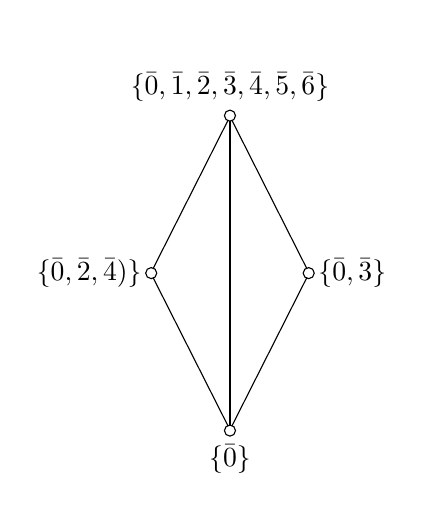
\begin{tikzpicture}
	\draw (0,0)node[left]{$\{\bar{0},\bar{2},\bar{4})\}$}
	(0.025,0.06)--(0.975,1.94);
	\draw (0.025,-0.06)--(0.975,-1.94);
	\draw (1.025,1.94)--(1.975,0.06);
	\draw (1.025,-1.94)--(1.975,-0.06) (2,0)node[right]{$\{\bar{0},\bar{3}\}$};
	\draw (1,-1.93) node[below=3.5pt]{$\{\bar{0}\}$}--(1,1.93) node[above=3.5pt]{$\{\bar{0},\bar{1},\bar{2},\bar{3},\bar{4},\bar{5},\bar{6}\}$} ;
	\draw (0,0) circle [radius=2pt] ;
	\draw (1,2) circle [radius=2pt];
	\draw (1,-2) circle [radius=2pt];
	\draw (2,0) circle [radius=2pt];
	\draw (0,3) node[]{};
	\end{tikzpicture}	
\end{center}

\end{solution}	


\subsection{\textsection7. Quotient groups}
\begin{problem}[7.1]
$\vartriangleright$ List all subgroups of $S_3$ (cf. \hyperlink{Exercise II.6.13}{Exercise II.6.13}) and determine which subgroups are normal and which are not normal. [\textsection7.1]
\end{problem}
\begin{solution}
	The subgroups of $S_3$ are $\{(1)\},\{(1),(12)\},\{(1),(13)\},\{(1),(23)\},\{(1),(123),(132)\}$ and $S_3$. We can check that $\{(1)\},\{(1),(123),(132)\},S_3$ are normal subgroups while others are not.
\end{solution}	

\begin{problem}[7.2]
Is the image of a group homomorphism necessarily a normal subgroup of the target?
\end{problem}
\begin{solution}
No. According to exercise 7.1 we have seen not all subgroups are normal. Suppose $H$ is a subgroup of $G$ but not normal. Then $H$ itself is the image of the inclusion homomorphism $i:H\hookrightarrow G$, which makes a counterexample.   
\end{solution}

\begin{problem}[7.3]
$\vartriangleright$ Verify that the equivalent conditions for normality given in §7.1 are indeed equivalent. [\textsection7.1]
\end{problem}
\begin{solution}
That a subgroup $N$ of $G$ is normal has four equivalent conditions:
\begin{enumerate}
	\item[(i)] $\forall g\in G,\ gNg^{-1}= N$;
	\item[(ii)] $\forall g\in G,\ gNg^{-1}\subseteq N$;
	\item[(iii)] $\forall g\in G,\ gN\subseteq Ng$;
	\item[(iv)] $\forall g\in G,\ gN= Ng$.
\end{enumerate}
(i)$\implies$(ii) is straightforward. \\
(ii)$\implies$(iii). For any $g\in G$, the element $a\in gN$ can be written as $a=gn_1(n_1\in N)$. Since $gn_1g^{-1}\in gNg^{-1}\subseteq N$, there exists an $n_2\in N$ such that $gn_1g^{-1}=n_2$, which implies $gn_1=n_2g\in Ng$. Thus we have $gN\subseteq Ng$.\\	
(iii)$\implies$(iv). Given any $g\in G$, for all $n_1\in N$, the element $g^{-1}n_1\in g^{-1}N_1$ also belongs to $Ng^{-1}$, which implies that there exists $n_2\in N$ such that $g^{-1}n_1=n_2g^{-1}$, namely $n_1g=gn_2$. Thus we get $Ng\subseteq gN$ and accordingly $gN= Ng$.\\
(iv)$\implies$(i). For any $g\in G$, the element $b\in gNg^{-1}$ can be written as $a=gn_1g^{-1}(n_1\in N)$. Since $gn_1\in gN= Ng$, there exists an $n_2\in N$ such that $gn_1=n_2g$, which implies $gn_1g^{-1}=n_2\in N$. Thus we have 
\begin{align*}
	&\forall g\in G,\quad gNg^{-1}\subseteq N\\
	\implies& \forall g^{-1}\in G,\quad g^{-1}(gNg^{-1})g\subseteq gNg^{-1}\\
	\implies& \forall g\in G,\quad N\subseteq gNg^{-1}.
\end{align*}
Hence we have $\forall g\in G,\ gNg^{-1}=N$.
\end{solution}


\begin{problem}[7.4]
Prove that the relation defined in \hyperlink{Exercise II.5.10}{Exercise II.5.10} on a free abelian group $F =F^{ab}(A)$ is compatible with the group structure. Determine the quotient $F/\sim$ as a better known group.
\end{problem}
\begin{solution}
For all $f,f',h\in F$,
\[
f\sim f'\iff f-f'=2g,\,(g\in F)\implies (h+f)-(h+f')=2g,\,(g\in F)\iff h+f\sim h+f'.
\]
Since $F$ is abelian, wee see the relation $\sim$ defined on a free abelian group $F =F^{ab}(A)$ is compatible with the group structure. By the notation of quotient group, we have 
\[
F/\hspace{-2pt}\sim\hspace{4pt}=F/2F,
\]
where $2F=\{2g\in F\,|\,g\in F\}$.
\end{solution}


\begin{problem}[7.5]
$\neg$ Define an equivalence relation $\sim$ on $\SL_2(\Z)$ by letting $A\sim A'\iff A'=\pm A.$ Prove that $\sim$ is compatible with the group structure. The quotient $\SL_2(\Z)/\sim$ is denoted $\mathrm{PSL}_2(\Z)$, and is called the \emph{modular group}; it would be a serious contender in a context for \textquoteleft the most important group in mathematics', due to its role in algebraic geometry and number theory. Prove that $\mathrm{PSL}_2(\Z)$ is generated by the (cosets of the) matrices
\[
\begin{pmatrix}
0 & -1\\
1 & 0\\
\end{pmatrix}
\quad\text{ and }\quad 
\begin{pmatrix}
1 & -1\\
1 & 0\\
\end{pmatrix}.
\]
(You will not need to work very hard, if you use the result of \hyperlink{Exercise 6.10}{Exercise 6.10}.) Note that the first has order 2 in $\mathrm{PSL}_2(\Z)$, the second has order 3, and their product has infinite order. [9.14]
\end{problem}
\begin{solution}
For all $A_1,A_2,B\in \SL_2(\Z)$,
\[
A_1\sim A_2\iff A_2=\pm A_1\iff  BA_2=\pm BA_1\iff BA_1\sim BA_2.
\]	
Hence $\sim$ is compatible with the group structure and $\mathrm{PSL}_2(\Z)=\SL_2(\Z)/\{I_2,-I_2\}$. In \hyperlink{Exercise 6.10}{Exercise 6.10} we have shown $\SL_2(\Z)$ is generated by the matrices
\[
s =
\begin{pmatrix}
0 & -1\\
1 & 0\\
\end{pmatrix}
\quad\text{ and }\quad 
t =
\begin{pmatrix}
1 & 1\\
0 & 1\\
\end{pmatrix}.
\] 
It is clear that $\SL_2(\Z)$ can also be generated by the matrices
\[
s =
\begin{pmatrix}
0 & -1\\
1 & 0\\
\end{pmatrix}
\quad\text{ and }\quad 
ts =
\begin{pmatrix}
1 & -1\\
1 & 0\\
\end{pmatrix},
\] 
which implies $\mathrm{PSL}_2(\Z)$ is generated by the cosets of the matrices $s$ and $ts$.
\end{solution}

\begin{problem}[7.6]
Let $G$ be a group, and let $n$ be a positive integer. Consider the relation
\[
a\sim b\iff(\exists g\in G)ab^{-1}=g^n.
\]
\begin{itemize}
	\item Show that in general $\sim$ is not an equivalence relation.
	\item Prove that $\sim$ is an equivalence relation if $G$ is commutative, and determine the corresponding subgroup of $G$.
\end{itemize}

\end{problem}
\begin{solution}
\begin{itemize}
	\item Let $G$ be the symmetric group $S_4$ and let $n=2$. We can check that
	\begin{align*}
		&(3\ 4)(2\ 3)^{-1}=(2\ 4\ 3)=(2\ 3\ 4)^2\implies(3\ 4)\sim (2\ 3)\\
		&(2\ 3)(1\ 2)^{-1}=(1\ 3\ 2)=(1\ 2\ 3)^2\implies(2\ 3)\sim (1\ 2)
	\end{align*}
	but $(3\ 4)(1\ 2)^{-1}=(1\ 2)(3\ 4)$ is not the square of any element in $S_4$.
	\item Suppose that $G$ is commutative. $aa^{-1}=e^n$ implies $\sim$ is reflexive. Since
	\[
	a\sim b\implies ab^{-1}=g^n\;(g\in G)\implies b^{-1}a=g^{-n}\;(g^{-1}\in G)\implies b\sim a,
	\]  
	$\sim$ is symmetric. Since $G$ is commutative, we have
	\begin{align*}
		&a\sim b,b\sim c\implies ab^{-1}=g_1^n,bc^{-1}=g_2^n\;(g_1,g_2\in G)\\
		\implies& ac^{-1}=ab^{-1}bc^{-1}=g_1^ng_2^n=(g_1g_2)^n\;(g_1g_2\in G)\implies a\sim c,
	\end{align*}
	which means $\sim$ is transitive. Thus we show that $\sim$ is an equivalence relation. Since
	\[
	a\sim b\implies ab^{-1}=g^n\implies ga(gb)^{-1}=(ag)(bg)^{-1}=g^n\implies ga\sim gb,ag\sim bg,
	\]
	we see $\sim$ is compatible with the group $G$ and the equivalence class of the identity $H=\{g^n|g\in G\}$ is a subgroup of $G$.
\end{itemize}
\end{solution}

\begin{problem}[7.7]
	Let $G$ be a group, $n$ a positive integer, and let $H \subseteq G$ be the subgroup
	generated by all elements of order $n$ in $G$. Prove that $H$ is normal.
\end{problem}
\begin{solution}
	For all $h\in H, g\in G$, we have 
	$$(ghg^{-1})^n=gh^ng^{-1}=gg^{-1}=e_G\implies ghg^{-1}\in H,  $$
	which means $gHg^{-1}\subseteq H$ for all $g\in G$. Thus we show that $H$ is normal.
\end{solution}

\begin{problem}[7.10]
$\neg$ Let $G$ be a group, and $H\subseteq G$ a subgroup. With notation as in \hyperlink{Exercise II.6.7}{Exercise II.6.7}, show that $H$ is normal in $G$ if and only if $\forall \gamma \in \Inn(G), \gamma(H) \subseteq H$.
Conclude that if $H$ is normal in $G$ then there is an interesting homomorphism
$\Inn(G)\to \Aut(H)$. [8.25]
\end{problem}
\begin{solution}
Consistent with the notation as in \hyperlink{Exercise II.6.7}{Exercise II.6.7}, suppose
\[
\gamma_g:G\longrightarrow G,\ h\longmapsto ghg^{-1}.
\]
Then we have
\[
\forall \gamma_g \in \Inn(G), \gamma_g(H) \subseteq H\iff \forall g\in G, gHg^{-1}\subseteq H\iff \text{$H$ is normal in $G$}.
\]
Thus we see that if $H$ is normal in $G$, $\gamma$ can be restricted to $H$ so that $\gamma|_H:H\rightarrow H$ is an automorphism on $H$. Let 
\[
i:\Inn(G)\longrightarrow \Aut(H),\ \gamma\longmapsto\gamma|_h
\]
and with the property of $\gamma$ we have shown in \hyperlink{Exercise II.4.8}{Exercise II.4.8}, it is straightforward to check that
\[
i(\gamma_{g_1}\gamma_{g_2})=i(\gamma_{g_1g_2})=\gamma_{g_1g_2}|_h=(\gamma_{g_1}\gamma_{g_2})|_h=\gamma_{g_1}|_h\gamma_{g_2}|_h=i(\gamma_{g_1})i(\gamma_{g_2}).
\]
That is, $i$ is the interest homomorphism $\Inn(G)\to \Aut(H)$ that we expect.
\end{solution}

\hypertarget{Exercise II.7.11}{}
\begin{problem}[7.11]
$\vartriangleright$ Let $G$ be a group, and let $[G,G]$ be the subgroup of $G$ generated by all elements of the form $aba^{-1}b^{-1}$. (This is the commutator subgroup of $G$; we will return to it in \textsection IV.3.3.) Prove that $[G,G]$ is normal in $G$. (Hint: with notations in \hyperlink{Exercise II.4.8}{Exercise II.4.8}, $gaba^{-1}b^{-1}g^{-1} = \gamma_g(aba^{-1}b^{-1})$.) Prove that $[G,G]$ is normal in $G$. [7.12, \textsection IV.3.3]
\end{problem}
\begin{solution}
Since for all $g\in G, aba^{-1}b^{-1}\in[G,G]$, we have
\[
gaba^{-1}b^{-1}g^{-1}=gag^{-1}gbg^{-1}ga^{-1}g^{-1}gb^{-1}g^{-1}=(gag^{-1})(gbg^{-1})(gag^{-1})^{-1}(gbg^{-1})^{-1}\in[G,G],
\]
it follows that that $[G,G]$ is normal in $G$. Then we can show $[G,G]$ is normal in $G$ by
\[
[g_1][g_2]=[g_1g_2]=[g_1g_2(g_2^{-1}g_1^{-1}g_2g_1)]=[g_2g_1]=[g_2][g_1],\quad\forall [g_1],[g_2]\in[G,G].
\]
\end{solution}

\hypertarget{Exercise II.7.12}{}
\begin{problem}[7.12]
$\vartriangleright$ Let $F = F(A)$ be a free group, and let $f : A\to G$ be a set-function
from the set $A$ to a commutative group $G$. Prove that $f$ induces a unique homomorphism $F/[F, F]\to G$, where $[F, F]$ is the commutator subgroup of $F$ defined in \hyperlink{Exercise II.7.11}{Exercise II.7.11}. (Use Theorem 7.12.) Conclude that $F/[F, F]\simeq F^{ab}(A)$. (Use Proposition I.5.4.) [\textsection6.4, 7.13, VI.1.20]
\end{problem}
\begin{solution}
By the universal property of free group, there exists a unique homomorphism $\varphi:F\to G$ such that $\forall a\in A,\;\varphi(j(a))=f(a)$ 
where $j:A\to F(A)$ is a inclusion. Note that $G$ is commutative, we have
\[
\varphi(aba^{-1}b^{-1})=\varphi(a)\varphi(b)\varphi(a)^{-1}\varphi(b)^{-1}=e_G,
\]
which implies $[F,F]\subseteq \ker\varphi$. Theorem 7.12 indicates that there exists a unique group homomorphism $\tilde{\varphi}:F/[F, F]\to G$ so that $\tilde{\varphi}\circ\pi=\varphi$. Now we deduce that the diagram
\[\xymatrix{
	A\ar@{->}[d]_{j}\ar@{->}[rd]^{f} \\
	F\ar@{->}[r]^{\exists!\varphi}\ar@{->}[d]_{\pi} & G\\
	F/[F,F]\ar@{->}[ru]_{\exists!\tilde{\varphi}}  
}\]
commutes. For the diagram we see $\tilde{\varphi}\circ\pi\circ j=f$. Suppose there exists $\psi$ such that $\psi\circ\pi\circ j=f$, which amounts to $(\psi\circ\pi)\circ j=\varphi\circ j$. By the uniqueness of $\varphi$ we have $\psi\circ\pi=\varphi$. Then by the uniqueness of $\tilde{\varphi}$ we have $\psi=\tilde{\varphi}$. Thus we show that there exists unique $\tilde{\varphi}$ such that $\tilde{\varphi}\circ\pi\circ j=f$. According to the property of free abelian group, we can conclude that $F/[F, F]\simeq F^{ab}(A)$.
\end{solution}

\begin{problem}[7.13]
$\neg$ Let $A, B$ be sets, and $F(A), F(B)$ the corresponding free groups. Assume $F(A)\simeq F(B)$. If $A$ is finite, prove that so is $B$, and $A\simeq B$. (Use \hyperlink{Exercise II.7.12}{Exercise II.7.12} to upgrade \hyperlink{Exercise II.5.10}{Exercise II.5.10}.) [5.10, VI.1.20]
\end{problem}
\begin{solution}
\hyperlink{Exercise II.7.12}{Exercise II.7.12} tells us that the free abelian group generated by a set is merely determined by its free group, which means
\[
F(A)\simeq F(B)\implies F(A)/[F(A),F(A)]\simeq F(B)/[F(B),F(B)]\implies F^{ab}(B)\cong F^{ab}(A).
\]
Then under the auspices of the conclusion in \hyperlink{Exercise II.5.10}{Exercise II.5.10} we complete the proof.
\end{solution}


\subsection{\textsection8. Canonical decomposition and Lagrange's theorem}
\begin{problem}[8.1]
	If a group $H$ may be realized as a subgroup of two groups $G_1$ and $G_2$, and
\[
	\frac{G_1}{H}\cong \frac{G_2}{H},
\]
does it follows that $G_1\cong G_2$. Give a proof or a counterexample.
\end{problem}
\begin{solution}
	A counterexample is given as follows. Take $H=C_3$, the cyclic group of order $3$. Take $G_1=D_6$ and $G_2=C_6$, then one sees both $G_1/H$ and  $G_2/H$ are $C_2$. But obviously $G_1$ and $G_2$ are not isomorphic, one being abelian while the other is not.
\end{solution}

\begin{problem}[8.2]
$\neg$ Extend Example 8.6 as follows. Suppose $G$ is a group, and $H\subseteq G$ is a subgroup of index 2: that is, such that there are precisely two (say, left) cosets of $H$ in $G$. Prove that $H$ is normal in $G$. [9.11, IV.1.16]
\end{problem}
\begin{solution}
Since $[G/H]=2$, there must be $G/H=\{H,G-H\}$. For any $g\in G	$: 
\begin{itemize}
	\item if $g\in H$, then $gH=Hg=H$;
	\item if $g\in G-H$, then $gH\ne H$ and $Hg\ne H$. Thus we have $gH=Hg=G-H$.
\end{itemize}
In either case $gH=Hg$ holds for all $g\in G$, which implies $H$ is normal in $G$.
\end{solution}

\begin{problem}[8.7]
Let $(A|\mathscr{R})$, resp. $(A'|\mathscr{R}')$ be presentations for two groups $G$, resp. $G'$(cf. §8.2); we may assume that $A, A'$ are disjoint. Prove that the group $G*G'$ presented by
\[
(A\cup A'|\mathscr{R}\cup \mathscr{R}')
\]
satisfies the universal property for the \emph{coproduct} of $G$ and $G'$ in $\Grp$. (Use the universal properties of both free groups and quotients to construct natural homomorphisms $G\to G*G'$, $G'\to G* G'$.) [\textsection3.4, \textsection8.2, 9.14].
\end{problem}
\begin{solution}
Assume that $F(A)/R=(A|\mathscr{R})$, $F(A')/R'=(A|\mathscr{R}')$, and $F(A\amalg A')/R''=(A\cup A'|\mathscr{R}\cup \mathscr{R}')$.
	\[\xymatrix{
		&G&\\
		F(A)/R\ar[ru]^{f}\ar@{-->}[r]^{\psi\hspace{1em}}&F(A\amalg A')/R''\ar@{-->}[u]^{\delta}&F(A')/R'\ar[lu]_{f'}\ar@{-->}[l]_{\hspace{1em}\psi'}\\
		A\ar[rd]_{i}\ar[u]^{k}&F(A\amalg A')\ar[u]_{\pi}&A'\ar[ld]^{i'}\ar[u]_{k'}\\
		&A\amalg A'\ar[u]_{j} &
	}\]
According to \hyperlink{Lemma II.1}{Lemma II.1}, there exist unique $\psi$ and $\psi'$ such that 
\[
\psi\circ k=\pi\circ j\circ i,\ \psi'\circ k'=\pi\circ j\circ i'.
\]
Define 
\begin{align*}
\delta:&F(A\amalg A')/R''\longrightarrow G\\
&[\{a_1\}*\{a_1'\}*\cdots*\{a_n\}*\{a_n'\}]\longmapsto f([\{a_1\}])f'([\{a_1'\}])\cdots f([\{a_n\}])f'([\{a_n'\}]).
\end{align*}
where $*$ means the junction of words and $\{a_i\}=a_{i1}*a_{i2}*\cdots *a_{im_i}$, $a_{ij}\in A$ $(1\le i\le n,1\le j\le m_i)$ and $\{a_i'\}=a_{i1}'*a_{i2}'*\cdots *a_{im_i'}$, $a_{ij'}\in A$ $(1\le i\le n,1\le j'\le m_i')$.
It is routine to check that $\delta$ is a well-defined homomorphism such that 
$$
\delta\circ\psi=f,\ \delta\circ\psi'=f'.
$$ 
Then verify that if $\hat{\delta}$ is a homomorphism such that 
$$
\delta\circ\psi=f,\ \delta\circ\psi'=f',
$$ 
there must be $\hat{\delta}=\delta$. After these tasks are done, we can conclude that $F(A\amalg A')/R''$ satisfies the universal property of coproduct.

\end{solution}


\begin{problem}[8.17]
$\triangleright$ Assume $G$ is a finite abelian group, and let $p$ be a prime divisor of $|G| .$ Prove that there exists an element in $G$ of order $p$. (Hint: let $g$ be any element of $G,$ and consider the subgroup $\langle g\rangle$; use the fact that this subgroup is cyclic to show that there is an element $h \in\langle g\rangle$ in $G$ of prime order $q .$ If $q=p$ you are done; else, use the quotient $G /\langle h\rangle$ and induction.) $[\S 8.5,8.18,8.20, \S \mathrm{IV} .2 .1]$
\end{problem}
\begin{solution}
Suppose the proposition to be poven holds for $k=|G|\le N-1$. Now assume that $k=|G|=N$. Let $g$ be any element of $G$ such that $g\ne e_G$ and consider the cyclic group $\langle g\rangle$. We are to show that there is an element $h \in\langle g\rangle$ of prime order $q$. If $|\langle g\rangle|$ is prime, simply take $h=g$. If $|\langle g\rangle|$ is not prime, we can assume that $|\langle g\rangle|=rs$, where $r,s\in\mathbb{Z}$ and $r$ is prime. Note
\[
\left|g^{s}\right|=\frac{|g|}{\operatorname{gcd}(s,|g|)}=\frac{rs}{\operatorname{gcd}(s,rs)}=\frac{rs}{s}=r.
\]
We can take $h=g^{s}$. Therefore, there is an element $h \in\langle g\rangle$ such that $q=|h|$ is prime. If $q=p$, the proof is completed. Otherwise, let $G_1=G /\langle h\rangle$. It still follows that $G_1$ is a finite abelian group and $p$ is a prime divisor of $|G_1|$. Since $k=|G_1|=N/q\le N-1$, by induction it follows that there exists an element $x\langle h\rangle\in G_1$ of order $p$. Thus we have
\[
x^p\langle h\rangle=\langle h\rangle\implies x^p=h^m\implies x^{pq}=h^{mq} \implies (x^{q})^p=e_G\implies |x^{q}|\mid p\implies|x^{q}|=1\text{ or }p.
\]
If $x^{q}=e_G$, then 
$$
x^{q}\langle h\rangle=\langle h\rangle\implies|x\langle h\rangle|\mid q\implies p\mid q,
$$
which leads to a contradiction. Thus there must be $|x^{q}|=p$, which means the proposition holds when $k=|G|=N$. By induction we prove that there exists an element in $G$ of order $p$.

\end{solution}

\begin{problem}[8.18]
Let $G$ be an abelian group of order $2 n$, where $n$ is odd. Prove that $G$ has exactly one element of order $2 .$ (It has at least one, for example by Exercise 8.17. Use Lagrange's theorem to establish that it cannot have more than one.) Does the same conclusion hold if $G$ is not necessarily commutative?
\end{problem}
\begin{solution}
By Exercise 8.17, $G$ has exactly one element of order $2$. Suppose $a,b$ are two distinct elements of order $2$. Consider the generated subgroup 
$$
\langle a,b\rangle=\{e,a,b,ab\}.
$$
According to Lagrange's theorem, since $|\langle a,b\rangle|=4$, there must be $4|2n$ or $2|n$, where $n$ is odd. That is a contradiction. Thus we see $G$ cannot have two distinct elements of order $2$, which implies that $G$ has exactly one element of order $2$.

\end{solution}




\subsection{\textsection9. Group actions}

\subsection{\textsection10. Group objects in categories}

\newpage
\section{Chapter III\hspace{0.2em} Rings and modules}

\subsection{\textsection1. Definition of ring}
\begin{problem}[1.1]
	$\vartriangleright$ Prove that if $0 = 1$ in a ring $R$, then $R$ is a zero-ring. [\textsection1.2]
\end{problem}
\begin{solution}
	For any $x$ in the ring $R$, we have
	\[
	1\cdot x=x,\qquad 0\cdot x=0.
	\]
	Since $0 = 1$ we see that $x=0$, which implies $R$ is a ring with only one element $0$.
\end{solution}


\hypertarget{Exercise III.1.2}{}
\begin{problem}[1.2]
	$\neg$ Let $S$ be a set, and define operations on the power set $\mathscr{P}(S)$ of $S$ by setting $\forall A,B \in \mathscr{P}(S)$
	\[
	A+B :=(A \cup B) \backslash(A \cap B) \quad, \quad A \cdot B=A \cap B
	\]
	Prove that $(\mathscr{P}(S),+,\cdot)$ is a commutative ring. [2.3, 3.15]
\end{problem}
\begin{solution}
	First, we need to check that $(\mathscr{P}(S),+)$ is an abelian group:
	\begin{itemize}
		\item associativity:	
		\begin{align*}
		&\hspace{1em}(A+B)+C\\
		&=((A \cup B) \backslash(A \cap B))+C\\
	    &=((A \cup B) \cap(A^C \cup B^C))+C\\
	    &=(A\cap(A^C \cup B^C) )\cup (B\cap(A^C \cup B^C)) +C\\
	    &=(A \cap B^C) \cup(A^C \cap B)+C\\
	    &=(((A \cap B^C) \cup(A^C \cap B)) \cap C^C) \cup(((A \cap B^C) \cup(A^C \cap B))^C \cap C)\\
	    &=((A \cap B^C\cap C^C )\cup(A^C \cap B\cap C^C) ) \cup((A^C \cup B) \cap(A\cup B^C)\cap C)\\
	    &=((A \cap B^C\cap C^C )\cup(A^C \cap B\cap C^C) ) \cup((A^C\cap B^C) \cup( A\cap B) \cap C)\\
	    &=(A \cap B^C\cap C^C )\cup(A^C \cap B\cap C^C)  \cup(A^C\cap B^C\cap C) \cup( A\cap B\cap C) \\
	    &=(A \cap (B \cap C) \cup(B^C \cap C^C)) \cup((A^C \cap B \cap C^C) \cup (A^C \cap B^C \cap C))\\
	    &=(A \cap (B^C \cup C) \cap(B \cup C^C)) \cup((A^C \cap B \cap C^C) \cup (A^C \cap B^C \cap C))\\
	    &=(A \cap ((B \cap C^C) \cup(B^C \cap C))^C) \cup(A^C \cap ((B \cap C^C) \cup(B^C \cap C)))\\
	    &=A+((B \cap C^C) \cup(B^C \cap C))\\
	    &=A+(B+C);
		\end{align*}
		\item commutativity:
		\[
		A+B =(A \cup B) \backslash(A \cap B)=(B \cup A) \backslash(B \cap A)= B+A;
		\]
		\item additive identity: the additive identity is $\varnothing$ since
		\[
		A+\varnothing=(A \cup \varnothing) \backslash(A \cap \varnothing)=A; \backslash\varnothing=A
		\] 
		\item inverse: the inverse of some set $A$ is just itself since
		\[
		A+A=(A \cup A) \backslash(A \cap A)=A\backslash A=\varnothing.
		\]
	\end{itemize}
	Then we have to show that $(\mathscr{P}(S),\cdot)$ is a commutative monoid, which clearly holds with the multiplicative identity $S$. What is left to show is the distributive properties and the check is straightforward.
	\begin{align*}
	&\hspace{1em}(A+B)\cdot C\\
	&=((A \cap B^C) \cup(A^C \cap B))\cap C\\
	&=(A \cap B^C\cap C) \cup(A^C \cap B\cap C)\\
	&=(A\cap C \cap (B^C\cup C^C)) \cup((A^C\cup C^C) \cap (B\cap C))\\
	&=(A\cap C \cap (B\cap C)^C) \cup((A\cap C)^C \cap (B\cap C))\\
	&=A\cdot C+B\cdot C.
	\end{align*}
\end{solution}

\begin{problem}[1.3]
	$\neg$ Let $R$ be a ring, and let $S$ be any set. Explain how to endow the set $R^S$ of set-functions $S\to R$ of two operations $+$, $\cdot$ so as to make $R^S$ into a ring, such that $R^S$ is just a copy of $R$ if $S$ is a singleton. [2.3]
\end{problem}
\begin{solution}
	To make $(R^S,+,\cdot )$ a ring , for all $f,g\in R^S$ we define addition and multiplication as
	\begin{align*}
	f+g&:S\longrightarrow R,\quad x\longmapsto f(x)+g(x)\\
	f\cdot g&:S\longrightarrow R,\quad x\longmapsto f(x)\cdot g(x).
	\end{align*}
\end{solution}

\hypertarget{Exercise III.1.4}{}
\begin{problem}[1.4]
	$\vartriangleright$ The set of $n\times n$ matrices with entries in a ring $R$ isdenoted $\mathcal{M}_n(R)$. Prove that componentwise addition and matrix multiplication makes $\mathcal{M}_n(R)$ into a ring, for any ring $R$. The notation $\mathfrak{gl}_n(R)$ is also commonly used, especially $R=\mathbb{R}$ or $\mathbb{C}$ (although this indicates one is considering them as \emph{Lie algebras}) in parallel with the analogous notation for the corresponding groups of units, cf. \hyperlink{Exercise II.6.1}{Exercise II.6.1}. In
	fact, the parallel continues with the definition of the following sets of matrices:
	\begin{itemize}
		\item $\mathfrak{sl}_n(\mathbb{R}) = \{M \in \mathfrak{gl}_n(\mathbb{R}) | \mathrm{tr}(M) = 0\}$;
		\item $\mathfrak{sl}_n(\mathbb{C}) = \{M \in \mathfrak{gl}_n(\mathbb{C}) | \mathrm{tr}(M) = 0\}$;
		\item $\mathfrak{so}_n(\mathbb{R}) = \{M \in \mathfrak{sl}_n(\mathbb{R}) |M +M^t = 0\}$;
		\item $\mathfrak{su}(n) = \{M \in \mathfrak{sl}_n(\mathbb{C}) |M +M^\dag = 0\}$.
	\end{itemize}
	Here $\mathrm{tr}(M)$ is the trace of $M$, that is, the sum of its diagonal entries. The other notation matches the notation used in Exercise II.6.1. Can we make rings of these sets, by endowing them of ordinary addition and multiplication of matrices? (These sets are all Lie algebras, cf. Exercise VI.1.4.) [\textsection1.2, 2.4, 5.9, VI.1.2, VI.1.4]
\end{problem}
\begin{solution}
	It is plain to show $\mathcal{M}_n(R)$ is a ring according to the definition. For multiplicative associativity, it follows that for all $A,B,C\in\mathcal{M}_n(R)$,
	\begin{align*}
	&\hspace{1em}((A B) C)_{\alpha, \delta}\\
	&=\sum_{i=1}^{n}(A B)_{\alpha, i} c_{i, \delta}\\
	&=\sum_{i=1}^{n}\left(\sum_{j=1}^{n} a_{\alpha, j} b_{j, i}\right) c_{i, \delta}\\
	&=\sum_{i=1}^{n} \sum_{j=1}^{n}\left(a_{\alpha, j} b_{j, i}\right) c_{i, \delta}\\
	&=\sum_{j=1}^{n} \sum_{n=1}^{n} a_{\alpha, j}\left(b_{j, i} c_{i, \delta}\right)\\
	&=\sum_{j=1}^{n} a_{\alpha, j}\left(\sum_{i=1}^{n} b_{j, i} c_{i, \delta}\right)\\
	&=\sum_{j=1}^{n} a_{\alpha, j}(B C)_{j, \delta}\\
	&=(A(B C))_{\alpha, \delta}.
	\end{align*}
	Under the ordinary addition and multiplication of matrices, $\mathfrak{sl}_n(\mathbb{R}),\mathfrak{sl}_n(\mathbb{C}),\mathfrak{so}_n(\mathbb{R}),\mathfrak{su}_n(\mathbb{C})$ are not rings. In fact, they are not closed under the multiplication.
\end{solution} 

\begin{problem}[1.5]
	Let $R$ be a ring. If $a, b$ are zero-divisors in $R$, is $a+b$ necessarily a zero-divisor?
\end{problem}
\begin{solution}
	That is not true. Let's take $\mathbb{Z}/6\mathbb{Z}$ as an counterexample. Though both $[2]_6$ and $[3]_6$ are zero-divisors, their sum $[5]_6$ is not a zero-divisor.
\end{solution}

\hypertarget{Exercise III.1.6}{}
\begin{problem}[1.6]
	$\neg$ An element $a$ of a ring $R$ is \emph{nilpotent} if $a^n = 0$ for some $n$.
	\begin{enumerate}
	\item Prove that if $a$ and $b$ are nilpotent in $R$ and $ab = ba$, then $a+b$ is also nilpotent.
	\item Is the hypothesis $ab = ba$ in the previous statement necessary for its conclusion to hold?
	\end{enumerate}
[3.12]
\end{problem}
\begin{solution}
	\begin{enumerate}
		\item Assume that $a^n=b^m=0$ and let $k=2\max\{n,m\}$. If $ab = ba$, we can get
		\[
		(a+b)^k=\sum_{p=0}^{\tfrac{k}{2}}\binom{k}{p}a^kb^{k-p}+\sum_{p=\tfrac{k}{2}+1}^{k}\binom{k}{p}a^kb^{k-p}=\sum_{p=0}^{\tfrac{k}{2}}\binom{k}{p}a^k\cdot 0+\sum_{p=\tfrac{k}{2}+1}^{k}\binom{k}{p}0\cdot b^{k-p}=0,
		\]
		which means $a+b$ is also nilpotent.
		\item The hypothesis $ab = ba$ is necessary. A counterexample can be found in the ring $\mathfrak{gl}_2(\mathbb{R})$. Let
		\[
		a=\left(
		\begin{matrix}	
		0 & 1\\	
		0 & 0	
		\end{matrix}
		\right),\quad
		b=\left(
		\begin{matrix}	
		0 & 0\\	
		1 & 0	
		\end{matrix}
		\right)
		\]
		and then we have $a^2=b^2=0$. In other words, $a$ and $b$ are nilpotent. However, by diagonalization we see that
		\[
		(a+b)^n=
		\left(
		\begin{matrix}	
		0 & 1\\	
		1 & 0	
		\end{matrix}
		\right)^n
		=\left(
		\begin{matrix}	
		-1 & 1\\	
		1 & 1	
		\end{matrix}
		\right)
		\left(
		\begin{matrix}	
		-1 & 0\\	
		0 & 1	
		\end{matrix}
		\right)^n
		\left(
		\begin{matrix}	
		-1 & 1\\	
		1 & 1	
		\end{matrix}
		\right)^{-1}\ne 
		\left(
		\begin{matrix}	
		0 & 0\\	
		0 & 0	
		\end{matrix}
		\right).
		\]
		Thus in such case, $a+b$ is no longer nilpotent.
	\end{enumerate}
\end{solution}

\begin{problem}[1.8]
	Prove that $x = \pm1$ are the only solutions to the equation $x^2 = 1$ in an integral	domain. Find a ring in which the equation $x^2 = 1$ has more than 2 solutions.
\end{problem}
\begin{solution}
	It clearly holds that $1\cdot1=1$ and $(-1)\cdot(-1)=((-1)\times(-1))1\cdot1=1$. That is to say,  $x = \pm1$ are the solutions to the equation $x^2 = 1$. Note that if there exists $x$ in an integral	domain such that $x^2=1$, then we have
	\[
	(x-1)\cdot(x+1)=x^2-1=0,
	\]
	which implies $x-1=0$ or $x+1=0$. Therefore, we can assert $x = \pm1$ are the solutions. In the ring $\mathbb{Z}/8\mathbb{Z}$, $[3]_8$ and $[5]_8$ are also the solutions to the equation $x^2 = 1$.
\end{solution}

\begin{problem}[1.10]
	Let $R$ be a ring. Prove that if $a \in R$ is a right unit, and has two or more left-inverses, then $a$ is not a left-zero-divisor, and is a right-zero-divisor.
\end{problem}
\begin{solution}
	Since $a \in R$ is a right unit, it cannot be a left-zero-divisor. Assume there exist two distinct elements $x,y\in R$ such that $xa=ya=1$ and it deduces $(y-x)a=0$. Thus we show that $a$ a right-zero-divisor.
\end{solution}

\begin{problem}[1.11]
	Construct a field with 4 elements: as mentioned in the text, the underlying
	abelian group will have to be $\mathbb{Z}/2\mathbb{Z}\times\mathbb{Z}/2\mathbb{Z}$; $(0, 0)$ will be the zero element, and (1, 1) will be the multiplicative identity. The question is what $(0, 1)\cdot(0, 1)$, $(0, 1)\cdot(1, 0)$, $(1, 0)\cdot(1, 0)$ must be, in order to get a field. [\textsection1.2, \textsection V.5.1]
\end{problem}
\begin{solution}
	Define 
	\[
	(0, 1)\cdot(0, 1)=(0, 1),\quad (0, 1)\cdot(1, 0)=(0,0),\quad (1, 0)\cdot(1, 0)=(1, 0),
	\]
	and the the rest definition of multiplication will be determined uniquely according to field properties. For example, we have no alternatives but to define
	\[
	(0, 1)\cdot(1,1)=(0, 1)\cdot((0,1)+(1,0))=(0, 1)\cdot(0,1)+(0, 1)\cdot(1,0)=(0, 1)+(0,0)=(0,1).
	\]
	Then we can check $\mathbb{Z}/2\mathbb{Z}\times\mathbb{Z}/2\mathbb{Z}$ forms a field by definition. 
\end{solution}

\hypertarget{Exercise III.1.4}{}
\begin{problem}[1.12]
	Just as complex numbers may be viewed as combinations $a+bi$, where
	$a,b\in \R$, and $i$ satisfies the relation $i^2=-1$ (and commutes with $\R$), we may construct a ring $\mathbb{H}$ by considering linear combinations $a + bi + cj + dk$ where $a, b, c, d \in \R$, and $i, j, k$ commute with $\R$ and satisfy the following relations:
	\[
	i^{2}=j^{2}=k^{2}=-1 \quad, \quad i j=-j i=k \quad, \quad j k=-k j=i \quad, \quad k i=-i k=j.
	\]
	Addition in $\mathbb{H}$ is defined componentwise, while multiplication is defined by imposing	distributivity and applying the relations. For example,
	\[
	(1+i+j) \cdot(2+k)=1 \cdot 2+i \cdot 2+j \cdot 2+1 \cdot k+i \cdot k+j \cdot k=2+2 i+2 j+k-j+i=2+3 i+j+k.
	\]
	\begin{enumerate}[(i)]
		\item Verify that this prescription does indeed define a ring.
		\item Compute $(a+b i+c j+d k)(a-b i-c j-d k)$, where $a, b, c, d \in \R$.
		\item Prove that $\mathbb{H}$ is a division ring. Elements of $\mathbb{H}$ are called quaternions. Note that $Q_8 := \{\pm1,\pm i,\pm j,\pm k\}$ forms a subgroup of the group of units of $\mathbb{H}$; it is a noncommutative group of order 8, called the quaternionic group.
		\item  List all subgroups of $Q_8$, and prove that they are all normal.
		\item  Prove that $Q_8$, $D_8$ are not isomorphic.
		\item  Prove that $Q_8$ admits the presentation $\left(x, y | x^{2} y^{-2}, y^{4}, x y x^{-1} y\right)$.
	\end{enumerate}
	[\textsection II.7.1, 2.4, IV.1.12, IV.5.16, IV.5.17, V.6.19]
\end{problem}
\begin{solution}
	\begin{enumerate}[(i)]
		\item Verifying the $(\mathbb{H},+)$ is a abelian group is immediate and we just omitted it. It is easy to see the multiplicative identity is 1 and the distributive properties are guaranteed by definition. The check of the associativity of multiplication looks straightforward but tedious.
		\begin{align*}
			&\hspace{1.2em}((a_1+b_1i+c_1j+d_1k)\cdot(a_2+b_2i+c_2j+d_2k))\cdot(a_3+b_3i+c_3j+d_3k)\\
			&=[-c_3 \left(a_ 2 c_ 1+a_ 1 c_ 2+b_ 2 d_ 1-b_ 1 d_ 2\right)-b_ 3
			\left(a_ 2 b_ 1+a_ 1 b_ 2-c_ 2 d_ 1+c_ 1 d_ 2\right)\\
			&\hspace{1em}+a_ 3 \left(a_ 1a_ 2-b_ 1b_ 2-c_ 1 c_ 2-d_ 1 d_ 2\right)-d_3\left(-b_2 c_ 1+b_ 1 c_ 2+a_ 2 d_1+a_ 1 d_ 2\right)  ]\\
			&\hspace{1em}+[-c_3 \left(-b_2 c_ 1+b_ 1 c_ 2+a_ 2 d_ 1+a_ 1 d_ 2\right)+a_ 3 \left(a_ 2 b_ 1+a_ 1
			b_ 2-c_ 2 d_ 1+c_ 1 d_ 2\right)\\
			&\hspace{1em}+b_ 3 \left(a_ 1 a_ 2-b_ 1 b_ 2-c_ 1 c_ 2-d_ 1 d_ 2\right)+d_ 3\left(a_ 2 c_ 1+a_ 1 c_ 2+b_ 2 d_ 1-b_ 1 d_ 2\right) ]i\\
			&\hspace{1em}+[b_ 3 \left(-b_2 c_ 1+b_ 1
			c_ 2+a_ 2 d_ 1+a_ 1 d_ 2\right)+a_ 3 \left(a_ 2 c_ 1+a_ 1 c_ 2+b_ 2d_ 1-b_ 1 d_ 2\right)\\
			&\hspace{1em}+c_ 3 \left(a_ 1 a_ 2-b_ 1 b_ 2-c_ 1 c_ 2-d_1d_2\right)-d_ 3\left(a_ 2 b_ 1+a_ 1 b_ 2-c_ 2d_ 1+c_ 1 d_ 2\right) ]j\\
			&\hspace{1em}+[a_ 3 \left(-b_2 c_ 1+b_ 1 c_ 2+a_ 2 d_ 1+a_ 1 d_ 2\right)-b_ 3 \left(a_ 2 c_ 1+a_ 1 c_ 2+b_ 2 d_ 1-b_ 1 d_ 2\right)\\
			&\hspace{1em}+c_ 3 \left(a_2b_ 1+a_ 1 b_ 2-c_ 2d_ 1+c_ 1 d_ 2\right)+d_ 3\left(a_ 1 a_ 2-b_ 1 b_ 2-c_ 1 c_ 2-d_ 1 d_ 2\right) ]k
		\end{align*}
		\begin{align*}
		&\hspace{1.2em}(a_1+b_1i+c_1j+d_1k)\cdot((a_2+b_2i+c_2j+d_2k)\cdot(a_3+b_3i+c_3j+d_3k))\\
		&=[-d_1 \left(a_3 d_2+a_2 d_3-b_3
		c_2+b_2 c_3\right)-c_1 \left(a_3 c_2+a_2 c_3+b_3 d_2-b_2
		d_3\right)\\
		&\hspace{1em}-b_1 \left(a_3 b_2+a_2 b_3-c_3 d_2+c_2
		d_3\right)+a_1 \left(a_2 a_3-b_2 b_3-c_2 c_3-d_2
		d_3\right) ]\\
		&\hspace{1em}+[c_1 \left(a_3 d_2+a_2 d_3-b_3 c_2+b_2
		c_3\right)-d_1 \left(a_3 c_2+a_2 c_3+b_3 d_2-b_2
		d_3\right)\\
		&\hspace{1em}+a_1 \left(a_3 b_2+a_2 b_3-c_3 d_2+c_2
		d_3\right)+b_1 \left(a_2 a_3-b_2 b_3-c_2 c_3-d_2
		d_3\right) ]i\\
		&\hspace{1em}+[-b_1 \left(a_3 d_2+a_2 d_3-b_3 c_2+b_2
		c_3\right)+a_1 \left(a_3 c_2+a_2 c_3+b_3 d_2-b_2
		d_3\right)\\
		&\hspace{1em}+d_1 \left(a_3 b_2+a_2 b_3-c_3 d_2+c_2
		d_3\right)+c_1 \left(a_2 a_3-b_2 b_3-c_2 c_3-d_2
		d_3\right)]j\\
		&\hspace{1em}+[a_1 \left(a_3 d_2+a_2 d_3-b_3 c_2+b_2
		c_3\right)+b_1 \left(a_3 c_2+a_2 c_3+b_3 d_2-b_2
		d_3\right)\\
		&\hspace{1em}-c_1 \left(a_3 b_2+a_2 b_3-c_3 d_2+c_2
		d_3\right)+d_1 \left(a_2 a_3-b_2 b_3-c_2 c_3-d_2
		d_3\right) ]k
		\end{align*}
		\item Expand it by distributive properties and we get
		\begin{align*}
			&(a+b i+c j+d k)(a-b i-c j-d k)\\
			&=a^2-abi-acj-adk+abi+b^2-bck+bdj+acj+bck+c^2-cdi+adk-bdj+cdi+d^2\\
			&=a^2+b^2+c^2+d^2.
		\end{align*}
		\item Applying the results in (ii) we see that for any non-zero element $a+b i+c j+d k\in\mathbb{H}$,
		\[
		(a+b i+c j+d k)\cdot\frac{a-b i-c j-d k}{a^2+b^2+c^2+d^2}=\frac{a-b i-c j-d k}{a^2+b^2+c^2+d^2}\cdot(a+b i+c j+d k)=1,
		\]
		which implies $a+b i+c j+d k$ is a two-sided unit. Thus we show that $\mathbb{H}$ is a division ring. 
		\item $Q_8$ has 6 subgroups: $\{1\}$, $\{1,-1\}$, $\{1,-1,i,-i\}$, $\{1,-1,j,-j\}$, $\{1,-1,k,-k\}$, $Q_8$. We can just prove that they are all normal by the definition of normal subgroups.
		\item Note that $D_8=\{e,r,r^2,r^3,s_1,s_2,s_3,s_4\}$ has 7 subgroups: $\{e\}$, $\{e,r,r^2,r^3\}$, $\{e,s_1\}$, $\{e,s_2\}$, $\{e,s_3\}$, $\{e,s_4\}$, $D_8$, while $Q_8$ has 6 subgroups. Thus $Q_8$, $D_8$ are not isomorphic.
		\item 	Let $P=\left(x, y | x^{2} y^{-2}, y^{4}, x y x^{-1} y\right)$. The relation $x^{2} y^{-2}=e$ implies $x^2=y^2$ and the relation $xyx^{-1}y=e$ implies $yx=yx^{-1}x^2=x^{-1}y^{-1}x^2=x^3y^3x^2=x^3y^5=x^3y$. First, we can always replace $yx$ by $x^3y$ until we obtain a word of the form $x^iy^j$. Then applying $x^4=y^4=e$ and replace $y^2$ by $x^2$, we can transform it into the form $x^iy^j$ with $0\le i\le 3$ and $0\le j \le 1$. Thus we see $P$ has at most 8 elements. 
		
		Next we will complete our proof by means of the \hyperlink{Lemma II.1}{Lemma II.1} in the appendix. Define a mapping
		\begin{align*}
		f:\{x,y\}\longrightarrow Q_8,\quad& x\longmapsto i,\\
		& y\longmapsto j.
		\end{align*}
		Let $\varphi:F(\{x,y\})\to Q_8$ be the unique homomorphism induced by the universal property of free group. Since
		\begin{align*}
		&\varphi(x^{2} y^{-2})=i^2j^{-2}=1,\\
		&\varphi(y^{4})=j^{4}=1,\\
		&\varphi(x y x^{-1} y)=i j i^{-1} j=1,
		\end{align*}
		we see $\mathscr{R}=\{x^{2} y^{-2}, y^{4}, x y x^{-1} y\}\subset\ker\varphi$. And it is immediate to show that $Q_8$ can be generated by $\{i,j\}$. Thus according to the lemma, there exists a unique homomorphism $\psi:P\to Q_8$ such that $f=\psi\circ\pi\circ i$ and actually $\psi$ is surjective. 
		\[\xymatrix{
			P\ar@{-->}[rd]^{\exists!\psi}\\
			F(\{x,y\})\ar@{-->}[r]^{\varphi}\ar[u]^{\pi} &Q_8\\
			\{x,y\}\ar[ru]_{f}\ar[u]^{i}&    
		}\]
		Hence we get the inequality of cardinality $|P|\ge|Q_8|$. Since we have shown $|P|\le 8=|Q_8|$, there must be $|P|=|Q_8|=8$, which implies $\psi$ is indeed an isomorphism. Finally we conclude that $Q_8\cong\left(x, y | x^{2} y^{-2}, y^{4}, x y x^{-1} y\right)$ and complete our proof. 
	
	\end{enumerate}
\end{solution}


\hypertarget{Exercise III.1.14}{}
\begin{problem}[1.14]
	$\vartriangleright$ Let $R$ be a ring, and let $f(x),g(x)\in R[x]$ be nonzero polynomials. Prove that 
	\[
	\deg(f(x) + g(x))\le\max(\deg(f(x)), \deg(g(x))).
	\]
	Assuming that $R$ is an integral domain, prove that	
	\[
	\deg(f(x)\cdot g(x)) = \deg(f(x)) + \deg(g(x)).
	\] 
	[\textsection1.3]
\end{problem}
\begin{solution}
	Assume
	\[
	f(x)=\sum_{i \ge 0} a_{i} x^{i},\quad g(x)=\sum_{i \ge 0} b_{i} x^{i}, \quad a_i,b_i\in R
	\]
	and $n,m$ are respectively the
	largest integers $p,q$ for which $a_p$, $b_q$ are non-zero. In others words, we have $a_n\ne 0$, $a_i=0$ for $i>n$ and $b_m\ne 0$, $b_i=0$ for $i>m$. Since
	\[
	f(x)+g(x)=\sum_{i \ge 0} (a_{i}+b_i) x^{i}=\sum_{i =0}^{\max\{n,m\}} (a_{i}+b_i) x^{i},
	\]
	we see that
	\[
	\deg(f(x) + g(x))\le\max\{n,m\}=\max(\deg(f(x)), \deg(g(x))).
	\]
	Now Suppose that $R$ is an integral domain. Noticing $a_n\ne 0$ and $b_m\ne 0$ implies $a_nb_m\ne 0$, we can see
	\[
	f(x) \cdot g(x) =\sum_{k \geq 0} \sum_{i+j=k} a_{i} b_{j} x^{i+j}=\sum_{k = 0}^{n+m} \sum_{i+j=k} a_{i} b_{j} x^{i+j}
	\]
	has a degree of $n+m$. That is,
	\[
	\deg(f(x)\cdot g(x)) = \deg(f(x)) + \deg(g(x)).
	\]
\end{solution}

\begin{problem}[1.15]
	$\vartriangleright$ Prove that $R[x]$ is an integral domain if and only if $R$ is an integral domain.	[\textsection1.3]
\end{problem}
\begin{solution}
	Assume $R$ is an integral domain. \hyperlink{Exercise III.1.14}{Exercise III.1.14} tells us if $f(x)$, $g(x)\in R[x]$ are nonzero polynomials, we have 
	\[
	\deg(f(x)\cdot g(x)) = \deg(f(x)) + \deg(g(x)),
	\]
	which implies $f(x)\cdot g(x)$ is also nonzero polynomial. Thus we show $R[x]$ is a integral domain. 
	
	Conversely, assume $R[x]$ is an integral domain. Note that given any $a,b\in R$, they also belong to $R[x]$. Hence we obtain
	\[
	a\ne0,b\ne0\implies ab\ne0,
	\]
    which means $R$ is an integral domain.
\end{solution}

\begin{problem}[1.16]
	Let $R$ be a ring, and consider the ring of power series $R[[x]]$ (cf. \textsection1.3).
	\begin{enumerate}
		\item Prove that a power series $a_0+a_1x+a_2x^2+\cdots$ is a unit in $R[[x]]$ if and only if	$a_0$ is a unit in $R$. What is the inverse of $1-x$ in $R[[x]]$?
		\item Prove that $R[[x]]$ is an integral domain if and only if $R$ is.
	\end{enumerate}
\end{problem}
\begin{solution}
	\begin{enumerate}
		\item If $a_0$ is a unit in $R$ then we can assume there exists $b_0\in R$ such that $a_0b_0=1$. Let 
		\[
		f(x)=\sum_{n \ge 0} a_{n} x^{n},\quad g(x)=\sum_{n \ge 0} b_{n} x^{n}, 
		\]
		where
		\[
		b_n = -b_0 \sum_{i=1}^n a_i b_{n-i},\quad n\ge1.
		\]
		Noticing that 
		\[
		a_0b_n= -a_0b_0 \sum_{i=1}^n a_i b_{n-i}=- \sum_{i=1}^n a_i b_{n-i},\quad n\ge1,
		\]
		we have
		\begin{align*}
		f(x)g(x)&=\sum_{n \ge 0}\sum_{i=0}^na_{n-i}b_{i}x^n\\
		&=1+\sum_{n \ge 1}\sum_{i=0}^na_{i}b_{n-i}x^n\\
		&=1+\sum_{n \ge 1}\left(a_0b_n+\sum_{i=1}^na_{i}b_{n-i}\right)x^n\\
		&=1+\sum_{n \ge 1}\left(a_0b_n-a_0b_n\right)x^n\\
		&=1.
		\end{align*}
		Hence we show $f(x)=a_0+a_1x+a_2x^2+\cdots$ is a unit.
		
		For the other direction, supposing $f(x)=a_0+a_1x+a_2x^2+\cdots$ is a unit, then there exists $g(x)=b_0+b_1x+b_2x^2+\cdots$ such that 
		\[
		f(x)g(x)=a_0b_0+\sum_{n \ge 1}\sum_{i=0}^na_{i}b_{n-i}x^n=1.
		\]
		By comparing the both sides of the equality we can find $a_0b_0=1$, which implies $a_0$ is a unit in $R$.
		
		We can check that the inverse of $1-x$ in $R[[x]]$ is $1+x+x^2+\cdots$ since
		\[
		(1-x)\sum_{i \ge 0}x^i=\sum_{i \ge 0}x^i-\sum_{i \ge 0}x^{i+1}=1.
		\]
		\item Suppose $R$ is an integral domain. If $f(x)$, $g(x)\in R[x]$ are nonzero polynomials, we can assume that
		\[
		f(x)=\sum_{i \ge 0} a_{i} x^{i},\quad g(x)=\sum_{i \ge 0} b_{i} x^{i}, \quad a_i,b_i\in R
		\]
		and that $n,m$ are respectively the smallest integers $p,q$ for which $a_p$, $b_q$ are non-zero. In others words, we have $a_n\ne 0$, $a_i=0$ for $i<n$ and $b_m\ne 0$, $b_i=0$ for $i<m$.  Noticing $a_n\ne 0$ and $b_m\ne 0$ implies $a_nb_m\ne 0$, we can see
		\[
		f(x) \cdot g(x) =\sum_{k \geq 0} \sum_{i+j=k} a_{i} b_{j} x^{i+j}= a_{n} b_{m} x^{n+m}+\sum_{k\ge n+m+1}\sum_{i+j=k} a_{i} b_{j} x^{i+j}\ne 0.
		\]
		Thus we show $R[[x]]$ is an integral domain.
		
			
		Conversely, assume that $R[[x]]$ is an integral domain. Note that given any $a,b\in R$, they also belong to $R[[x]]$. Hence we obtain 
		\[
		a\ne0,b\ne0\implies ab\ne0,
		\]
		which means that $R$ is also an integral domain.
	\end{enumerate}
\end{solution}


\subsection{\textsection2. The category $\mathsf{Ring}$}

\begin{problem}[2.1]
	Prove that if there is a homomorphism from a zero-ring to a ring $R$, then $R$ is a zero-ring [\textsection2.1]
\end{problem}
\begin{solution}
	Suppose that $\varphi$ is a homomorphism from a zero-ring $O$ to a ring $R$. Since $\varphi(0_O)=0_R$, $\varphi(1_O)=1_R$, $0_O=1_O$, we have $0_R=1_R$, which implies that $R$ is a zero-ring.
\end{solution}

\hypertarget{Exercise III.2.4}{}
\begin{problem}[2.4]
	Define functions $\mathbb{H} \rightarrow \mathfrak{g l}_{4}(\mathbb{R})$ and $\mathbb{H} \rightarrow \mathfrak{g l}_{2}(\mathbb{C})$ (cf. \hyperlink{Exercise III.1.4}{Exercise III.1.4} and \hyperlink{Exercise III.1.4}{1.12}) by
	\begin{align*}
	a+b i+c j+d k& \longmapsto\left(\begin{array}{cccc}{a} & {b} & {c} & {d} \\ {-b} & {a} & {-d} & {c} \\ {-c} & {d} & {a} & {-b} \\ {-d} & {-c} & {b} & {a}\end{array}\right)\\
	a+b i+c j+d k &\longmapsto\left(\begin{array}{cc}{a+b i} & {c+d i} \\ {-c+d i} & {a-b i}\end{array}\right)
	\end{align*}
	for all $a, b, c, d \in\R$. Prove that both functions are injective ring homomorphisms.
	Thus, quaternions may be viewed as real or complex matrices.
\end{problem}
\begin{solution}
	Let $f$ be the function $\mathbb{H} \rightarrow \mathfrak{g l}_{4}(\mathbb{R})$ described above. For simplicity, we omit trivial check and only verify $f$ preserves multiplication
	\begin{align*}
	&f((a_1+b_1i+c_1j+d_1k)\cdot(a_2+b_2i+c_2j+d_2k))\\
	&=f((a_1 a_2-b_1 b_2-c_1 c_2-d_1 d_2)+(a_2
	b_1+a_1 b_2-c_2 d_1+c_1 d_2)i\\
	&\hspace{1em}+(a_2 c_1+a_1 c_2+b_2 d_1-b_1
	d_2)j+(a_2 d_1+a_1 d_2-b_2 c_1+b_1 c_2)k)\\
	&=\left(\begin{array}{cccc}{a_1} & {b_1} & {c_1} & {d_1} \\ {-b_1} & {a_1} & {-d_1} & {c_1} \\ {-c_1} & {d_1} & {a_1} & {-b_1} \\ {-d_1} & {-c_1} & {b_1} & {a_1}\end{array}\right)
	\left(\begin{array}{cccc}{a_2} & {b_2} & {c_2} & {d_2} \\ {-b_2} & {a_2} & {-d_2} & {c_2} \\ {-c_2} & {d_2} & {a_2} & {-b_2} \\ {-d_2} & {-c_2} & {b_2} & {a_2}\end{array}\right)\\
	&=f(a_1+b_1i+c_1j+d_1k)f(a_2+b_2i+c_2j+d_2k)
	\end{align*}
\end{solution}

\hypertarget{Exercise III.2.5}{}
\begin{problem}[2.5]
	The norm of a quaternion $w=a+b i+c j+d k$, with $a, b, c, d \in \mathbb{R}$, is the real number $N(w)=a^{2}+b^{2}+c^{2}+d^{2}$.
	Prove that the function from the multiplicative group $\mathbb{H}^{*}$ of nonzero quaternions to the multiplicative group $\mathbb{R}^{+}$ of positive real numbers, defined by assigning to each nonzero quaternion its norm, is a homomorphism. Prove that the kernel of this homomorphism is isomorphic to $\mathrm{SU}_{2}(\C)$ (cf. \hyperlink{Exercise II.6.3}{Exercise II.6.3}). $[4.10, \mathrm{IV} .5 .17$ $\mathrm{V} .6 .19]$
\end{problem}
\begin{solution}
	According to \hyperlink{Exercise III.2.4}{Exercise III.2.4}, $w\in\mathbb{H}^{*}$ can be viewed as a matrix $i(w)\in\mathfrak{g l}_{2}(\mathbb{C})$ where $i:\mathbb{H}\to\mathfrak{g l}_{2}(\mathbb{C})$ is a monomorphism in $\mathsf{Ring}$. Then the function $N:\mathbb{H}^{*}\to \mathbb{R}^{+}$ can be just viewed as the determinant mapping $\det:i(\mathbb{H}^{*})\subset\mathfrak{g l}_{2}(\mathbb{C})\to\mathbb{R}^{+}$. More precisely, it means $N=\det\circ \;i$. We can check that
	\[
	N(w_1w_2)=\det(i(w_1w_2))=\det(i(w_1)i(w_2))=\det(i(w_1))\det(i(w_2))=N(w_1)N(w_2)
	\]
	and
	\[
	w\in\ker N\iff N(w)=\det(i(w))=1\iff i(w)\in\mathrm{SU}_{2}(\C).
	\]
	Therefore, $N$ is a homomorphism and $\ker N$ isomorphic to $\mathrm{SU}_{2}(\C)$.
\end{solution}


\begin{problem}[2.6]
	Verify the ‘extension property’ of polynomial rings, stated in Example 2.3.
	[\textsection2.2]
\end{problem}
\begin{solution}
	Define the following ring homomorphisms 
	\begin{align*}
	\alpha:\ &R\longrightarrow S,\quad r\longmapsto \alpha(r)\\
	\epsilon:\ &R\longrightarrow R[x],\quad r\longmapsto r,
	\end{align*}
	and functions
	\begin{align*}
	j:\ &\{s\}\longrightarrow R[x],\quad s\longmapsto x,\\
	i:\ &\{s\}\longrightarrow S,\quad s\longmapsto s.	
	\end{align*}
	Assume that $s \in S$ is an element commuting with $\alpha(r)$ for all $r \in R$, we are to show that there exists a unique ring homomorphism $\overline{\alpha}: R[x]\to S$ such that the following diagram commutes.
	\[\xymatrix{
		R\ar@{->}[d]_{\epsilon} \ar@{->}[rd]^{\alpha}\\
		R[x]\ar@{-->}[r]^{\exists!\overline{\alpha}} & S\\
		\{s\}\ar@{^{(}->}[ru]_{i}\ar@{|->}[u]^{j}  
	}\]
	\textbf{Uniqueness}. If $\overline{\alpha}$ exists, then the postulated commutativity of the diagram means that for all $f(x)=\sum_{n \ge 0} a_{n}\in R[x]$, there must be
	\[
	\overline{\alpha}\left(f(x)\right)=\overline{\alpha}\left(\sum_{n \ge 0} a_{n} x^{n}\right)=\sum_{n \ge 0} \overline{\alpha}\left( a_n\right)\overline{\alpha}\left(x\right)^{n}=\sum_{n \ge 0} \alpha\left( a_n\right)s^{n}.
	\]
	That is, $\overline{\alpha}$ is unique. 
	
	\noindent\textbf{Existence}. The only choice is to define
	\[
	\overline{\alpha}:\ R[x]\longrightarrow S,\quad \sum_{n \ge 0} a_{n} x^{n}\longmapsto \sum_{n \ge 0} \alpha\left( a_n\right)s^{n}
	\] 
	and to check whether it is a ring homomorphism.
	\begin{enumerate}
		\item Preserving addition:
		\begin{align*}
		\overline{\alpha}\left(\sum_{n \ge 0} a_{n} x^{n}+\sum_{n \ge 0} b_{n} x^{n}\right)&=\overline{\alpha}\left(\sum_{n \ge 0}(a_{n}+b_{n})x^{n}\right)\\
		&=\sum_{n \ge 0}\alpha\left(a_{n}+b_{n}\right)s^{n}\\
		&=\sum_{n \ge 0}\alpha\left(a_{n}\right)s^{n}+\sum_{n \ge 0}\alpha\left(b_{n}\right)s^{n}\\
		&=\overline{\alpha}\left(\sum_{n \ge 0} a_{n} x^{n}\right)+\overline{\alpha}\left(\sum_{n \ge 0} b_{n} x^{n}\right).
		\end{align*}
		\item Preserving multiplication:
		\begin{align*}
		\overline{\alpha}\left(\sum_{n \ge 0} a_{n} x^{n}\sum_{n \ge 0} b_{n} x^{n}\right)&=\overline{\alpha}\left(\sum_{n \ge 0} \sum_{i+j=n} a_{i} b_{j} x^{n}\right)\\
		&=\sum_{n \ge 0}\alpha\left(\sum_{i+j=n} a_{i} b_{j}\right)s^{n}\\
		&=\sum_{n \ge 0}\sum_{i+j=n}\alpha\left(a_{i} \right)s^{i}\alpha\left( b_{j}\right)s^{j}\\
		&=\left(\sum_{n \ge 0}\alpha\left(a_{n}\right)s^{n}\right)\left(\sum_{n \ge 0}\alpha\left(b_{n}\right)s^{n}\right)\\
		&=\overline{\alpha}\left(\sum_{n \ge 0} a_{n} x^{n}\right)\overline{\alpha}\left(\sum_{n \ge 0} b_{n} x^{n}\right).
		\end{align*}
		\item Preserving identity element:
		\begin{align*}
		\overline{\alpha}(1_R)=\alpha(1_R)=1_S.
		\end{align*}
	\end{enumerate}
	Integrating the two parts we finally conclude there exists a unique ring homomorphism $\overline{\alpha}$ such that the diagram commutes.
	
\end{solution}

\begin{problem}[2.7]
	Let $R=\Z/2\Z$, and let $f(x)=x^2-x$; note $f(x)\ne 0$. What is the polynomial function $R\to R$ determined by $f(x)$? [\textsection2.2, \textsection V.4.2, \textsection V.5.1]
\end{problem}
\begin{solution}
	It determines a function $f:\Z/2\Z\to\Z/2\Z$ sends all elements to identity, that is, $f([0]_2)=[0]_2$, $f([1]_2)=[0]_2$.
\end{solution}

\begin{problem}[2.8]
	Prove that every subring of a field is an integral domain.
\end{problem}
\begin{solution}
	Suppose $\varphi:R\hookrightarrow K$ is a inclusion homomorphism. If $a\ne0$, we have
	\[
	ab=ac\implies \varphi(a)\varphi(b)=\varphi(a)\varphi(c)\implies \varphi(b)=\varphi(c)\implies b=c.
	\]
	Due to the community of field it also holds that $ba=ca$. Thus we show $R$ is an integral domain.
\end{solution}

\hypertarget{Exercise III.2.9}{}
\begin{problem}[2.9]
$\neg$ The \emph{center} of a ring $R$ consists of the elements a such that $ar = ra$ for all $r\in R$. Prove that the center is a subring of $R$. Prove that the center of a division ring is a field. [2.11, IV.2.17, VII.5.14,VII.5.16]
\end{problem}
\begin{solution}
Denote the center of $R$ by $Z(R)$. We can check that
\begin{enumerate}
	\item for all $x,y\in Z(R)$, for all $r\in R$, $$(x-y)r=xr-yr=rx-ry=r(x-y)\implies x-y\in Z(R);$$ 
	\item for all $r\in R$,
	\[
	1r=r1\implies 1\in Z(R);
	\]
	\item for all $x,y\in Z(R)$, for all $r\in R$,
	\[
	(xy)r=xry=r(xy)\implies xy\in Z(R).
	\]
\end{enumerate}
Thus we show that $Z(R)$ is a subring of $R$. If $R$ is a division ring, then $Z(R)$ is a also a division ring. Note that for all $x,y\in Z(R)$, $xy=yx$, we see that $Z(R)$ is a commutative division ring, namely field.
\end{solution}


\hypertarget{Exercise III.2.10}{}
\begin{problem}[2.10]
$\neg$ The \emph{centralizer} of an element $a$ of a ring $R$ consists of the elements $r \in R$ such that $ar = ra$. Prove that the centralizer of $a$ is a subring of $R$, for every $a\in R$. Prove that the center of $R$ is the intersection of all its centralizers. Prove that every centralizer in a division ring is a division ring. [2.11, IV.2.17, VII.5.16]
\end{problem}
\begin{solution}
Denote the centralizer of an element $a$ of $R$ by $Z_a(R)$. That is,
\[
Z_a(R)=\{r\in R\mid ar=ra\}.
\] 
We can check that
\begin{enumerate}
	\item for all $x,y\in Z_a(R)$, $$(x-y)a=xa-ya=ax-ay=a(x-y)\implies x-y\in Z_a(R);$$ 
	\item 
	\[
	1a=a1\implies 1\in Z_a(R);
	\]
	\item for all $x,y\in Z_a(R)$,
	\[
	(xy)a=xay=a(xy)\implies xy\in Z_a(R).
	\]
\end{enumerate}
Thus we show that $Z_a(R)$ is a subring of $R$. 

By definition we have $Z(R)\subseteq Z_a(R)$ for all $a\in R$, which implies $Z(R)\subseteq \bigcap_{a\in R} Z_a(R)$. Assume $s\in\bigcap_{a\in R} Z_a(R)$, then we see $sa=as$ for all $a\in R$, which means $s\in Z(R)$ and accordingly $\bigcap_{a\in R} Z_a(R)\subseteq Z(R)$. Thus we deduce that $Z(R)=\bigcap_{a\in R} Z_a(R)$.

If $R$ is a division ring and $r\in Z_a(R)$, we can assume that there exists $a\in R$ such as $ar=ra$, which means that
\[
r^{-1}(ar)r^{-1}=r^{-1}(ra)r^{-1}\implies r^{-1}a=ar^{-1}.
\]
According to the definition of $Z_a(R)$, we see $r^{-1}\in Z_a(R)$. Thus we show that $Z_a(R)$ is a division ring.
\end{solution}

\hypertarget{Exercise III.2.11}{}
\begin{problem}[2.11]
$\neg$ Let $R$ be a division ring consisting of $p^{2}$ elements, where $p$ is a prime. Prove that $R$ is commutative, as follows:
\begin{itemize}
	\item If $R$ is not commutative, then its center $C$ (\hyperlink{Exercise III.2.9}{Exercise III.2.9}) is a proper subring of $R .$ Prove that $C$ would then consist of $p$ elements.
	\item Let $r \in R, r \notin C .$ Prove that the centralizer of $r$ (\hyperlink{Exercise III.2.10}{Exercise III.2.10}) contains both $r$ and $C$.
	\item Deduce that the centralizer of $r$ is the whole of $R$.
	\item Derive a contradiction, and conclude that $R$ had to be commutative (hence, a field).
\end{itemize}
This is a particular case of Wedderburn's theorem: every finite division ring is a field. [IV.2.17, VII.5.16]
\end{problem}
\begin{solution}
	If $R$ is not commutative, then its center $Z(R)$ is a proper subring of $R$, which means $|Z(R)|<p^2$. By considering $Z(R)$ as a subgroup of the underlying abelian group $R$, we can deduce that $|Z(R)|$ divides $p^2$ according to the Lagrange theorem. Thus we see that $Z(R)$ consist of $p$ elements. Given any $r \in R-Z(R)$, in \hyperlink{Exercise III.2.10}{Exercise III.2.10} we have shown that $Z_r(R)$ is a subring of $R$ and $Z(R)\in Z_r(R)$. By the definition of $Z_r(R)$, it is clear that $r\in Z_r(R)$. Hence we have $Z(R)\cup \{r\}\subseteq Z_r(R)$ and $|Z_r(R)|>p$. Again by Lagrange theorem we have $|Z_r(R)|$ divides $p^2$, which forces $|Z_r(R)|=p^2$. Thus we show that $Z_r(R)=R$. Note that $Z_a(R)=R$ for all $a\in Z(R)$. We have $Z_a(R)=R$ for all $a\in R$. In \hyperlink{Exercise III.2.10}{Exercise III.2.10}, we have derived that $\bigcap_{a\in R} Z_a(R)\subseteq Z(R)$, which implies $R\subseteq Z(R)$. Thus we have $Z(R)=R$, which contradicts with the previous deduction that $Z(R)$ is a proper subring of $R$.  Therefore, we can conclude that $R$ is commutative.
\end{solution}



\begin{problem}[2.15]
	For $m>1,$ the abelian groups $(\mathbb{Z},+)$ and $(m \mathbb{Z},+)$ are manifestly isomorphic: the function $\varphi: \mathbb{Z} \rightarrow m \mathbb{Z}, n \mapsto mn$ is a group isomorphism. Use this isomorphism to transfer the structure of `ring without identity' $(m \mathbb{Z},+, \cdot)$ back onto $\mathbb{Z}:$ give an explicit formula for the `multiplication' $\bullet$ this defines on $\mathbb{Z}$ (that is, such that $\varphi(a \bullet b)=\varphi(a) \cdot \varphi(b))$. Explain why structures induced by different positive integers $m$ are non-isomorphic as `rings without 1'.
	
	(This shows that there are many different ways to give a structure of ring without identity to the \emph{group} $(\mathbb{Z},+)$. Compare this observation with Exercise 2.16.) [\textsection 2.1]
\end{problem}
\begin{solution}

\end{solution}


\subsection{\textsection3. Ideals and quotient rings}

\begin{problem}[3.1]
Prove that the image of a ring homomorphism $\varphi: R \to S$ is a subring of $S$. What can you say about $\varphi$, if its image is an ideal of $S$? What can you say about $\varphi$, if its kernel is a subring of $R$?
\end{problem}
\begin{solution}
We can see that $\im \varphi$ is a subring of $S$ from the canonical decomposition
\[\xymatrix{
	R\ar@/^2pc/@{->}[rrr]^{\varphi}\ar@{->>}[r]^{}&R/\ker \varphi \ar@{->}[r]^{\hspace{1em}\sim\hspace{4pt}}_{\hspace{1em}\tilde{\varphi}\hspace{4pt}}&\im \varphi\hspace{2pt}\ar@{^{(}->}[r]^{}&S
}\] 
If $\im \varphi$ is an ideal, then $s\in S,1\in\im\varphi \implies s\in \im\varphi$. So $\im \varphi=S$ and $\varphi$ is an epimorphism. Since $\ker\varphi$ is a ideal, if it is also a subring, we have $\ker \varphi=R$.
\end{solution}

\hypertarget{Exercise III.3.2}{}
\begin{problem}[3.2]
Let $\varphi: R\to S$ be a ring homomorphism, and let $J$ be an ideal of $S$. Prove
that $I = \varphi^{-1}(J)$ is an ideal of $R$. [\textsection3.1]
\end{problem}
\begin{solution}
In $\Ab$ we see $\varphi^{-1}(J)$ is a subgroup of $R$. For all $r\in R$, $a\in \varphi^{-1}(J)$, we have
\[
\varphi(ra)=\varphi(r)\varphi(a)\in J\implies ra\in\varphi^{-1}(J).
\]
Similarly we can obtain $ar\in\varphi^{-1}(J)$. Therefore, we conclude that $I = \varphi^{-1}(J)$ is an ideal of $R$.
\end{solution}

\hypertarget{Exercise III.3.3}{}
\begin{problem}[3.3]
$\neg$ Let $\varphi : R \to S$ be a ring homomorphism, and let $J$ be an ideal of $R$.
\begin{itemize}
	\item Show that $\varphi(J)$ need not be an ideal of $S$.
	\item Assume that $\varphi$ is surjective; then prove that $\varphi(J)$ is an ideal of $S$.
	\item Assume that $\varphi$ is surjective, and let $I = \ker\varphi$; thus we may identify $S$ with $R/I$.
	Let $\overline{J}= \varphi(J)$, an ideal of $R/I$ by the previous point. Prove that
	\[
	\frac{R / I}{\overline{J}} \cong \frac{R}{I+J}
	\]
\end{itemize}
(Of course this is just a rehash of Proposition 3.11.) [4.11]
\end{problem}
\begin{solution}
\begin{itemize}
	\item Let $\varphi:\Z\hookrightarrow \Q$ and $J=\Z$. It is clear that $\varphi(J)=\Z$ is not an ideal of $\Q$.
	\item Assume that $\varphi$ is surjective. In $\Ab$ we see $\varphi(J)$ is a subgroup of $S$. For all $a'=\varphi(a)\in\varphi(J)$, $r'=\varphi(r)\in S$,
	\[
	ra\in J\implies r'a'=\varphi(r)\varphi(a)=\varphi(ra)\in\varphi(J).
	\]
	Similarly we can obtain $a'r'\in\varphi(J)$. Therefore, we conclude that $\varphi(J)$ is an ideal of $S$.
	\item Assume that $\varphi$ is surjective. The universal property yields a unique homomorphism
	\begin{align*}
	\psi:R/I&\longrightarrow R/(I+J),\\
	r+I &\longmapsto r+I+J.
	\end{align*}
	Since
	\begin{align*}
	\ker \psi&=\{r+I\in R/I\mid r\in I+J\}\\
	&=\{a+b+I\in R/I\mid a\in I,b\in J\}\\
	&=\{b+I\in R/I\mid b\in J\}\\
	&=\{\varphi(b)\in S\mid b\in J\}\\
	&= \varphi(J)=\overline{J}
	\end{align*}
	and $\psi$ is surjective,
	\[
	\frac{R / I}{\overline{J}}=\frac{R / I}{\ker \psi} \cong \frac{R}{I+J}.
	\]
\end{itemize}
\end{solution}

\hypertarget{Exercise III.3.7}{}
\begin{problem}[3.7]
Let $R$ be a ring, and let $a\in R$. Prove that $Ra$ is a left-ideal of $R$, and $aR$ is a right-ideal of $R$. Prove that $a$ is a left-, resp. right-unit if and only if $R = aR$, resp. $R = Ra$.
\end{problem}
\begin{solution}
For all $r\in R$, $r(Ra)\subseteq Ra$, $(aR)r\subseteq aR$. Therefore, $Ra$ is a left-ideal of $R$, and $aR$ is a right-ideal of $R$. Since $aR\subseteq R$, $R\subseteq aR$ actually amounts to $R = aR$. 
\[
a\text{ is a left-unit}\iff\exists b\in R, ab=1\implies \forall r\in R,r=abr\in aR\implies R\subseteq aR
\]
\[
R\subseteq aR\implies\forall r\in R,\exists r'\in R,r=ar'\implies \exists r'\in R, ar'=1\iff a\text{ is a left-unit}
\]
Therefore, $a$ is a left-unit if and only if $R = aR$. Similarly we can prove $a$ is a right-unit if and only if $R = Ra$.
\end{solution}

\begin{problem}[3.8]
Prove that a ring $R$ is a division ring if and only if its only left-ideals and right-ideals are $\{0\}$ and $R$.

In particular, a commutative ring $R$ is a field if and only if the only ideals of $R$ are $\{0\}$ and $R$. [3.9, \textsection4.3]
\end{problem}
\begin{solution}
Assume the only left-ideals and right-ideals that ring $R$ have are $\{0\}$ and $R$. If $a\ne0$, we have $Ra=aR=R$. As a result of \hyperlink{Exercise III.3.7}{Exercise III.3.7}, it implies that $a$ is two-side unit and that accordingly $R$ is a division ring.

Now assume that $R$ is a division ring. Suppose $I$ is a nonzero left-ideal of $R$ and that $a\in I$ is not 0. Note that the condition of division ring guarantees there exists $b\in R$ such that $ba=1$. Since for all $r\in R$, $r=(rb)a\in I$, there must be $I=R$. Supposing that $I'$ is a nonzero right-ideal of $R$ and that $a'\in I'$ is not 0, in a similar way we can deduce $I'=R$. Therefore, we conclude that the only left-ideals of $R$ and right-ideals of $R$ are $\{0\}$ and $R$.
\end{solution}

\begin{problem}[3.11]
Let $R$ be a ring containing $\C$ as a subring. Prove that there are no ring homomorphisms $R \to \R$.
\end{problem}
\begin{solution}
	Suppose $f:R \to \R$ is a homomorphism. On the one hand, we have
	\[
	f(1)=f(1*1)=f(1)^2\ge0.
	\]
	On the other hand, we can calculate $f(1)$ by
	\[
	f(1)=f(-i*i)=-f(i)^2\le0,
	\]
	which forces $f(1)$ to be 0. Thus we see $f$ sends some nonzero element in $R$ to 0 in $\R$, which is a contradiction.
\end{solution}

\hypertarget{Exercise III.3.12}{}
\begin{problem}[3.12]
Let $R$ be a commutative ring. Prove that the set of nilpotent elements of $R$ is an ideal of $R$. (Cf. \hyperlink{Exercise III.1.6}{Exercise III.1.6}. This ideal is called the nilradical of $R$.)

Find a non-commutative ring in which the set of nilpotent elements is not an ideal. [3.13, 4.18, V.3.13, \textsection VII.2.3]
\end{problem}
\begin{solution}
Suppose $N$ is the set of nilpotent elements of $R$. In \hyperlink{Exercise III.1.6}{Exercise III.1.6} we have shown that if $R$ is commutative, then $a+b\in N$ for all $a,b\in N$. Since for all $r\in R$, $a\in N$,
\[
a^n=0\implies r^na^n=a^nr^n=0\implies ra,ar\in N,
\]
we prove that $N$ is an ideal of $R$. A counterexample for non-commutative ring can be found in the ring $\mathfrak{gl}_2(\mathbb{R})$, as is shown in \hyperlink{Exercise III.1.6}{Exercise III.1.6}.
\end{solution}

\hypertarget{Exercise III.3.13}{}
\begin{problem}[3.13]
$\neg$ Let $R$ be a commutative ring, and let $N$ be its nilradical (cf. \hyperlink{Exercise III.3.12}{Exercise III.3.12}). Prove that $R/N$ contains no nonzero nilpotent elements. (Such a ring is said to be reduced.) [4.6, VII.2.8]
\end{problem}
\begin{solution}
Suppose there exists a nilpotent element $r+N\in R/N$ and $n>0$ such that
\[
r^n+N=N\iff r^n\in N.
\]
Then we have $r^{nm}=0$ for some $m>0$, which implies $r\in N$. Therefore, the only nilpotent element in $R/N$ is $N$. 
\end{solution}

\begin{problem}[3.14]
$\neg$ Prove that the characteristic of an integral domain is either 0 or a prime
integer. Do you know any ring of characteristic 1?
\end{problem}
\begin{solution}
Suppose the characteristic of the integral domain $R$ is $pq$ where $p,q$ are positive prime integers. Then we have $p1_R\ne 0$ and $q1_R\ne0$, since the order of $1_R$ is $pq$. However, we can deduce
\[
(p1_R)(q1_R)=pq1_R=0_R,
\]
which contradicts the assumption that $R$ is an integral domain. 

If the characteristic of the integral domain $R$ is 1, then the inclusion homomorphism $i:\Z\to R$ will send all integers to $0_R$, which means $0_R=1_R$ and $R$ is actually a zero ring instead of an integral domain. Thus the characteristic of an integral domain is either be 0 or a prime integer.
\end{solution}


\hypertarget{Exercise III.3.15}{}
\begin{problem}[3.15]
	$\neg$ A ring $R$ is boolean if $a^{2}=a$ for all $a \in R$. Prove that $\mathscr{P}(S)$ is boolean, for every set $S$ (cf. \hyperlink{Exercise III.1.2}{Exercise III.1.2}). Prove that every boolean ring is commutative, and has characteristic 2. Prove that if an integral domain $R$ is boolean, then $R \cong \mathbb{Z} / 2 \mathbb{Z}$. $[4.23, \mathrm{~V}.6.3]$
\end{problem}
\begin{solution}
Since $A\cap A=A$ for all $A\in \mathscr{P}(S)$, $\mathscr{P}(S)$ is boolean.

Assume that $R$ is a boolean ring. For any $x\in R$,
\[
x+x=(x+x)^2=x^2+x^2+x^2+x^2=x+x+x+x\implies x+x=0_R\implies x=-x.
\]
For any $a,b\in R$,
\[
a+b=(a+b)^2=a^2+ab+ba+b^2=a+ab+ba+b\implies ab=-ba=ba.
\]
Thus we show every boolean ring is commutative. Since $1_R+1_R=0_R$, boolean ring has characteristic 2.

If an integral domain $R$ is boolean, we can define 
\begin{align*}
	\psi:\mathbb{Z} / 2 \mathbb{Z}&\longrightarrow R ,\\
	[n]_2 &\longmapsto n\cdot1_R.
\end{align*}
$\psi$ is well-defined since for all $n,k\in\mathbb{Z}$, $n\cdot1_R=(n+2k)\cdot1_R$. Since $\psi([0]_2)\ne\psi([1]_2)$, $\psi$ is injective. For any $a\in R$, we have $a(a-1_R)=0_R$. Since $R$ is an integral domain, there must be $a=0_R$ or $a-1_R=0$, which implies $\psi$ is surjective. Therefore, we show $\psi$ is an isomorphism and $R \cong \mathbb{Z} / 2 \mathbb{Z}$.
\end{solution}

\begin{problem}[3.17]
Let $I, J$ be ideals of a ring $R$. State and prove a precise result relating the ideals $(I + J)/I$ of $R/I$ and $J/(I \cap J)$ of $R/(I \cap J)$. [\textsection3.3]
\end{problem}
\begin{solution}
As abelian groups, the second isomorphism theorem ensures $(I + J)/I\cong J/(I \cap J)$.
\end{solution}



\subsection{\textsection4. Ideals and quotients: remarks and examples. Prime and maximal ideals}
\hypertarget{Exercise III.4.2}{}
\begin{problem}[4.2]
Prove that the homomorphic image of a Noetherian ring is Noetherian. That is, prove that if $\varphi: R \to S$ is a surjective ring homomorphism, and $R$ is Noetherian, then $S$ is Noetherian. [\textsection6.4]
\end{problem}
\begin{solution}
	According to \hyperlink{Exercise III.3.2}{Exercise III.3.2}, given any ideal $J$ of $S$, we see $\varphi^{-1}(J)$ is an ideal of $R$. Since $R$ is a Noetherian ring, we have $\varphi^{-1}(J)=(a_1,a_2,\cdots,a_n)$. Since $\varphi$ is surjective, there must be
	$$
	J=\varphi(\varphi^{-1}(J))=(\varphi(a_1),\varphi(a_2),\cdots,\varphi(a_n)),
	$$
	which means $J$ is finitely generated. Thus we conclude $S$ is Noetherian.
\end{solution}

\begin{problem}[4.3]
	Prove that the ideal $(2, x)$ of $\Z[x]$ is not principal.
\end{problem}
\begin{solution}
	Suppose $(f)=(2,x)$. Since it is easy to see $f\ne 0$ and $f\ne 1$, there must be 
	$$
	2=gf\implies f=2.
	$$ 
	However, it is impossible to find some $h\in \Z[x]$ such that
	\[
	2+x=hf=2h,
	\]
	which leads to a contradiction. Thus we show that the ideal $(2, x)$ of $\Z[x]$ is not principal.
\end{solution}

\hypertarget{Exercise III.4.5}{}
\begin{problem}[4.5]
Let $I, J$ be ideals in a commutative ring $R$, such that $I+J = (1)$. Prove that $IJ = I \cap J$.[\textsection4.1]
\end{problem}
\begin{solution}
For any $k\in IJ$, we can assume that $k=ab$, ($a\in I$, $b\in J$). Note that $k\in aJ=J$ and $k\in Ib=I$. It deduces that $k\in I\cap J$. Thus we show $IJ\subseteq I\cap J$.

\noindent Suppose $l\in I\cap J$. If $1=a+b$ ($a\in I$, $b\in J$), Then we have $l=1*l=(a+b)l=al+lb\in IJ$, which implies that $I\cap J\subseteq IJ$. Therefore, we show $IJ = I \cap J$.
\end{solution}

\begin{problem}[4.6]
	Let $I, J$ be ideals in a commutative ring $R$. Assume that $R/(IJ)$ is reduced (that is, it has no nonzero nilpotent elements; cf. \hyperlink{Exercise III.3.13}{Exercise III.3.13}). Prove that $IJ = I \cap J$.
\end{problem}
\begin{solution}
	The notation $(IJ)$ suggests $R$ is commutative. As is shown in \hyperlink{Exercise III.4.5}{Exercise III.4.5}, it holds that $IJ\subseteq I\cap J$. Thus we are left to show $I\cap J\subseteq IJ$. Suppose $l\in I\cap J$. The condition that $R/(IJ)$ is reduced tells that $\forall r\in R$, 
	\[
	r^n\in IJ\implies r\in IJ.
	\]
	Noticing $l\in I$ and $l\in J$, it is clear that $l^2\in IJ$ which implies $l\in IJ$. There we show $I\cap J\subseteq IJ$ and complete the proof. 
\end{solution}

\begin{problem}[4.7]
	$\vartriangleright$ Let $R = k$ be a field. Prove that every nonzero (principal) ideal in $k[x]$ is generated by a unique \emph{monic} polynomial. [\textsection4.2, \textsection VI.7.2]
\end{problem}
\begin{solution}
    Suppose $I$ is an nonzero ideal in $k[x]$ and the least degree of nonzero polynomials in $I$ is $d$. Since $k$ is a field, we can find a monic polynomial $f(x)=k_0x^d+k_1x^{d+1}+\cdots+x^{d+n}$ in $I$. Given any $g(x)\in I$, there exist unique polynomials $q(x), r(x)\in k[x]$ such that $g(x) = f(x)q(x) + r(x)$ and $\deg r(x) < \deg f(x)=d$. Since $r(x)=g(x)-f(x)q(x)\in I$ and the least degree of nonzero polynomials in $I$ is $d$, there must be $r(x)=0$. Thus we show that $I$ is generated by a monic polynomial $f(x)$. Suppose $I=(f(x))$ can be also generated by a monic polynomial $\bar{f}(x)$. Then we have $\bar{f}(x)=cf(x)$ for some $c\ne0$. Since the two monic polynomials $\bar{f}(x),f(x)$ have the same degree, they are forced to be equal. Therefore, we conclude that every nonzero ideal in $k[x]$ is generated by a unique monic polynomial.
\end{solution}

\begin{problem}[4.8]
	$\vartriangleright$ Let $R$ be a ring, and $f(x)\in R[x]$ a monic polynomial. Prove that $f(x)$ is not a (left-, or right-) zero-divisor. [\textsection4.2, 4.9]
\end{problem}
\begin{solution}
	Suppose $f(x)=x^{d}+a_{d-1} x^{d-1}+\cdots+a_{1} x+a_{0}$ is a monic polynomial in $R[x]$ and $f(x)g(x)=0$ for some $g(x)=b_sx^{s}+b_{s-1} x^{s-1}+\cdots+b_{1} x+b_{0}\in R[x]$. Since the term of the degree of $d+s$ of $f(x)g(x)$ is $b_sx^{d+s}$, there must be $b_s=0$. Then the term of the degree of $d+s-1$ of $f(x)g(x)$ is $b_{s-1}x^{d+s-z}$, which implies $b_{s-1}=0$. Repeating this process we can show that $b_s=b_{s-1}=\cdots=b_0=0$, that is, $g(x)=0$. Thus we see $f(x)$ is not a left-zero-divisor. In a similar way we can show that $f(x)$ is not a right-zero-divisor. 
\end{solution}

\begin{problem}[4.10]
	$\neg$ Let $d$ be an integer that is not the square of an integer, and consider the subset of $\mathbb{C}$ defined by 
	\[
	\mathbb{Q}(\sqrt{d}):=\{a+b \sqrt{d} | a, b \in \mathbb{Q}\}
	\]
	\begin{itemize}
		\item Prove that $\mathbb{Q}(\sqrt{d})$ is a subring of $\mathbb{C}$.
		\item Define a function $N: \mathbb{Q}(\sqrt{d}) \rightarrow \mathbb{Q}$ by $N(a+b \sqrt{d}):=a^{2}-b^{2} d .$ Prove that
		\[
		N(z w)=N(z) N(w), \text { and that } N(z) \neq 0 \text { if } z \in \mathbb{Q}(\sqrt{d}), z \neq 0
		\]
		The function $N$ is a `norm'; it is very useful in the study of $\mathbb{Q}(\sqrt{d})$ and of its subrings. (Cf. also \hyperlink{Exercise III.2.5}{Exercise III.2.5}.)
		\item Prove that $\mathbb{Q}(\sqrt{d})$ is a field, and in fact the smallest subfield of $\mathbb{C}$ containing both $\mathbb{Q} \text { and } \sqrt{d} . \text { (Use } N .)$
		\item Prove that $\mathbb{Q}(\sqrt{d})\cong \mathbb{Q}[t] /\left(t^{2}-d\right)$ . (Cf. Example 4.8.)\\
		$[\mathrm{V} .1 .17, \mathrm{V} .2 .18, \mathrm{V} .6 .13, \mathrm{VII} .1 .12]$
	\end{itemize}	
\end{problem}
\begin{solution}
	\begin{itemize}
		\item We only show the check on multiplication
		\[
		(a_1+b_1 \sqrt{d})(a_2+b_2 \sqrt{d})=(a_1a_2+b_1b_2d)+(a_1b_2+a_2b_1)\sqrt{d}\in\Q(\sqrt{d}).
		\]
		\item It is immediate to check $N(z w)=N(z) N(w)$.	Let $z \in \mathbb{Q}(\sqrt{d})$ and $z=a+b\sqrt{d} \neq 0$. Suppose $N(z)=a^2-b^2d=0$. If $b=0$, we have $a=0$, which contradicts with $a+b\sqrt{d} \neq 0$. Otherwise we have $b\ne0$ and $d=(a/b)^2$. Thus we get a contradiction again.
		\item We have known $\mathbb{Q}(\sqrt{d})$ is a commutative ring. For any $z=a+b\sqrt{d}\in\mathbb{Q}(\sqrt{d})$ such that $z\ne0$,
		\[
		N(z)=(a+b \sqrt{d})(a-b \sqrt{d})=a^{2}-b^{2}d\ne0.
		\]
		Therefore
		\[
		\left(a+b \sqrt{d}\right)\left(\frac{a}{N(z)}-\frac{b}{N(z)} \sqrt{d}\right)=1
		\]
		and $\mathbb{Q}(\sqrt{d})$ is a field.
		\item The mapping
		\begin{align*}
		\overline{\varphi}:\mathbb{Q}[t] /\left(t^{2}-d\right)& \longrightarrow \Q(\sqrt{d}),\\
		a+bt+(t^{2}-d)& \longmapsto a+b\sqrt{d}.
		\end{align*}
		is well-defined since if $(a_1+b_1t)-(a_2+b_2t)=g(t)(t^2-d)$, then
		\begin{align*}
		\overline{\varphi}(a_1+b_1t+(t^{2}-d))-\overline{\varphi}(a_2+b_2t+(t^{2}-d))&=\left(a_1+b_1\sqrt{d}\right)-\left(a_2+b_2\sqrt{d}\right)\\
		&=g\left(\sqrt{d}\right)\left(\left(\sqrt{d}\right)^2-d\right)\\
		&=0.
		\end{align*}
		It is clear that $\overline{\varphi}$ preserves addition. Then we can check $\overline{\varphi}$ preserve multiplication:
		\begin{align*}
		&\hspace{1em}\overline{\varphi}\left((a_1+b_1t+(t^{2}-d))(a_2+b_2t+(t^{2}-d))\right)\\
		&=\overline{\varphi}\left((a_1a_2+(a_1b_2+a_2b_1)t+b_1b_2t^2+(t^{2}-d)\right)\\
		&=\overline{\varphi}\left(((a_1a_2+b_1b_2d)+(a_1b_2+a_2b_1)t+b_1b_2(t^2-d)+(t^{2}-d)\right)\\
		&=(a_1a_2+b_1b_2d)+(a_1b_2+a_2b_1)\sqrt{d}\\
		&=(a_1+b_1\sqrt{d})(a_2+b_2\sqrt{d})\\
		&=\overline{\varphi}\left(a_1+b_1t+(t^{2}-d)\right)\overline{\varphi}\left(a_2+b_2t+(t^{2}-d)\right).
		\end{align*}
		Thus we see $\overline{\varphi}$ is a ring homomorphism. Note
		\[
		a+bt+(t^{2}-d)\in\ker \overline{\varphi}\iff a+b\sqrt{d}=0\iff a=b=0.
		\]
		It implies that $\ker \overline{\varphi}=\{0+(t^2-d)\}$ and $\overline{\varphi}$ is injective. It is clear that $\overline{\varphi}$ is surjective. Therefore, $\overline{\varphi}$ is an isomorphism and $\mathbb{Q}(\sqrt{d})\cong \mathbb{Q}[t] /\left(t^{2}-d\right)$.
	\end{itemize}
\end{solution}

\begin{problem}[4.11]
	Let $R$ be a commutative ring, $a \in R,$ and $f_{1}(x), \ldots, f_{r}(x) \in R[x]$.
	\begin{itemize}
		\item Prove the equality of ideals
		\[
		\left(f_{1}(x), \ldots, f_{r}(x), x-a\right)=\left(f_{1}(a), \ldots, f_{r}(a), x-a\right)
		\]
		\item Prove the useful substitution trick
		\[
		\frac{R[x]}{\left(f_{1}(x), \ldots, f_{r}(x), x-a\right)} \cong \frac{R}{\left(f_{1}(a), \ldots, f_{r}(a)\right)}
		\]
		(Hint: \hyperlink{Exercise III.3.3}{Exercise III.3.3}.)
	\end{itemize}	
\end{problem}
\begin{solution}
	\begin{itemize}
		\item According to the polynomial remainder theorem, we have 
		\[
		f_i(x)=(x-a)q(x)+f_i(a),
		\]
		which suffices to show that $\left(f_{1}(x), \ldots, f_{r}(x), x-a\right)=\left(f_{1}(a), \ldots, f_{r}(a), x-a\right)$.
		\item Define
		\begin{align*}
		\varphi:R[x]& \longrightarrow R,\\
		f(x)& \longmapsto f(a).
		\end{align*}
		We can check that $\varphi$ is a surjective ring homomorphism and $\ker\varphi=(x-a)$. According to \hyperlink{Exercise III.3.3}{Exercise III.3.3}, we have
		\[
		\frac{R[x]}{\left(f_{1}(x), \cdots, f_{r}(x), x-a\right)}\cong\frac{R[x]}{\left(f_{1}(a), \cdots, f_{r}(a), x-a\right)}\cong \frac{R[x] / (x-a)}{\overline{\left(f_{1}(a), \cdots, f_{r}(a)\right)}},
		\]
		where
		\[
		\overline{\left(f_{1}(a), \cdots, f_{r}(a)\right)}=\left(f_{1}(a)+(x-a), \cdots, f_{r}(a)+(x-a)\right).
		\]
		The ring isomorphism 
		\begin{align*}
		\psi:R[x]/(x-a)& \longrightarrow R,\\
		f(x)+(x-a)& \longmapsto f(a)
		\end{align*}
		gives the following isomorphism 
		\[
		\frac{R[x] / (x-a)}{\overline{\left(f_{1}(a), \cdots, f_{r}(a)\right)}}\cong \frac{R}{\left(f_{1}(a), \ldots, f_{r}(a)\right)},
		\]
		which completes the proof.
	\end{itemize}
\end{solution}

\hypertarget{Exercise III.4.12}{}
\begin{problem}[4.12]
	$\vartriangleright$ Let $R$ be a commutative ring, and $a_{1}, \cdots, a_{n}$ elements of $R .$ Prove that
	\[
	\frac{R\left[x_{1}, \ldots, x_{n}\right]}{\left(x_{1}-a_{1}, \ldots, x_{n}-a_{n}\right)} \cong R
	\]
	$[\mathrm{VII} .2 .2]$	
\end{problem}
\begin{solution}
	\[
	R\cong \frac{R\left[x_{1}\right]}{\left(x_{1}-a_{1}\right)}\cong \frac{R\left[x_{1},x_{2}\right]}{\left(x_{1}-a_{1},x_2-a_2\right)}
	\]
	The mapping
	\begin{align*}
	\overline{\varphi}:\frac{R\left[x_{1}, \ldots, x_{n}\right]}{\left(x_{1}-a_{1}, \ldots, x_{n}-a_{n}\right)}& \longrightarrow \frac{R\left[x_{1}, \ldots, x_{n-1}\right]}{\left(x_{1}-a_{1}, \ldots, x_{n-1}-a_{n-1}\right)},\\
	f(x_1,\cdots,x_n)+\left(x_{1}-a_{1}, \ldots, x_{n}-a_{n}\right)& \longmapsto f(x_1,\cdots,x_{n-1},a_n)+\left(x_{1}-a_{1}, \ldots, x_{n-1}-a_{n-1}\right)
	\end{align*}
	is well-defined since if $f_1\left(x_1,\cdots,x_n\right)-f_2\left(x_1,\cdots,x_n\right)=\sum\limits_{i=1}^n g_i(x_1,\cdots,x_n)(x_i-a_i)$, then
	\begin{align*}
	\overline{\varphi}\left(\overline{f_1(x_1,\cdots,x_n)}\right)-\overline{\varphi}\left(\overline{f_2(x_1,\cdots,x_n)}\right)&=f_1(x_1,\cdots,x_{n-1},a_n)-f_2(x_1,\cdots,x_{n-1},a_n)\\
	&=\sum_{i=1}^{n-1} g_i(x_1,\cdots,x_{n-1},a_n)(x_i-a_i)+g_n(t)(a_n-a_n)\\
	&=\sum_{i=1}^{n-1} g_i(x_1,\cdots,x_{n-1},a_n)(x_i-a_i).
	\end{align*}
	It is clear that $\overline{\varphi}$ preserves addition and multiplication. Thus we see $\overline{\varphi}$ is a ring homomorphism. Note
	\begin{align*}
	&\hspace{3em}f(x_1,\cdots,x_n)\in\ker \overline{\varphi}\\
	&\iff f(x_1,\cdots,x_{n-1},a_n)=\sum_{i=1}^{n-1} g_i(x_1,\cdots,x_{n-1},a_n)(x_i-a_i)\\
	&\iff f(x_1,\cdots,x_{n-1},x_n)=\sum_{i=1}^{n-1} g_i(x_1,\cdots,x_{n-1},a_n)(x_i-a_i)+g_n(x_1,\cdots,x_{n-1},a_n)(x_n-a_n)\\
	&\iff f(x_1,\cdots,x_n)\in\left(x_{1}-a_{1}, \ldots, x_{n}-a_{n}\right),
	\end{align*}
	where the last but one line can be deduced by the polynomial remainder theorem if we fix $x_1,\cdots,x_{n-1}$ and regard $x_n$ as a variable. It implies that $\ker \overline{\varphi}=\{0+\left(x_{1}-a_{1}, \ldots, x_{n}-a_{n}\right)\}$ and $\overline{\varphi}$ is injective. It is clear that $\overline{\varphi}$ is surjective. Therefore, $\overline{\varphi}$ is an isomorphism and 
	\[
	R\cong \frac{R\left[x_{1}\right]}{\left(x_{1}-a_{1}\right)}\cong \frac{R\left[x_{1},x_{2}\right]}{\left(x_{1}-a_{1},x_2-a_2\right)}\cong\cdots \cong \frac{R\left[x_{1}, \ldots, x_{n}\right]}{\left(x_{1}-a_{1}, \ldots, x_{n}-a_{n}\right)}.
	\]
\end{solution}


\begin{problem}[4.13]
$\triangleright$ Let $R$ be an integral domain. For all $k=1, \ldots, n$ prove that $\left(x_{1}, \ldots, x_{k}\right)$ is prime in $R\left[x_{1}, \ldots, x_{n}\right] .[\S 4.3]$
\end{problem}
\begin{solution}
	Note
	\[
	\frac{R\left[x_{1}, \cdots, x_{n}\right]}{\left(x_{1}, \cdots, x_{k}\right)}\cong \frac{R\left[x_{k+1},\cdots,x_n\right]\left[x_{1}, \cdots, x_{k}\right]}{\left(x_{1}, \cdots, x_{k}\right)}\cong R\left[x_{k+1},\cdots,x_n\right].
	\]
	Since $R$ is an integral domain, we can deduece $R\left[x_{k+1},\cdots,x_n\right]$ is an integral domain. Therefore, $\left(x_{1}, \cdots, x_{k}\right)$ is prime in $R\left[x_{1}, \cdots, x_{n}\right]$.
\end{solution}



\begin{problem}[4.17]
	$\neg$ (If you know a little topology...) Let $K$ be a compact topological space, and let $R$ be the ring of continuous real-valued functions on $K,$ with addition and multiplication defined pointwise.
	\begin{enumerate}[(i)]
		\item For $p \in K,$ let $M_{p}=\{f \in R | f(p)=0\} .$ Prove that $M_{p}$ is a maximal ideal in $R$
		\item Prove that if $f_{1}, \ldots, f_{r} \in R$ have no common zeros, then $\left(f_{1}, \ldots, f_{r}\right)=(1)$ (Hint: consider $f_{1}^{2}+\cdots+f_{r}^{2}$ )
		\item Prove that every maximal ideal $M$ in $R$ is of the form $M_{p}$ for some $p \in K .$ (Hint:
		you will use the compactness of $K$ and (ii).) 
	\end{enumerate}
	If further $K$ is Hausdorff (and, as Bourbaki would have it, compact spaces are Hausdorff), then Urysohn's lemma shows that for any two points $p \neq q$ in $K$ there exists a function $f \in R$ such that $f(p)=0$ and $f(q)=1 .$ If this is the case, conclude that $p \mapsto M_{p}$ defines a bijection from $K$ to the set of maximal ideals of $R .$ (The set of maximal ideals of a commutative ring $R$ is called the \emph{maximal spectrum} of $R$; it is contained in the (prime) spectrum Spec $R$ defined in $\$ 4.3 .$ Relating commutative rings and 'geometric' entities such as topological spaces is the business of \emph{algebraic geometry}.)
	
	The compactness hypothesis is necessary: cf. Exercise V.3.10. [V.3.10]	
\end{problem}
\begin{solution}
	\begin{enumerate}[(i)]
		\item Suppose all functions in $R$ that have same value in a neighborhood of $p$ are identified. It is easy to check that $M_p$ is an ideal and $R/M_p$ is commutative. Given any $f\in R-M_p$, we have $f(p)\ne0$ and
		\[
		(f+M_p)\left(\frac{1}{f}+M_p\right)=1+M_p
		\]
		Therefore, $R/M_p$ is a field and  $M_{p}$ is a maximal ideal in $R$.
		\item If $f_{1}, \ldots, f_{r} \in R$ have no common zeros, $\left(f_{1}, \ldots, f_{r}\right)=(1)$ follows from
		\[
		\sum_{i=1}^r\frac{f_i}{f_1^2+\cdots+f_r^2}f_i=1.
		\]
		\item Suppose $M$ is a maximal ideal in $R$ but there is no such $p\in K$ that $M=M_p$. Thus for any $a\in K$, there exists $f_a\in M$ such that $f_a(a)\ne0$. Since $f_a$ is continous, there exists a open neighborhood of $a$ denoted by $U_a$ such that 
		\[
		\forall x\in U_a, f(x)\ne0.
		\]
		Note that $\{U_a\}_{a\in K}$ is a open cover of $K$. According to the compactness of $K$, we can suppose $\{U_{p_1},U_{p_2},\cdots,U_{p_n}\}$ covers $K$. Since given any $x\in K$, there exists $i\in\{1,2,\cdots,n\}$ such that $x\in U_{p_i}$ and $f_{p_i}(x)\ne 0$, we can deduce that $f_{p_1},f_{p_2}, \cdots, f_{p_n} \in R$ have no common zeros. The conclusion of (ii) tells us $\left(f_{p_1},f_{p_2}, \cdots, f_{p_n}\right)=(1)$, which implies $M=(1)$. However, this contradicts with the assumption that $M$ is a maximal ideal. Therefore, we prove that every maximal ideal $M$ in $R$ is of the form $M_{p}$ for some $p \in K$.
	\end{enumerate}
If further $K$ is Hausdorff, for any two points $p \neq q$ in $K$, there exists a function $f \in R$ such that $f(p)=0$ and $f(q)=1$, which implies
\[
f\in M_p, \ f\notin M_q\implies M_p\ne M_q.
\] 
Thus we see the mapping 
\begin{align*}
	\varphi:K& \longrightarrow \text{maximal spectrum of } R,\\
	p& \longmapsto M_{p}
\end{align*}
 is injective. In (iii) we have shown that $\varphi$ is surjective. Therefore, $\varphi$ is a bijection.
\end{solution}


\begin{problem}[4.23]
A ring $R$ has Krull dimension 0 if every prime ideal in $R$ is maximal. Prove that fields and boolean rings (\hyperlink{Exercise III.3.15}{Exercise III.3.15}) have Krull dimension $0 .$
\end{problem}
\begin{solution}
Assume that $R$ is a field. If $I$ be a prime ideal in $R$, then $R/I$ is an integral domain. Given any $r+I\in R/I$, we have
\[
(r+I)(r^{-1}+I)=(r^{-1}+I)(r+I)=1_R+I,
\]
which means $R/I$ is a field. Thus $I$ is maximal and $R$ has Krull dimension $0$.

Assume that $R$ is a boolean ring. If $I$ be a prime ideal in $R$, then $R/I$ is an integral domain. Given any $r+I\in R/I$, we have
\[
(r+I)(r+I)=r^2+I=r+I\implies (r+I)\left((r+I)-(1_R+I)\right)=0_R+I,
\]
which implies
\[
r+I=0_R+I\text{  or  }r+I=1_R+I.
\]
Thus we see $R/I\cong \mathbb{Z}/2\mathbb{Z}$ and $R/I$ is a field.
\end{solution}


\subsection{\textsection5. Modules over a ring}
\begin{problem}[5.1]
$\vartriangleright$ Let $R$ be a ring. The \emph{opposite} ring $R^{\circ}$ is obtained from $R$ by reversing the multiplication: that is, the product $a \bullet b$ in $R^{\circ}$ is defined to be $b a \in R .$ Prove that the identity map $R \rightarrow R^{\circ}$ is an isomorphism if and only if $R$ is commutative. Prove that $\mathcal{M}_{n}(\mathbb{R})$ is isomorphic to its opposite (not via the identity map!). Explain how to turn right-$R$-modules into left-$R$-modules and conversely, if $R \cong R^{\circ}$. [\textsection5.1,VIII.5.19 ]
\end{problem}
\begin{solution}
	Let $i$ denote the identity map $R \rightarrow R^{\circ}$. If $R$ is commutative, we have
	\[
	i(ab)=ab=b\bullet a=i(b)\bullet i(a)=i(a)\bullet i(b).
	\]
	Given that $i(a+b)=a+b$ and identity map is a bijection, we see that $i$ is an isomorphism.
	
	If $i$ is an isomorphism, we have
	\[
	ab=b\bullet a=i^{-1}(b\bullet a)=i^{-1}(b)i^{-1}(a)=ba,
	\]
	which implies that $R$ is commutative.
	
	Suppose $A,B\in\mathcal{M}_{n}(\mathbb{R})$. We can show that the transpose of matrix $\cdot^T:A\mapsto A^T$ 
	is an isomorphism by checking
	\[
	(AB)^T=B^TA^T=A^T \bullet B^T.
	\]
	Let $M$ be a right-$R$-module with right multiplication $\odot$. If $R \cong R^{\circ}$ and $f:R \rightarrow R^{\circ}$ is an isomorphism, then
	\[
	f(ab)=f(a)\bullet f(b)=f(b)f(a)
	\]
	Define left multiplication $\odot_L$ as
	\[
	r\odot_L m:=m\odot f(r),\qquad\forall r\in R,m\in M.
	\]
	We can check that
	\begin{align*}
		&1\odot_L m=m \odot f(1)=1,\\
		&(rs)\odot_L m=m\odot f(rs)=m\odot (f(s)f(r))=(m\odot f(s))\odot f(r)\\
		&\hspace{4.5em}=(s\odot_L m)\odot f(r)=r\odot_L(s\odot_L m),\\
		&r\odot_L(m_1+m_2)=(m_1+m_2)\odot f(r)=m_1\odot f(r)+m_2\odot f(r)=r\odot_L m_1+r\odot_L m_2.
	\end{align*}
	Therefore, we show that $M$ is a left-$R$-module with right multiplication $\odot_L$.
	
	If $M$ is a left-$R$-module with left multiplication $*$ and $f:R \rightarrow R^{\circ}$ is an isomorphism, then we can show that $M$ is a right-$R$-module with right multiplication $*_R$ defined as
	\[
	m*_R r := f^{-1}(r),\qquad\forall r\in R,m\in M.
	\]
\end{solution}

\begin{problem}[5.3]
$\vartriangleright$ Let $M$ be a module over a ring $R .$ Prove that $0 \cdot m=0$ and that $(-1) \cdot m=$ $-m,$ for all $m \in M$. [\textsection 5.2]
\end{problem}
\begin{solution}
	\begin{align*}
	&0\cdot m=(0+0)\cdot m=0\cdot m+0\cdot m\implies0\cdot m=0,\\
	&0=(1-1)\cdot m=1\cdot m+(-1) \cdot m\implies(-1) \cdot m=-m.
	\end{align*}
\end{solution}

\hypertarget{Exercise III.5.4}{}
\begin{problem}[5.4]
$\neg$ Let $R$ be a ring. A nonzero $R$-module $M$ is \emph{simple} (or \emph{irreducible}) if its only submodules are $\{0\}$ and $M$. Let $M$, $N$ be simple modules, and let $\varphi : M \to N$ be a homomorphism of $R$-modules. Prove that either $\varphi= 0$, or $\varphi$ is an isomorphism. (This rather innocent statement is known as Schur's lemma.) [5.10, 6.16, VI.1.16]
\end{problem}
\begin{solution}
For convenience, we talk about the identity of modules up to isomorphism. Since the nonzero $R$-module $M$ is simple, $\ker\varphi $ is either $\{0\}$ or $M$. Thus $\im \varphi= M/ \ker\varphi$ is either $\{0\}$ or $M$. Note that $\im \varphi\subset N$ is either $\{0\}$ or $N$. If $\im \varphi=\{0\}$, then we have $\varphi=0$. If $\im \varphi=M$, then we have $\im \varphi=M=N$. Therefore we show that either $\varphi= 0$, or $\varphi$ is an isomorphism. 
\end{solution}

\begin{problem}[5.5]
Let $R$ be a commutative ring, viewed as an $R$-module over itself, and let $M$ be an $R$-module. Prove that $\mathrm{Hom}_{R-\mathrm{Mod}}(R, M) \cong M$ as $R$-modules.
\end{problem}
\begin{solution}
	Define
	\begin{align*}
	\varphi:\mathrm{Hom}_{R-\mathrm{Mod}}(R, M)& \longrightarrow M,\\
	f& \longmapsto f(1)
	\end{align*}
	Since
	\begin{align*}
	\varphi(f+g)&=(f+g)(1)=f(1)+g(1)=\varphi(f)+\varphi(g),\\
	\varphi(rf)&=(rf)(1)=rf(1)=r\varphi(f),
	\end{align*}
	we see $\varphi$ is a homomorphism.
	If $\varphi(f_1)=\varphi(f_2)$, we have $f_1(1)=f_2(1)$. Multiply both sides by any $r\in R$ and we get
	\[
	rf_1(1)=rf_2(1)\implies f_1(r)=f_2(r),
	\]
	which means $f_1=f_2$. Thus we show $\varphi$ is injective. Given any $m\in M$, let
	\begin{align*}
	h_m:R& \longrightarrow M,\\
	r& \longmapsto rm
	\end{align*}
	Since $\varphi(h_m)=h_m(1)=m$, we show that $\varphi$ is surjective. Therefore, we conclude that $\varphi$ is an isomorphism and $\mathrm{Hom}_{R-\mathrm{Mod}}(R, M) \cong M$ as $R$-modules.
\end{solution}

\begin{problem}[5.6]
Let $G$ be an abelian group. Prove that if $G$ has a structure of $\mathbb{Q}$-vector space, then it has only one such structure. (Hint: First prove that every nonidentity element of $G$ has necessarily infinite order. Alternative hint: The unique ring homomorphism $\mathbb{Z} \rightarrow \mathbb{Q}$ is an epimorphism.)
\end{problem}
\begin{solution}
Assume that $G$ has two structures of $\mathbb{Q}$-vector space with scalar multiplication operations $\cdot$ and $*$ respectively. Note that $1\cdot g=1*g=g$ for all $g\in G$. With the conventional notation $\sum_{i=1}^{n}g=ng$, we have for all $g\in G$,
\[
\sum_{i=1}^{n}1\cdot g=\sum_{i=1}^{n}1* g=ng\implies \left(\sum_{i=1}^{n}1\right)\cdot g=\left(\sum_{i=1}^{n}1\right)* g=ng\implies n\cdot g=n*g=ng.
\]
Since
\begin{align*}
\sum_{i=1}^{m}\frac{1}{m}\cdot h&=\left(\sum_{i=1}^{m}\frac{1}{m}\right)\cdot h=h,\qquad\forall h\in G,\\
\sum_{i=1}^{m}\frac{1}{m}* h&=\left(\sum_{i=1}^{m}\frac{1}{m}\right)* h=h,\qquad\forall h\in G,
\end{align*}
it holds that for all $h\in G$,
\[
\sum_{i=1}^{m}\frac{1}{m}\cdot h=\sum_{i=1}^{m}\frac{1}{m}* h\implies\sum_{i=1}^{m}\left(\frac{1}{m}\cdot h-\frac{1}{m}* h\right)=0\implies m\cdot\left(\frac{1}{m}\cdot h-\frac{1}{m}* h\right)=0.
\]
According to the property of vector space, we have $m=0$ or $\frac{1}{m}\cdot h-\frac{1}{m}* h=0$. However, $m$ is a positive integer, which forces $\frac{1}{m}\cdot h=\frac{1}{m}* h$. Thus we can deduce that for all $h\in G$, $n,m\in \mathbb{Z}_+$,
\[
n\cdot \left(\frac{1}{m}\cdot h\right)=n*\left(\frac{1}{m}* h\right)\implies \frac{n}{m}\cdot h=\frac{n}{m}*h.
\]
In other words, for all $h\in G$, $q\in \mathbb{Q}_+$, we have $q\cdot h=q* h$. Note that $(-q)\cdot h=(-q)* h$ and $0\cdot h=0* h$, finally we obtain that for all $h\in G$, $q\in \mathbb{Q}$, 
\[
q\cdot h=q* h.
\]
Therefore, the two scalar multiplication operations $\cdot$ and $*$ coincide, which completes the proof.
\end{solution}


\begin{problem}[5.7]
Let $K$ be a field, and let $k \subseteq K$ be a subfield of $K .$ Show that $K$ is a vector space over $k$ (and in fact a $k$-algebra) in a natural way. In this situation, we say that $K$ is an extension of $k.$
\end{problem}
\begin{solution}
	Define the scalar multiplication $\cdot$ as
	\[
	a\cdot x:=ax, \qquad\forall a\in k,x\in K.
	\]
	Then we can check that for all $a,b\in k$, $x,y\in K$,
	\begin{align*}
	&1\cdot x=x,\\
	&(ab)\cdot x=(ab) x=a(bx)=a\cdot(b\cdot x),\\
	&(a+b)\cdot x=(a+b)x=ax+bx=a\cdot x+b\cdot x,\\
	&a\cdot(x+y)=a(x+y)=ax+ay=a\cdot x+a\cdot y,\\
	&(a\cdot x)(b\cdot y)=(ax)(by)=(ab)(xy)=(ab)\cdot(xy).
	\end{align*}
	Therefore, $K$ is a $k$-vector space and a $k$-algebra as well.
\end{solution}

\begin{problem}[5.8]
	What is the initial object of the category $R$-$\mathsf{Alg}$?
\end{problem}
\begin{solution}
    The ring $R$ can be seen as a $R$-algebra if it is endowed with a scalar multiplication $\cdot$ in a natural way, that is 
	\[
	r\cdot x:=rx, \qquad\forall r\in R,x\in R.
	\]
	Given any $R$-algebra $A$, define the following map
	\begin{align*}
	f:R& \longrightarrow A,\\
	r& \longmapsto r\cdot 1_A.
	\end{align*}
	We can check that
	\begin{align*}
	f(r_1+r_2)&=(r_1+r_2)\cdot 1_A=r_1\cdot 1_A+r_2\cdot 1_A=f(r_1)+f(r_2),\\
	f(r_1r_2)&=(r_1r_2)\cdot 1_A=r_1\cdot(r_2\cdot 1_A)=r_1\cdot (1_A(r_2\cdot 1_A))=(r_1\cdot 1_A)(r_2\cdot 1_A)=f(r_1)f(r_2),\\
	f(r_1\cdot r_2)&=f(r_1r_2)=r_1\cdot(r_2\cdot 1_A)=r_1\cdot f(r_2).
	\end{align*}
	Hence $f$ is a morphism in the category $R$-$\mathsf{Alg}$.
	
	Suppose $g:R\to A$ is a morphism in $R$-$\mathsf{Alg}$. Then for all $r_1,r_2\in R$,
	\[
	g(r_1r_2)=g(r_1\cdot r_2)\implies g(r_1)g(r_2)=r_1\cdot g(r_2)=r_1\cdot(1_Ag(r_2))=(r_1\cdot1_A)g(r_2).
	\]
	Take $r_2=1_R$ and then for all $r_1\in R$,
	\[
	g(r_1)g(1_R)=(r_1\cdot1_A)g(1_R)\implies g(r_1)=r_1\cdot1_A.
	\]
	Thus we have $g=f$. Therefore, we show that for any $R$-algebra $A$, there exists a unique morphism $f:R\to A$ in $R$-$\mathsf{Alg}$. In other words, $R$ is the initial object of the category $R$-$\mathsf{Alg}$.
\end{solution}


\begin{problem}[5.9]
	$\neg$ Let $R$ be a commutative ring, and let $M$ be an $R$-module. Prove that the operation of composition on the $R$-module $\mathrm{End}_{R-\mathsf{Mod}}(M)$ makes the latter an $R$-algebra in a natural way.
	
	Prove that $\mathcal{M}_{n}(R)$ (cf. \hyperlink{Exercise III.1.4}{Exercise III.1.4} ) is an $R$-algebra, in a natural way. $[\mathrm{VI} .1 .12,$ $\mathrm{VI} .2 .3]$
\end{problem}
\begin{solution}
	In textbook we have show that $\mathrm{End}_{R-\mathsf{Mod}}(M)$ is an $R$-module with natural addition and scalar multiplication.
	We can check that for all $f,g,h\in\mathrm{End}_{R-\mathsf{Mod}}(M)$, $r,s\in R$, $x\in M$,
	\begin{align*}
	(id_M\circ f)(x)&=id_M(f(x))=f(x),\\
	((f+g)\circ h)(x)&=(f+g)(h(x))=f(h(x))+g(h(x))=(f\circ h)(x)+(g\circ h)(x)\\
	&=(f\circ h+g\circ h)(x),\\
	((r\cdot f)\circ(sg))(x)&=(r\cdot f)((s\cdot g)(x))=r\cdot f(s\cdot g(x))=r\cdot (s\cdot f(g(x)))\\
	&=(rs) \cdot(f(g(x))=(rs) \cdot((f\circ g)(x))=((rs) \cdot(f\circ g))(x).
	\end{align*}
	Thus we prove that the operation of composition $\circ$ on the $R$-module $\mathrm{End}_{R-\mathsf{Mod}}(M)$ makes $\mathrm{End}_{R-\mathsf{Mod}}(M)$ an $R$-algebra.
	
	In \hyperlink{Exercise III.1.4}{Exercise III.1.4} we have shown that $\mathcal{M}_{n}(R)$ is a ring. Let the scalar multiplication $\cdot$ be componentwise multiplication, namely
	\[
	r\cdot(a_{ij})_{n\times n}:=(ra_{ij})_{n\times n},\qquad\forall r\in R,(a_{ij})_{n\times n}\in \mathcal{M}_{n}(R).
	\]
	We can check that
	\begin{align*}
	1_R\cdot(a_{ij})_{n\times n}&=(1_Ra_{ij})_{n\times n}=(a_{ij})_{n\times n},\\
	(r+s)\cdot(a_{ij})_{n\times n}&=((r+s)a_{ij})_{n\times n}=(ra_{ij})_{n\times n}+(sa_{ij})_{n\times n}\\
	&=r\cdot(a_{ij})_{n\times n}+s\cdot(a_{ij})_{n\times n},\\
	r\cdot\left(\left(a_{ij}\right)_{n\times n}+\left(b_{ij}\right)_{n\times n}\right)&=r\cdot\left(a_{ij}+b_{ij}\right)_{n\times n}=\left(r\left(a_{ij}+rb_{ij}\right)\right)_{n\times n}\\
	&=\left(ra_{ij}\right)_{n\times n}+\left(rb_{ij}\right)_{n\times n}=r\cdot\left(a_{ij}\right)_{n\times n}+r\cdot\left(b_{ij}\right)_{n\times n},\\
	(rs)\cdot\left(a_{ij}\right)_{n\times n}&=	\left((rs)a_{ij}\right)_{n\times n}=r\cdot\left(sa_{ij}\right)_{n\times n}=r\cdot \left(s\cdot\left(a_{ij}\right)_{n\times n}\right),\\
	\left(r\cdot \left(a_{ij}\right)_{n\times n}\right)\left(s\cdot \left(b_{ij}\right)_{n\times n}\right)&=(ra_{ij})_{n\times n}(sb_{ij})_{n\times n}=\left(\sum_{k=1}^n\left(ra_{ik}\right)\left(sb_{kj}\right)\right)_{n\times n}\\
	&=\left((rs)\sum_{k=1}^n a_{ik}b_{kj}\right)_{n\times n}=(rs)\cdot\left(\sum_{k=1}^n a_{ik}b_{kj}\right)_{n\times n}\\
	&=(rs)\cdot\left(\left(a_{ij}\right)_{n\times n}\left(b_{ij}\right)_{n\times n}\right).
	\end{align*}
	Therefore, $\mathcal{M}_{n}(R)$ is an $R$-algebra.
\end{solution}


\begin{problem}[5.11]
	$\vartriangleright$ Let $R$ be a commutative ring, and let $M$ be an $R$-module. Prove that there is a bijection between the set of $R[x]$-module structures on $M$ (extending the given $R$-module structure) and $\mathrm{End}_{R-\mathsf{Mod}}(M)$. $[\$ \mathrm{VI} .7 .1]$
\end{problem}
\begin{solution}	
	According to \hyperlink{Exercise III.5.9}{Exercise III.5.9}, $\mathrm{End}_{R-\mathsf{Mod}}(M)$ has an $R$-algebra structure, which can induce an $R[x]$-module structure on $\mathrm{End}_{R-\mathsf{Mod}}(M)$. That is, for all $f(x)=r_0+r_1x+\cdots+ r_nx^n\in R[x],\varphi\in \mathrm{End}_{R-\mathsf{Mod}}(M)$,
	\[
	f(x)\cdot \varphi:=f(\varphi)=r_0+r_1\varphi+\cdots+ r_n\varphi^n.
	\] 
	Given any $\varphi\in\mathrm{End}_{R-\mathsf{Mod}}(M)$, define the following $R[x]$-module structures on $M$ with scalar multiplication $\cdot_\varphi$,
	\[
	f(x)\cdot_\varphi m:=(f(\varphi))(m), \qquad\forall f(x)\in R[x],m\in M.
	\]
	What we need is to show that the map $\varphi\mapsto\cdot_\varphi$ is a bijection.
	

	If $\cdot_\varphi=\cdot_\eta$, we have $(f(\varphi))(m)=(f(\eta))(m)$. Take $f(x)=x$ and then we have $\varphi(m)=\eta(m)$ for all $m\in M$, which implies $\varphi=\eta$. Hence the map $\varphi\mapsto\cdot_\varphi$ is injective.
	
	Suppose $\bullet$ is a scalar multiplication which makes $M$ an $R[x]$-module.
	\begin{itemize}
		\item $f(x)\bullet (m+n)=f(x)\bullet m+f(x)\bullet n$
		\item $(f(x)+g(x))\bullet m=f(x)\bullet m+g(x)\bullet m$
		\item $(f(x) g(x))\bullet m=f(x)\bullet(g(x)\bullet m)$
		\item $1\bullet m=m$
	\end{itemize}
	
	
\end{solution}

\subsection{\textsection6. Products, coproducts, etc. in $R$-$\Mod$}
\begin{problem}[6.3]
Let $R$ be a ring, $M$ an $R$-module, and $p : M \to M$ an $R$-module homomorphism such that $p^2 = p$. (Such a map is called a projection.) Prove that $M\cong\ker p \oplus\im p$.
\end{problem}
\begin{solution}
Since $x=p((p-id_M)x)\in M$, $p$ must be an epimorphism and $M\cong\im p\cong M/\ker p$. For all $x\in\ker p \cap \im p$, we can assume $x=py$ and deduce that $0=px=p^2y=py=x$. Thus we have $\ker p \cap \im p=\{0\}$ and
\[
\frac{\ker p \oplus\im p}{\ker p}\cong\frac{\im p}{\ker p \cap \im p}\cong\im p,
\]
which implies
\[
\frac{\ker p \oplus\im p}{M}\cong\frac{\ker p \oplus\im p/\ker p}{M/\ker p}\cong\frac{\im p}{ \im p}\cong\{0\}.
\]
Therefore we show that $M\cong\ker p \oplus\im p$.
\end{solution}


\hypertarget{Exercise III.6.16}{}
\begin{problem}[6.16]
	$\vartriangleright$ Let $R$ be a ring. A (left-) $R$-module $M$ is \emph{cyclic} if $M=\langle m\rangle$ for some $m \in M .$ Prove that simple modules (cf. \hyperlink{Exercise III.5.4}{Exercise III.5.4}) are cyclic. Prove that an $R$-module $M$ is cyclic if and only if $M \cong R / I$ for some (left-)ideal $I$. Prove that every quotient of a cyclic module is cyclic. $[6.17$, \textsection $\mathrm{VI}.4.1]$
\end{problem}
\begin{solution}
	Let $M$ be a simple module and $m\in M$. We see $\langle m\rangle$ is a submodule of $M$. Since the submodule of simple modules can only be $\{0\}$ or itself, there must be $\langle m\rangle=M$, which implies $M$ is cyclic.
	
	If $M \cong R / I$ for some (left-)ideal $I$, we can suppose $f:R / I\to M$ is an isomorphism. Since for any $m\in M$, there exists $r+I\in R/I$ such that
	\[
	m=f(r+I)=rf(1_R+I),
	\]
	we have $M=\langle f(1_R+I)\rangle$. Thus we show $M$ is cyclic.
	
	If $M$ is cyclic, we can suppose $M=\langle m\rangle$ where $m\in M$. Define
	\begin{align*}
		\varphi:R^1 &\longrightarrow M ,\\
		r&\longmapsto rm.
	\end{align*}
	Since any element in $M$ is in the form of $rm$ where $r\in R$ and $m\in M$, $\varphi$ must be surjective. Note that $\varphi$ preseves addition and scalar mutiplication, which implies $\varphi$ is a ring homomorphism. Thus we have $R/\ker\varphi\cong M$, where $\ker\varphi$ is an ideal of $R$.
	
	Suppose $M=\langle m_0\rangle$ is a cyclic module and $M/N$ is a quotient of $M$. Given any element $m+N \in M/N$, we have
	\[
	m+N=rm_0+N=r(m_0+N),\quad r\in R,
	\]
	which implies $M/N=\langle m_0+N\rangle$. Therefore, we show that every quotient of a cyclic module is cyclic.

\end{solution}

\hypertarget{Exercise III.6.17}{}
\begin{problem}[6.17]
	$\neg$ Let $M$ be a cyclic $R$-module, so that $M \cong R / I$ for a (left-)ideal $I$ (\hyperlink{Exercise III.6.16}{Exercise III.6.16}), and let $N$ be another $R$-module.
	\begin{itemize}
		\item Prove that $\operatorname{Hom}_{R-\operatorname{Mod}}(M, N) \cong\{n \in N \mid(\forall a \in I), a n=0\}$
		\item For $a, b \in \mathbb{Z},$ prove that $\operatorname{Hom}_{R-\operatorname{Mod}}(\mathbb{Z} / a \mathbb{Z}, \mathbb{Z} / b \mathbb{Z}) \cong \mathbb{Z} / \operatorname{gcd}(a, b) \mathbb{Z}$.
	\end{itemize}
	[7.7]
\end{problem}
\begin{solution}
	\begin{itemize}
		\item First of all it is easy to check 
		\[
		\{n \in N \mid(\forall a \in I), a n=0\}
		\]
		is a module. Let $M=\langle m_0\rangle$ and let $\psi: R / I\to M,r+I\mapsto rm_0$ be an isomorphism. Define
\begin{align*}
	\varphi:\operatorname{Hom}_{R-\operatorname{Mod}}(M, N) &\longrightarrow \{n \in N \mid(\forall a \in I), a n=0\} ,\\
	f&\longmapsto f(m_0)=f(\psi(1_R+I)),
\end{align*}
where $f(\psi(1_R+I))\in\{n \in N \mid(\forall a \in I), a n=0\}$ holds because 
\[
\forall a \in I,\quad af(\psi(1_R+I))=f(a\psi(1_R+I))=f(\psi(a(1_R+I)))=f(\psi(0_R+I))=0_N.
\]
It is straightforward to check $\varphi$ is a homomorphism. Note
\[
f(rm_0)=rf(m_0)=rf(\psi(1_R+I)),\quad \forall r\in R.
\]
We have 
\[
\varphi(f)=\varphi(g)\implies f(\psi(1_R+I))=g(\psi(1_R+I))\implies f=g,
\]
which implies $\varphi$ is a monomorphism. 

For any $n_0\in\{n \in N \mid(\forall a \in I), a n=0\}$, let
\begin{align*}
	f_0:M &\longrightarrow N ,\\
	rm_0&\longmapsto rn_0.
\end{align*}
It is clear to see $f_0\in \operatorname{Hom}_{R-\operatorname{Mod}}(M, N)$ and
\[
\varphi(f_0)=f_0(m_0)=n_0.
\]
Thus $\varphi$ is an epimorphism.
Therefore, we show that $\varphi$ is an isomorphism and 
\[
\operatorname{Hom}_{R-\operatorname{Mod}}(M, N) \cong\{n \in N \mid(\forall a \in I), a n=0\}.
\]
\item What is left to show is 
\[
\{[n]_b \in \mathbb{Z} / b \mathbb{Z} :(\forall k \in  a \mathbb{Z}), k [n]_b=0\}\cong\mathbb{Z} / \operatorname{gcd}(a, b) \mathbb{Z}.
\]
Note
\[
\forall k \in  a \mathbb{Z}, k [n]_b=0\iff \forall r\in\mathbb{Z},b\mid ran \iff b\mid an \iff  b/\gcd(a, b)\mid n.
\]
We have
\[
\{[n]_b \in \mathbb{Z} / b \mathbb{Z} :(\forall k \in  a \mathbb{Z}), k [n]_b=0\}=\{[n]_b \in \mathbb{Z} / b \mathbb{Z} : b/\gcd(a, b)\mid n\}.
\]
Define
\begin{align*}
	h:\{[n]_b \in \mathbb{Z} / b \mathbb{Z} : b/\gcd(a, b)\mid n\} &\longrightarrow\mathbb{Z}/\operatorname{gcd}(a, b) \mathbb{Z} ,\\
	[kb/\gcd(a, b)]_b&\longmapsto [k]_{\operatorname{gcd}(a, b)}.
\end{align*}
Since $h$ is the restriction of the projection $\pi:\mathbb{Z} / b \mathbb{Z}\to \mathbb{Z}/\operatorname{gcd}(a, b) \mathbb{Z}$, $h$ is a homomorphism. Noticing $h$ is surjective and 
\[
\left|\{[n]_b \in \mathbb{Z} / b \mathbb{Z} : b/\gcd(a, b)\mid n\}\right|=\left|\mathbb{Z}/\operatorname{gcd}(a, b) \mathbb{Z}\right|=\operatorname{gcd}(a, b),
\]
we can conclude
\[
\operatorname{Hom}_{R-\operatorname{Mod}}(\mathbb{Z} / a \mathbb{Z}, \mathbb{Z} / b \mathbb{Z}) \cong\{[n]_b \in \mathbb{Z} / b \mathbb{Z} : b/\gcd(a, b)\mid n\} \cong \mathbb{Z} / \operatorname{gcd}(a, b) \mathbb{Z}.
\]
\end{itemize}
\end{solution}


\subsection{\textsection7. Complexes and homology}
\begin{problem}[7.1]
Assume that the complex
\[
\cdots \longrightarrow 0 \longrightarrow M \longrightarrow 0 \longrightarrow \cdots
\]
is exact. Prove that $M\cong0$. [\textsection7.3]
\end{problem}
\begin{solution}
Assume that $f:0\to M$ and $g:M\to 0$. Since the the complex is exact, we have $$\{0\}=\im f=\ker g=M.$$
\end{solution}



\begin{problem}[7.2]
Assume that the complex
\[
\cdots \longrightarrow 0 \longrightarrow M \longrightarrow M^{\prime} \longrightarrow 0 \longrightarrow \cdots
\]
is exact. Prove that $M \cong M^{\prime}$.
\end{problem}
\begin{solution}
	Suppose that  that $f:M\to M'$. According to the exactness of the complex, we have $f$ is injective and surjective. Thus we show that $M \cong M^{\prime}$.
\end{solution}


\begin{problem}[7.3]
Assume that the complex
\[
\cdots \longrightarrow 0 \longrightarrow L \longrightarrow M \stackrel{\varphi}{\longrightarrow} M^{\prime} \longrightarrow N \longrightarrow 0 \longrightarrow \cdots
\]
is exact. Show that, up to natural identifications, $L=\operatorname{ker} \varphi$ and $N=\operatorname{coker} \varphi$.

\end{problem}
\begin{solution}
Suppose that $f:L\to M$ and $g:M'\to N$. According to the exactness of the complex, we have $f$ is injective, $g$ is surjective. Thus we have
$$
\ker\varphi=\im f\cong L
$$
and
$$
\operatorname{coker} \varphi= M'/\im \varphi=M'/\ker g\cong N.
$$
\end{solution}

\begin{problem}[7.4]
Construct short exact sequences of $\mathbb{Z}$-modules
\[
0 \longrightarrow \mathbb{Z}^{\oplus \mathbb{N}} \longrightarrow \mathbb{Z}^{\oplus \mathbb{N}} \longrightarrow \mathbb{Z} \longrightarrow 0
\]
and
\[
0 \longrightarrow \mathbb{Z}^{\oplus \mathbb{N}} \longrightarrow \mathbb{Z}^{\oplus \mathbb{N}} \longrightarrow \mathbb{Z}^{\oplus \mathbb{N}} \longrightarrow 0
\]
(Hint: David Hilbert's Grand Hotel.)
\end{problem}

\begin{solution}
Assume
\[
0 \longrightarrow \mathbb{Z}^{\oplus \mathbb{N}} \operatornamewithlimits{\longrightarrow}^{f_1} \mathbb{Z}^{\oplus \mathbb{N}} \operatornamewithlimits{\longrightarrow}^{g_1} \mathbb{Z} \longrightarrow 0
\]	
Define a monomorphism
$$
f_1((x_1,x_2,x_3,\cdots))=(0,x_1,x_2,\cdots)
$$
and an epimorphism
\[
g_1((x_1,x_2,x_3,\cdots))=x_1.
\]
It is clear to see $g_1\circ f_1=0$, which implies the exactness of the complex.

\noindent Given the complex
\[
0 \longrightarrow \mathbb{Z}^{\oplus \mathbb{N}} \operatornamewithlimits{\longrightarrow}^{f_2} \mathbb{Z}^{\oplus \mathbb{N}} \operatornamewithlimits{\longrightarrow}^{g_2} \mathbb{Z}^{\oplus \mathbb{N}}\longrightarrow 0,
\]
where
$$
f_2((x_1,x_2,x_3,x_4,\cdots))=(x_1,0,x_2,0,\cdots)
$$
and 
\[
g_2((x_1,x_2,x_3,x_4,\cdots))=(x_2,x_4,x_6,x_8,\cdots),
\]
we can check that $f_2$ is a monomorphism, $g_2$ is an epimorphism and $g_2\circ f_2=0$. Therefore, we have constructed a short exact sequence.
\end{solution}

\begin{problem}[7.5]
$\vartriangleright$ Assume that the complex
\[
\cdots \longrightarrow L \longrightarrow M\longrightarrow N \rightarrow\cdots
\]
is exact, and that $L$ and $N$ are Noetherian. Prove that $M$ is Noetherian. [\textsection7.1]
\end{problem}
\begin{solution}
Suppose that $f:L\to M$ and $g:M\to N$. According to the exactness of the complex, we have $\ker g=\im f$. Since $N$ is Noetherian and $\im g$ is a submodule of $N$, $\im g$ is Noetherian. Note that $\im g\cong M/\ker g=M/\im f$, we see $M/\im f$ is Noetherian. Since $L$ is Noetherian and $\im f\cong L/\ker f$, we have $\im f$ is Noetherian. Since $M/\im f$ and $\im f$ are both Noetherian, we can conclude $M$ is Noetherian.
\end{solution}


\begin{problem}[7.7]
$\vartriangleright$ Let
\[
0 \longrightarrow M \longrightarrow N \longrightarrow P \longrightarrow0
\]
be a short exact sequence of $R$-modules, and let $L$ be an $R$-module.
\begin{enumerate}[(i)]
\item Prove that there is an exact sequence
	\[
	0 \longrightarrow \mathrm{Hom}_{R\text{-}\mathrm{Mod}}(P, L) \longrightarrow \mathrm{Hom}_{R\text{-}\mathrm{Mod}}(N, L) \longrightarrow \mathrm{Hom}_{R\text{-}\mathrm{Mod}}(M, L)
	\]
\item Redo \hyperlink{Exercise III.6.17}{Exercise III.6.17}. (Use the exact sequence $0 \rightarrow I \rightarrow R \rightarrow R / I \rightarrow 0 .)$
\item Construct an example showing that the rightmost homomorphism in (i) need not be onto.
\item Show that if if the original sequence splits, then the rightmost homomorphism in (i) is onto.
\end{enumerate}
$[7.9, \mathrm{VIII} .3 .14, \$ \mathrm{VIII.} 5.1]$

\end{problem}
\begin{solution}
	\begin{enumerate}[(i)]
		\item
Suppose that 
\[
0 \longrightarrow M \operatornamewithlimits{\longrightarrow}^{f} N \operatornamewithlimits{\longrightarrow}^{g} P \longrightarrow0.
\]
Define
\begin{align*}
	g^*:\mathrm{Hom}_{R\text{-}\mathrm{Mod}}(P, L) &\longrightarrow \mathrm{Hom}_{R\text{-}\mathrm{Mod}}(N, L) \\
	\varphi&\longmapsto \varphi\circ g
\end{align*}
and 
\begin{align*}
f^*:\mathrm{Hom}_{R\text{-}\mathrm{Mod}}(N, L) &\longrightarrow \mathrm{Hom}_{R\text{-}\mathrm{Mod}}(M, L) \\
\psi&\longmapsto \psi\circ f
\end{align*}
Since $g$ is surjective,
$$
g^*(\varphi_1)=g^*(\varphi_2)\implies \varphi_1\circ g=\varphi_2\circ g\implies\varphi_1=\varphi_2,
$$
which means $g^*$ is injective.
Since $\im f=\ker g$, for all $\psi\in\mathrm{Hom}_{R\text{-}\mathrm{Mod}}(N, L)$, we have
\begin{align*}
&\psi\in\ker f^*\iff \psi\circ f=0\iff\ker g=\im f\subset \ker\psi\\
\iff&\exists\varphi\in\mathrm{Hom}_{R\text{-}\mathrm{Mod}}(P, L),\psi=\varphi \circ g\iff\psi\in\im g^*.
\end{align*}
The deduction 
$$
\ker g\subset \ker\psi\implies\exists\varphi\in\mathrm{Hom}_{R\text{-}\mathrm{Mod}}(P, L),\psi=\varphi \circ g
$$
holds because $N/\ker g\cong \im g=P$ and the following diagram commute

\[\xymatrix@C=40pt@R=40pt{
	N\ar@{->>}[r]^{g}\ar[dr]^{\psi}\ar@{->>}[d]_{\pi}   &  P\ar@{-->}[d]^{\exists \varphi:=\bar{\psi}\circ j}\\
	N/\ker g\ar[r]_{\bar{\psi}}&L
}\]
where $j$ is an isomorphism from $P$ to $N/\ker g$. Thus we show $\ker f^*=\im g^*$ and 
\[
0 \longrightarrow \mathrm{Hom}_{R\text{-}\mathrm{Mod}}(P, L) \operatornamewithlimits{\longrightarrow}^{g^*} \mathrm{Hom}_{R\text{-}\mathrm{Mod}}(N, L) \operatornamewithlimits{\longrightarrow}^{f^*} \mathrm{Hom}_{R\text{-}\mathrm{Mod}}(M, L)
\]
is an exact sequence.
\item
\[
0 \longrightarrow \mathrm{Hom}_{R\text{-}\mathrm{Mod}}(I, N) \longrightarrow \mathrm{Hom}_{R\text{-}\mathrm{Mod}}(R, N) \longrightarrow \mathrm{Hom}_{R\text{-}\mathrm{Mod}}(R/I, N)
\]
\end{enumerate}
\end{solution}














\newpage
\section{Chapter IV.\hspace{0.2em} Groups, second encounter}
\subsection{\textsection1. The conjugation action}
\begin{problem}[1.1]
	$\triangleright$ Let $p$ be a prime integer, let $G$ be a $p$-group, and let $S$ be a set such that $|S| \not \equiv 0 \bmod p .$ If $G$ acts on $S,$ prove that the action must have fixed points. $[\S 1.1$ $\S 2.3]$
\end{problem}
\begin{solution}
	let $Z$ be the fixed-point set of the action. We have
	\[
	|Z| \equiv|S| \quad \bmod p.
	\]
	Since $|S| \not \equiv 0 \bmod p$, there must be $|Z|\ne0$, which implies the action must have fixed points.
\end{solution}

\begin{problem}[1.2]
Find the center of $D_{2 n}$. (The answer depends on the parity of $n$. You have actually done this already: \hyperlink{Exercise II.2.7}{Exercise II.2.7}. This time, use a presentation.)
\end{problem}
\begin{solution}
\[
D_{2n}=\left\langle r, s \mid r^{n}=s^{2}=(sr)^{2}=e\right\rangle
\]
It is clear that $r^is^j\in Z(D_{2n})$ if and only if $r^is^j$ commutes with $r$ and $s$. That is,
\[
(r^is^j)r=r(r^is^j)\iff s^jr=rs^j\iff j=0
\]
and
\[
(r^is^j)s=s(r^is^j)\iff r^is=sr^i\iff i=0\text{  or  }n.
\]
Therefore, 
\[
Z(D_{2n})=\{e,r^n\}.
\]
\end{solution}

\begin{problem}[1.4]
$\triangleright$ Let $G$ be a group, and let $N$ be a subgroup of $Z(G)$. Prove that $N$ is normal in $G .[\S 2.2]$
\end{problem}
\begin{solution}
Since for all $g\in G$, $a\in N$,
\[
gag^{-1}=agg^{-1}=a\in N,
\]
we see $N$ is normal in $G$.

\end{solution}


\begin{problem}[1.5]
$\triangleright$ Let $G$ be a group. Prove that $G / Z(G)$ is isomorphic to the group $\operatorname{Inn}(G)$ of inner automorphisms of $G .$ (Cf. \hyperlink{Exercise II.4.8}{Exercise II.4.8}.) Then prove Lemma 1.5 again by using the result of \hyperlink{Exercise II.6.7}{Exercise II.6.7}. $[\S 1.2]$
\end{problem}
\begin{solution}
Define
\begin{align*}
	f:G/Z(G)&\longrightarrow \operatorname{Inn}(G)\\
	gZ(G)&\longmapsto (\gamma_g:a\longmapsto gag^{-1}).
\end{align*}
We can check that $f$ is a homomorphism
\[
f(g_1g_2Z(G))=\gamma_{g_1g_2}=\gamma_{g_1}\gamma_{g_2}=f(g_1Z(G))f(g_2Z(G)).
\]
Since
\[
gZ(G)\in\ker f\iff \gamma_g=\mathrm{id}_G\iff\forall a\in G, gag^{-1}=a\iff g\in Z(G),
\]
we have
\[
\ker f=Z(G),
\]
which means $f$ is injective. It is clear that $f$ is surjective. Thus we show $f$ is an isomorphism and $G / Z(G)\cong\operatorname{Inn}(G)$.


\end{solution}

\begin{problem}[1.6]
$\triangleright$ Let $p, q$ be prime integers, and let $G$ be a group of order $p q .$ Prove that either $G$ is commutative, or the center of $G$ is trivial. Conclude (using Corollary 1.9$)$ that every group of order $p^{2}$, for a prime $p$, is commutative. $[\S 1.3]$
\end{problem}
\begin{solution}
Since $Z(G)\operatorname{\triangleleft} G$, it follows that  $|Z(G)|\in\{1,p,q,pq\}$. Suppose $|Z(G)|=p\text{  or  }q$, we have $|G/Z(G)|=p\text{  or  }q$. Since groups of prime orders are cyclic, $G/Z(G)$ is cyclic. According to Lemma 1.5, it implies $G / Z(G)=\{e_G\}$, which yields a contradiction. Hence $|Z(G)|=1\text{  or  }pq$, that is, 
\[
Z(G)=\{e_G\}\text{  or  }G.
\] 
Therefore, we prove that either $G$ is commutative, or the center of $G$ is trivial.

Let $G$ be a group of order $p^{2}$. According to Corollary 1.9, the center of the nontrivial $p$-group $G$ is nontrivial. Therefore, $G$ must be commutative.

\end{solution}




\newpage
\section{Chapter V.\hspace{0.2em} Irreducibility and	factorization in integral domains}
\subsection{\textsection1. Chain conditions and existence of factorizations}
Remember that in this section all rings are taken to be \emph{commutative}.

\hypertarget{Exercise V.1.1}{}
\begin{problem}[1.1]
	$\triangleright$ Let $R$ be a Noetherian ring, and let $I$ be an ideal of $R$. Prove that $R / I$ is a Noetherian ring. [\textsection1.1]
\end{problem}
\begin{solution}
	Let $\pi:R\to R / I$ be the projection. According to \hyperlink{Exercise III.4.2}{Exercise III.4.2}, the homomorphic image of the Noetherian ring $R$ is Noetherian. That is, $\pi(R)=R / I$ is Noetherian.
\end{solution}

\begin{problem}[1.2]
Prove that if $R[x]$ is Noetherian, so is $R$. (This is a `converse' to Hilbert's basis theorem.)
\end{problem}
\begin{solution}
According to \hyperlink{Exercise V.1.1}{Exercise V.1.1}, $R[x]$ is Noetherian implies $R\left[x\right]/\left(x\right)$ is Noetherian. Since in \hyperlink{Exercise III.4.12}{Exercise III.4.12} we have shown that
\[
R\cong R\left[x\right]/\left(x\right),
\]
we see $R$ is Noetherian.
\end{solution}


\newpage
\section{Chapter VI.\hspace{0.2em} Linear algebra}
\subsection{\textsection4. Presentations and resolutions}
\begin{problem}[4.1]
$\triangleright$ Prove that if $R$ is an integral domain and $M$ is an $R$-module, then $\operatorname{Tor}(M)$ is a submodule of $M$. Give an example showing that the hypothesis that $R$ is an integral domain is necessary. $[\S 4.1]$
\end{problem}
\begin{solution}
Given any $m_1,m_2\in\operatorname{Tor}(M)$, we can suppose there exist $r_1,r_2\in R$ such that $r_1m_1=0(r_1\ne0)$ and $r_2m_2=0(r_2\ne0)$. Since $R$ is an integral domain, we have $r_1r_2\ne0$. Thus, there exist nonzero element $r_1r_2\in R$ such that 
$$
r_1r_2(m_1+m_2)=r_2(r_1m_1)+r_1(r_2m_2)=0,
$$
which implies $m_1+m_2\in\operatorname{Tor}(M)$.

Given any $r\in R$, $m\in\operatorname{Tor}(M)$, we can suppose
\[
r_0m=0
\]
where $r_0\in R$ and $r_0\ne0$. Thus we have
\[
r_0(rm)=r(r_0m)=0,
\]
which implies $rm\in\operatorname{Tor}(M)$. Therefore, we show that $\operatorname{Tor}(M)$ is a submodule of $M$.

$\mathbb{Z}/6\mathbb{Z}$ is not an integral domain and $\mathbb{Z}/6\mathbb{Z}$ is a $\mathbb{Z}/6\mathbb{Z}$-module. Since
\[
\operatorname{Tor}(\mathbb{Z}/6\mathbb{Z})=\{[0]_6,[2]_6,[3]_6\},
\]
we have $[2]_6+[3]_6=[5]_6\notin \operatorname{Tor}(\mathbb{Z}/6\mathbb{Z})$, which implies $\operatorname{Tor}(\mathbb{Z}/6\mathbb{Z})$ is not a submodule of $\mathbb{Z}/6\mathbb{Z}
++$.
\end{solution}




\begin{problem}[4.4]
$\triangleright$ Let $R$ be a commutative ring, and $M$ an $R$-module.
\begin{itemize}
	\item Prove that $\operatorname{Ann}(M)$ is an ideal of $R$.
	\item If $R$ is an integral domain and $M$ is finitely generated, prove that $M$ is torsion if and only if $\operatorname{Ann}(M) \neq 0$.
	\item Give an example of a torsion module $M$ over an integral domain, such that $\operatorname{Ann}(M)=0 .$ (Of course this example cannot be finitely generated!)
\end{itemize}
$[\S 4.2, \S 5.3]$
\end{problem}
\begin{solution}
\begin{itemize}
	\item $\operatorname{Ann}(M)$ is defined as
	\[
	\operatorname{Ann}(M)=\{r \in R \mid \forall m \in M, r m=0\}.
	\]
	Given any $r_1,r_2\in\operatorname{Ann}(M)$, we have 
	\[
	\forall m\in M, (r_1+r_2)m=r_1m+r_2m=0,
	\]
	which implies $r_1+r_2\in\operatorname{Ann}(M)$.
	
	Given any $r\in R$, $s\in\operatorname{Ann}(M)$, we have
	\[
	\forall m\in M, (rs)m=r(sm)=0,
	\]
	which implies $rs\in\operatorname{Ann}(M)$.
	\item If $\operatorname{Ann}(M) \neq 0$, there exists nonzero $r\in R$ such that and $rm=0$ for any $m\in M$, which implies $M$ is a torsion module.
	
	Assume that $M$ is torsion and is generated by $\{m_1,m_2,\cdots,m_n\}$. There exist nonzero elements $r_1,r_2,\cdots,r_n\in R$ such that
	\[
	r_1m_1=r_2m_2=\cdots=r_nm_n=0.
	\]
	Let $r_0=r_1r_2\cdots r_n$. Since $R$ is an integral domain, $r_0\ne0$. Given any $m\in M$, we have
	\[
	m=k_1m_1+k_2m_2+\cdots+k_nm_n
	\]
	and
	\[
	r_0m=k_1r_2\cdots r_n(r_1m_1)+\cdots+k_nr_1\cdots r_{n-1} (r_nm_n)=0.
	\]
	Thus we show $r_0\in\operatorname{Ann}(M)$ and $\operatorname{Ann}(M)\ne0$.
	\item $\mathbb{Q}/\mathbb{Z}$ is a module over the integral domain $\mathbb{Z}$. Since
	\[
	\forall \left[\frac{p}{q}\right]\in \mathbb{Q}/\mathbb{Z},\ \exists q\in\mathbb{Z},\ q\left[\frac{p}{q}\right]=[0],
	\]
	we see $\mathbb{Q}/\mathbb{Z}$ is a torsion module. If $r\in\operatorname{Ann}(M)$, then for all $q\in\mathbb{Z}$,
	\[
	r\left[\frac{1}{q}\right]=0\iff q|r\implies r=0\text{ or } r\ge q.
	\]
	Therefore, there must be $r=0$, which means $\operatorname{Ann}(M)=0$.
	
\end{itemize}
\end{solution}

\newpage
\section{Chapter VII.\hspace{0.2em} Fields}
\subsection{\textsection1. Field extensions, I}
\begin{problem}[1.1]
$\triangleright$ Prove that if $k \subseteq K$ is a field extension, then $\mathrm{char}\,k=\mathrm{char}\,K$. Prove that the category $\mathsf{Fld}$ has no initial object. $[\S 1.1]$
\end{problem}
\begin{solution}
	Since $\mathbb{Z}$ is initial in $\mathsf{Ring}$, we have unique ring homomorphisms $i_k: \mathbb{Z} \rightarrow k$ and $i_K: \mathbb{Z} \rightarrow K$. Note that the inclusion $j:k\rightarrow K$ is a ring homomorphism, we have $i_K=j\circ i_k$. Since
	\[
	\ker i_K=\ker(j\circ i_k)=i_{k}^{-1}(\ker j)=i_{k}^{-1}(\{0\})=\ker i_k,
	\]
	we have $\mathrm{char}\,k=\mathrm{char}\,K$. If there exists one initial object $A$ in $\mathsf{Fld}$, all the objects in $\mathsf{Fld}$ will have the same characteristic as $A$. This contradicts with the fact that $\mathrm{char}\,{\mathbb{Z}}_2 \ne \mathrm{char}\,\mathbb{Z}_3$.
\end{solution}

\begin{problem}[1.3]
$\triangleright$ Let $k \subseteq F$ be a field extension, and let $\alpha \in F .$ Prove that the field $k(\alpha)$ consists of all the elements of $F$ which may be written as rational functions in $\alpha$, with coefficients in $k$. Why does this not give (in general) an onto homomorphism $k(t) \rightarrow k(\alpha) ?[\S 1.2, \S 1.3]$
\end{problem}
\begin{solution}
Since $k(\alpha)$ is smallest subfield of $F$ containing both $k$ and $\alpha$, for any $g(t)\in k(t)$ we have $g(\alpha)\in k(\alpha)$. Thus we can define the evaluation mapping
\begin{align*}
	\mathrm{ev}_{\alpha}:k(t) &\longrightarrow k(\alpha)\\
	g(t)&\longmapsto g(\alpha).
\end{align*}
It is clear to see $\mathrm{ev}_{\alpha}(k(t))\subseteq k(\alpha)$ and $k(\alpha)\subseteq \mathrm{ev}_{\alpha}(k(t))$, which means $k(\alpha)= \mathrm{ev}_{\alpha}(k(t))$.
If $\mathrm{ev}_{\alpha}:k(t) \rightarrow k(\alpha)$ is an onto field homomorphism, then $\mathrm{ev}_{\alpha}$ must be a field isomorphism. If we consider the simple extension $\mathbb{Q}\subseteq\mathbb{Q}(\sqrt{2})$, we will find that  
\[
\mathrm{ev}_{\sqrt{2}}(0)=\mathrm{ev}_{\sqrt{2}}(t^2-1)=0,
\]
which contradicts the fact that $\mathrm{ev}_{\sqrt{2}}$ is an isomorphism.
\end{solution}


\begin{problem}[1.4]
Let $k \subseteq k(\alpha)$ be a simple extension, with $\alpha$ transcendental over $k$. Let $E$ be a subfield of $k(\alpha)$ properly containing $k$. Prove that $k(\alpha)$ is a finite extension of $E$.
\end{problem}
\begin{solution}
The field extension $E\subseteq k(\alpha)$ is finitely generated because  $E(\alpha)= k(\alpha)$. Without loss of generality, we can suppose 
\[
\frac{f(\alpha)}{g(\alpha)}\in E,
\]
where $f,g\in k[t]$ such that $g\ne0$ and $\deg f>0$. Then let
\[
h(t)=f(t)-\frac{f(\alpha)}{g(\alpha)}g(t)\in E[t].
\]
It is immediate that $h(\alpha)=0$, which means $\alpha$ is algebraic over $E$. Thus we show that $E\subseteq E(\alpha)$ is a finite extension, or equivalently $k(\alpha)$ is a finite extension of $E$.
\end{solution}

\begin{problem}[1.6]
$\triangleright$ Let $k \subseteq F$ be a field extension, and let $f(x) \in k[x]$ be a polynomial. Prove that $\operatorname{Aut}_{k}(F)$ acts on the set of roots of $f(x)$ contained in $F$. Provide examples showing that this action need not be transitive or faithful. [\S1.2, \S1.3]
\end{problem}
\begin{solution}
Let $S_f$ be the set of roots of $f(x)$ contained in $F$. Note that for any $\sigma\in\operatorname{Aut}_{k}(F)$ and any $\alpha\in S_f$, $\sigma$ can be extend to $F[x]$ and $\sigma(f)=f$. Since
\[
f(\sigma(\alpha))=\sigma(f)(\sigma(\alpha))=\sigma(f(\alpha))=\sigma(0)=0\implies\sigma(\alpha)\in S_f,
\]
we can define the mapping
\begin{align*}
	\cdot:\operatorname{Aut}_{k}(F)\times S_f &\longrightarrow S_f\\
	(\sigma, \alpha) &\longmapsto  \sigma\cdot\alpha:=\sigma(\alpha).
\end{align*}
Since for any $\sigma_1,\sigma_2\in\operatorname{Aut}_{k}(F)$ and any root $\alpha$ of $f(x)$,
\[
\sigma_1\cdot(\sigma_2\cdot\alpha)=\sigma_1\cdot\sigma_2(\alpha)=\sigma_1(\sigma_2(\alpha))=(\sigma_1\circ\sigma_2)(\alpha)=(\sigma_1\circ\sigma_2)\cdot\alpha,
\]
we see that $\operatorname{Aut}_{k}(F)$ acts on the set of roots of $f(x)$ contained in $F$.
\end{solution}


\newpage
\section{Appendix}
\hypertarget{Lemma II.1}{}
\textbf{Lemma II.1} (von Dyck)
Given a presentation $(A|\mathscr{R})=F(A)/R$, where $A$ is the set of generators, $\mathscr{R}\in F(A)$ is the set of relators and $R$ is the smallest normal subgroup of $F(A)$ containing $\mathscr{R}$. Define inclusion mapping $i:A\to F(A)$ and projection $\pi:F(A)\to F(A)/R$. If $f$ is a mapping from $A$ to a group $G$, and every relations in $\mathscr{R}$ holds in $G$ via $f$, that is, $\mathscr{R}\subset\ker\varphi$ where $\varphi$ is the unique homomorphism induced by the universal property of free group, then there exists a unique homomorphism $\psi:F(A)/R\to G$ such that $f=\psi\circ\pi\circ i$. If $G$ is generated by $f(A)$, then $\psi$ is surjective.
\[\xymatrix{
	F(A)/R\ar@{-->}[rd]^{\exists!\psi}\\
	F(A)\ar@{-->}[r]^{\varphi}\ar[u]^{\pi} &G\\
	A\ar[ru]_{f}\ar[u]^{i}&    
}\]
\textbf{Proof of the lemma.} Since $R$ is the smallest normal subgroup of $F(A)$ containing $\mathscr{R}$ and the normal subgroup $\ker\varphi$ contains $\mathscr{R}$, we must have $R\subset\ker\varphi$. Then according to Theorem 7.12, there exists a unique homomorphism $\psi:F(A)/R\to G$ such that $\varphi=\psi\circ\pi$, which means the whole diagram commutes. If there exists a homomorphism $\zeta:F(A)/R\to G$ such that $f=\zeta\circ\pi\circ i$, then we have $\varphi\circ i=\zeta\circ\pi\circ i$, which implies $\varphi(t)= \zeta(\pi(t))$ for all $t\in A$. Note that a homomorphism  defined on $F(A)$ can be specified only by its valuation on the set of generators $A$, we can assert that $\varphi=\zeta\circ\pi$. Since there exists a unique homomorphism $\psi:F(A)/R\to G$ such that $\varphi=\psi\circ\pi$, we have $\zeta=\psi$. Thus we show that there exists a unique homomorphism $\psi:F(A)/R\to G$ such that $f=\psi\circ\pi\circ i$.

Moreover, if $G$ is generated by $f(A)$, then $\mathrm{im}\psi=G$, since $f(A)=\psi(\pi( i(A)))\subset\mathrm{im}\psi$ implies $G\subset\mathrm{im}\psi$.\hfill$\lrcorner$


\newpage



\bibliographystyle{plain}
\bibliography{mybibtex}


\end{document}
